\documentclass[a4paper]{article}
\usepackage{graphicx}
\usepackage{algorithm}
\usepackage{algorithmic}
\usepackage{lscape}
\usepackage{hyperref}
\usepackage{amssymb,longtable}
\usepackage[centertags]{amsmath}
\usepackage{amsfonts}
\usepackage{amsthm}
\usepackage{newlfont}
\usepackage{caption}
\usepackage{epsfig}
 \usepackage{graphics}
 \usepackage{graphicx}
 \usepackage{float}
 \usepackage[british]{babel}
\usepackage{subcaption}

\newcommand{\norm}[1]{\left\Vert#1\right\Vert}

\textwidth  17.17cm
\textheight 23.4cm
\oddsidemargin -0.7mm
\evensidemargin -0.7mm
\def\baselinestretch{1.1}

\topmargin -8.4mm

\begin{document}

\title{FFT Library Comparisons for Fortran Codes}
\author{H. Sue Thorne and Philippe Gambron}

\maketitle

%\begin{abstract}
%The abstract text goes here.
%\end{abstract}

\section{Introduction}


\section{Fast Fourier Transforms}\label{Sec:FFT}


Assuming indexing starts at 1, the discrete 1D Fourier transform of a
vector $x$ of length $n$ is defined as
\begin{equation}\label{Eqn:fft}
  z(k) = \sum_{m=1}^{n} x(m) \exp(-2\pi i (k-1) (m-1) / n), \quad l=1,\ldots,n.
\end{equation}
In this work, we consider FFT libraries that have both multi-threading
(OpenMP) and MPI capabilities.

\subsection{Half-complex format}
For input data that is purely real, the discrete Fourier transform satisfies 
the ``Hermitian'' redundancy: in 1D, if $x$ is a real array, then $z$ computed 
via (\ref{Eqn:fft}) will be a complex array satisfying
$$z(k) = \left[z(n-k+2)\right]^*, \quad k=2,\ldots,n.$$ Also note that the 
imaginary part of $z(1)$ is always 0; for $n$ even, the imaginary part of 
$z(n/2 + 1) $ is also always 0. This special symmetry in $z$ is known as 
\textit{half-complex} format and means that it can 
be stored more efficiently using a real array $y$ of length $n.$ The method of 
storing $z$ in $y$ will vary according to the library being used but one 
possibility is to define the values of $y$ as
\begin{eqnarray*}
y(1) & = & real(z(1)),\\
y(i) & = & real(z(i)), \quad i=2,\ldots,\lfloor n/2 \rfloor +1,\\
y(n-i+2) & = & imag(z(i)), \quad i=2,\ldots, \lfloor (n+1)/2  \rfloor.
\end{eqnarray*} 
Half-complex format can 
be extended to more dimensions. Note that if the input vector $x$ is 
half-complex format, then $z$ will be a real vector.

\section{Benchmark}\label{Sec:Benchmark}


[ADD]


\section{FFT Libraries and testing environment}\label{Sec:libs}

In this work, we planned to compare the libraries listed in
Table~\ref{Tbl:libs}. We chose libraries that have multithreading
capabilities as well as MPI provision.  The datatypes listed are real
(R), complex (C) and half-complex (H). The column "Dimensions"
indicates the dimensions for which interfaces are provided.  We had
also planned to compare the FFTE (version 6.0) library but the library
is not documented and, when tested, we found that there was no way of
checking whether the subroutine had successfully completed the FFT
calculation and it just returns to the user as if it had been
successful, which can be very dangerous: through our tests, we found
that the MPI version was restrictive on the number of processes that
it could handle, which is not documented, and the OpenMP version was
not reliable. For these reasons, we do not recommend using FFTE.

\begin{table}[h]
\begin{center}
\begin{small}
\begin{tabular}{|l|c|c|c|l|l|c|}
\hline
\textbf{Library} & \textbf{Data types} & \textbf{Dimensions} & \textbf{Valid $n$} & \textbf{Parallelism} & \textbf{License} & \textbf{Citation} \\ \hline
FFTW & R $\rightarrow$ H & Any   & Any but optimised for  & OpenMP, & GPL v3 & \cite{FFTW} \\
     & C $\rightarrow$ C & Any      & $2^a\times 3^b\times 5^c\times 7^d\times 11^e\times 13^f$ &  OpenMP+MPI & & \\
     & H $\rightarrow$ R & Any      & with $e+f = 0$ or $1$ & & & \\ \hline
MKL  & R $\rightarrow$ H & Any   & Any & OpenMP, & Intel Simplified & \cite{MKL} \\
     & C $\rightarrow$ C & Any      & & OpenMP+MPI & Software License & \\
     & H $\rightarrow$ R & Any   & & & & \\ \hline
P3DFFT & R $\rightarrow$ H & 3   & Any & OpenMP+MPI & GPL v3 & \cite{P3DFFT} \\
     & H $\rightarrow$ R & 3   & & & & \\ \hline
%P3DFFT++ & R $\rightarrow$ H & 1,3   & Any & MPI & GPL v3 & \cite{P3DFFT} \\
%     & C $\rightarrow$ C &  1,3     & & &  & \\
%     & H $\rightarrow$ R & 1,3   & & & & \\ \hline

\end{tabular}
\caption{Libraries being benchmarked.  For ``valid $n$'', the values $a,$ $b,$ $c,$ $d,$ $e$ and $f$ are all assumed to be non-negative integers.}\label{Tbl:libs}
\end{small}
\end{center}
\end{table}

All benchmark runs were run on ARCHER **ADD REF**, where each compute
node contains two 2.7 GHz, 12-core E5-2697 v2 (Ivy Bridge) series
processors. Each of the cores in these processors can support 2
hardware threads (Hyperthreads) but we do not activate hyperthreading
within our benchmark tests. Within the node, the two processors are
connected by two QuickPath Interconnect (QPI) links. All of our
benchmarks were run on standard compute nodes, which have 64 GB of
memory shared between the two processors. During our benchmark runs,
we set the following environment variables:
\begin{itemize}
\item \texttt{KMP\_AFFINITY} to \texttt{disabled};
\item \texttt{OMP\_NUM\_THREADS} to the number of OpenMP threads;
\item \texttt{MKL\_NUM\_THREADS} to the number of OpenMP threads to
  ensure that the MKL runs use the full number of threads.
\end{itemize}
The benchmarks were launched via \texttt{aprun} with the flags set as
\texttt{-cc none -n \$nprocs -d \$nthreads}, where \texttt{\$nprocs}
is the number of MPI processes and \texttt{nthreads} is the number of
OpenMP threads.

The default modules for FFTW and Intel on ARCHER were used in our
benchmarks, namely, versions 3.3.4.11 and 17.0.0.098,
respectively. The Intel module contains MKL.  P3DFFT version 2.7.9 was
installed by following its installation instructions: the Intel
compiler was used with the default Intel and FFTW modules;
\texttt{configure} was called with the following flags:

\noindent \texttt{--prefix=[LOCAL] -enable-openmp}

\noindent \texttt{--enable-intel --enable-fftw
  --with-fftw=/opt/cray/fftw/default/ivybridge}

\noindent where \texttt{[LOCAL]} was set as a local directory.

[ADD INFO ABOUT wallclock, median value, accuracy checked, etc]

\section{Effect of domain size and multithreading for 1D benchmarks}\label{Sec:1DMulti}

In this section, we discuss the benchmark results for libraries that
apply the fast Fourier transform to 1D arrays.  The P3DFFT library
cannot be used on 1D problems and, hence, is excluded. These
benchmarks were performed with the OpenMP versions of FFTW and MKL.

In these benchmarks, we set $n_2=4,$ $n_q=4$ and $n_1=N,$ were $N$ is
defined as follows.  For one set of tests, we let $N=2^k$ for
$k=8,\ldots,20.$ For the other set of tests, $N$ is defined to be the
closest prime number to $2^k,$ $k=8,\ldots,20:$ if two primes are
equidistant, we choose the larger one.


\subsection{1D FFTW Library}\label{Sec:1DFFTW}
For values of $N$ that are powers of 2, we could only perform
computations up to $2^{14}$ due to the Fortran to C interface relying on
C\_INTPTR\_T, which, on ARCHER, has size 4 bytes. This similarly
restricted how large we could take $N$ when it was prime.

In Figure~\ref{1DFFTW}, we compare single node experiments for FFTW
with 1, 4 and 16 OpenMP threads ($thr$). We provide both the initialisation
time ``INIT'' for the FFT library call and the DFT computation time
``DFT''.  The initialisation times for prime values of $N$ are
significantly larger than when $N$ is a power of 2. Increasing the
number of threads also increases the initialisation times but we note
that the difference in initialisation time gets smaller as $N$
increases for the complex-valued case. For real signals, only the
largest value of $N=2^{14}$ sees an advantage of using four threads
instead of a single threads when computing the DFT but there is no
advantage of using 16 threads. When the signal is complex-valued, for
values of $N$ smaller than $2^{12}$ the single thread is optimal but
there is a small improvement using 16 threads when $N=2^{14}$.

To further understand the results, we provide Table~\ref{Tbl:FFTW1d},
which provides the (wall clock) execution times of the initialisation
stage and the DFT calculations along with their ratio with respect to
one thread for $thr=1,$ 2, 4, 8, 12, 16 and 24. Results for both real
and complex input signals are given for $N=2048,$ 2053, 16381 and
16384.

For $N=2048$ and $N=2053$ with real input signals, we start by
noting that both the initialisation and DFT times tend to increase as
the number of threads increases. This is not unsurprising because they
are very small problems. The
initialisation times are between 13.2 and 19.8 times larger when $N$
is prime compared to $N$ being a power of 2 ($thr=1$ had the smallest
ratio); the DFT computation times are 5.5 and 11.5 times larger for
the prime value of $N$ compare with $N$ being a power of 2 (the
smallest ratio was for $thr=8$). For $N=2048,$ the initialisation time
is between 3400 and 7500 times larger than the average time to perform
one DFT: in general, the ratio decreased as the number of threads
increased. When $N=2053,$ the initialisation time was between 5300 and
14250 times larger than the average DFT time with the lower ratios
occuring for the larger values of $thr.$

For complex-valued signals and $N=2048$ or 2053, increasing the number
of threads also increases the wallclock times. When $N$ is a power of
2 ($N=2048$), the initialisation times are between a factor of 8.0 and
9.6 times smaller than for the nearest prime value of $N;$ the DFT
times are between a factor of 7.7 and 4.4 times smaller. When
$N=2048,$ the initialisation times are between 4290 and 10600 times
larger than the average DFT time; for $N=2053,$ the ratio between
initialisation and DFT times is between 4933 and 13300. In both cases,
the ratio drops as the number of threads increases and, for each value
of $thr,$ the ratio is larger for $N=2053$ than that of $n=2048.$



\begin{figure}[htb]
    \centering
    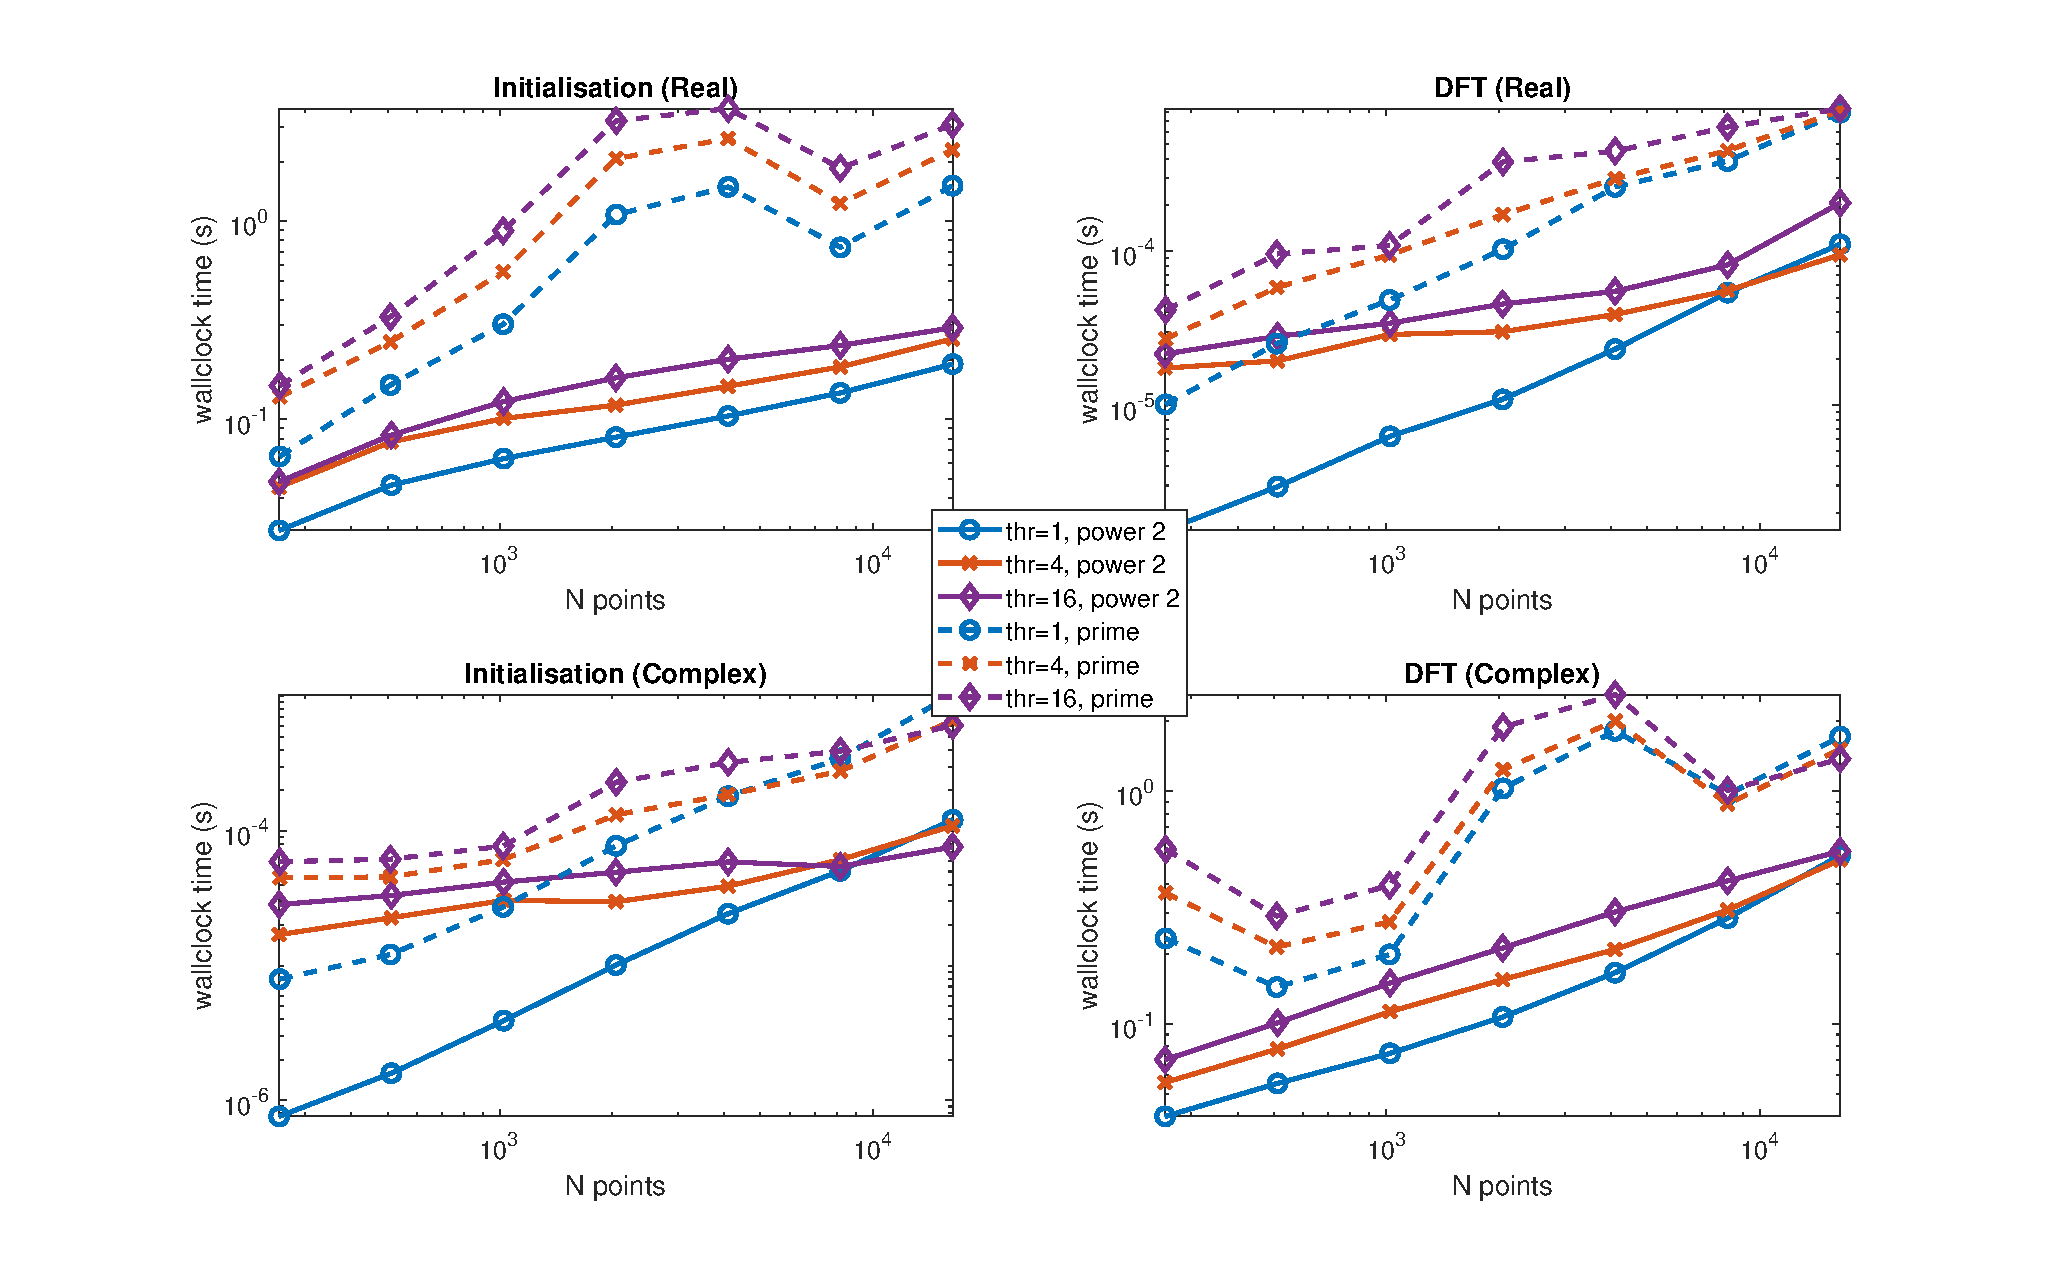
\includegraphics[width=\linewidth]{../results/fftw_1d_thr.eps}
  \caption{Initialisation and DFT execution times of FFTW library applied to 1D signal as a function of the
    number of points, $N,$ and varying the number of threads, $thr.$ }
  \label{1DFFTW}
\end{figure}


\begin{table}
\begin{center}
%\being{small}
\begin{tabular}{|r|r|r|r|r|r|r|r|r|r|}
\hline 
     \multicolumn{3}{|c|}{ } & \multicolumn{7}{c|}{$thr$} \\ \hline
    $N$  & & R/C  & 1           & 2    & 4    & 8    & 12   & 16    & 24  \\ \hline\hline
    2048  & ftime & R  &  1.09e-5 &   1.71e-5 &   3.00e-5 &   3.49e-5 &   4.05e-5 &   4.54e-5 &   6.26e-5   \\ 
      & fratio & & 1.00 &    1.57 &    2.75 &    3.20 &    3.72 &    4.17 &    5.74   \\ 
     & itime & &  8.13e-2 &    1.09e-1 &   1.18e-1 &   1.42e-1 &   1.72e-1 &   1.62e-1 &   2.14e-1    \\ 
     & iratio & &   1.00 &    1.34 &    1.45 &    1.75 &    2.12 &    1.99 &    2.63    \\ \hline 
    2053  & ftime & R &  1.03e-4 &   1.20e-4 &   1.73e-4 &   1.93e-4 &   2.50e-4 &   3.81e-4 &   7.14e-4    \\ 
      & fratio & & 1.00 &   1.17 &   1.68 &   1.87 &   2.43 &   3.70 &   6.93    \\ 
     & itime &  &   1.08e0 &   1.71e0 &   2.07e0 &   2.51e0 &   2.93e0 &   3.21e0 &   3.79e0   \\ 
    & iratio &  &     1.00 &   1.58 &   1.92 &   2.32 &   2.71 &   2.97 &   3.51     \\ \hline 
  16381  & ftime & R &  7.97e-4 &   7.98e-4 &   8.19e-4 &   8.25e-4 &   8.30e-4 &   8.47e-4 &   9.57e-4     \\ 
      & fratio & &  1.00 &   1.00 &   1.03 &   1.04 &   1.04 &   1.06 &   1.20    \\ 
     & itime & &  1.51e0 &   2.05e0 &   2.29e0 &   2.56e0 &   2.84e0 &   3.07e0 &   3.67e0     \\ 
     & iratio & &  1.00 &   1.36 &   1.52 &   1.70 &   1.88 &   2.03 &   2.43     \\ \hline 
 16384  & ftime & R & 1.11e-4 &   8.58e-5 &   9.49e-5 &   8.59e-5 &   9.79e-5 &   2.06e-4 &   5.42e-4   \\ 
      & fratio & & 1.00 &   0.77 &   0.85 &   0.77 &   0.88 &   1.86 &   4.88  \\
     & itime & & 1.90e-1 &   2.62e-1 &   2.55e-1 &   2.60e-1 &   3.07e-1 &   2.90e-1 &   3.98e-1   \\ 
 & iratio & & 1.00 &   1.38 &   1.34 &   1.37 &   1.62 &   1.53 &   2.09   \\  \hline \hline
    2048  & ftime & C  &  1.01e-5 &   1.84e-5 &   2.98e-5 &   3.39e-5 &   3.72e-5 &   4.94e-5 &   5.92e-5   \\ 
      & fratio & &  1.00 &   1.82 &   2.95 &   3.36 &   3.68 &   4.89 &   5.86  \\ 
     & itime & &   1.07e-1 &   1.16e-1 &   1.55e-1 &   1.80e-1 &   2.10e-1 &   2.12e-1 &   2.68e-1   \\ 
     & iratio & &  1.00 &   1.08 &   1.45 &   1.68 &   1.96 &   1.98 &   2.50     \\ \hline 
    2053  & ftime & C &  7.76e-5 &   1.03e-4 &   1.32e-4 &   1.81e-4 &   1.83e-4 &   2.30e-4 &   4.48e-4     \\ 
      & fratio & &  1.00 &   1.33 &   1.70 &   2.33 &   2.36 &   2.96 &   5.77   \\ 
     & itime &  &  1.03e0 &   1.06e0 &   1.24e0 &   1.47e0 &   1.74e0 &   1.89e0 &   2.21e0    \\ 
    & iratio &  &  1.00 &   1.03 &   1.20 &   1.43 &   1.69 &   1.84 &   2.15       \\ \hline
  16381  & ftime & C &   1.03e-3 &   6.76e-4 &   6.62e-4 &   6.40e-4 &   6.74e-4 &   6.07e-4 &   7.91e-4     \\ 
      & fratio & &  1.00 &   0.66 &  0.64 &   0.62 &  0.65 &   0.59 &  0.77   \\ 
     & itime & &   1.72e0 &   1.64e0 &   1.52e0 &   1.58e0 &   1.51e0 &   1.38e0 &   1.78e0    \\ 
     & iratio & &   1.00 &   0.95 &  0.88 &  0.92 &  0.88 &  0.80 &  1.03    \\ \hline
 16384  & ftime & C &  1.21e-4 &   8.86e-5 &   1.09e-4 &   8.21e-5 &   8.88e-5 &   7.61e-5 &   2.39e-4  \\ 
      & fratio & & 1.00 &   0.73 &  0.90 &  0.68 &  0.73 &  0.63 &  1.98  \\
     & itime & &  5.30e-1 &   5.01e-1 &   5.07e-1 &   5.22e-1 &   5.37e-1 &   5.53e-1 &   6.53e-1   \\ 
 & iratio & &  1.00 &   0.95 &  0.96 &  0.98 &  1.01 &   1.04 &   1.23  \\  \hline 
\end{tabular}
\caption{1D FFTW applied to real (R) and complex (C) valued one-dimensional arrays of length $N=2048,$ 2053, 16381, 16384, 1048573 and 1048576 using $thr$ threads. The wallclock DFT computation time, ftime, and wallclock DFT initialisation time, itime, both in seconds, are provided. Additionally,  the ratio, fratio, of ftime  with ftime($thr=1$) and the ratio, iratio, of itime  with itime($thr=1$) is provided. }\label{Tbl:FFTW1d}
%\end{small}
\end{center}
\end{table}

\subsection{1D MKL Library}\label{Sec:1DMKL}

The 1D MKL library benchmark runs for 1, 4 and 16 threads ($thr$) are compared
in Figure~\ref{1DMKL}. Initialisation times for $N$ a power of 2 are
nearly always lower than when $N$ is a prime number. For a single
thread, the initialisation time increased as the value of $N$
increased but the rate of increase was much larger when $N$ was
prime. For 4 or 16 threads and $N$ a power of 2, the initialisation
time stays almost constant for $N\le 2^{17}$ and then drops: in the
real case, it then starts rising again for the largest values of $N$
considered. When $N$ is a prime value and 4 or 16 threads are used,
the initialisation times remain almost constant for $N\le 2^{14}$ and
then rises with problem size for larger values of $N.$ For the smaller
values of $N,$ the initialisation times is significantly lower when
one thread is used instead of 4 or 16 (a factor of approximately 10
difference).

As expected, the DFT times are higher when $N$ is prime compared to
$N$ being a power of 2. There is little effect on the DFT time when
the number of threads is varied but $N$ is prime. However, when $N$ is
a power of 2 and greater than $2^{14}$ (real case) or $2^{17}$
(complex case), there is an advantage to using musing multiple threads
with respect to DFT wallclock time. In Table~\ref{Tbl:MKL1d}, we
provide the (wall clock) execution times of the initialisation stage
and the DFT calculations along with their ratio with respect to one
thread for $thr=1,$ 2, 4, 8, 12, 16 and 24. Results for both real and
complex input signals are given for $N=2048,$ 2053, 16381, 16384,
1048573 and 1048576. We observe that when $N$ is prime, there is
little difference between the real and complex results. The DFT time
is almost unchanged when the number of threads is increased but the
initialisation time increases significantly for the two smaller values
of $N$ in the table. Additionally, the initialisation times are
between two and three orders of magnitude larger than the DFT times
for $N=2053$ and 16381. For the largest prime value of $N$ considered,
increasing the number or threads increases the DFT time very slightly
(upto 6\% increase for 24 threads) and also results in a slight
increase in initialisation time (upto 10\%), with the initialisation
time being roughly 90\% greater than the DFT time.

For the values of $N$ that are powers of 2, the table shows that
increasing the number of threads does, in general, result in an
increase in initialisation time and for the smaller values of $N$ the
initialisation time can increase by a factor of almost 10 (real) or 6
(complex): given that there is little difference in DFT time for
differing numbers of threads, we do not advocate using multiple
threads for these smaller values of $N.$ For $N=1048576$ increasing
the number of threads from a single thread results in at most an
increase of 79\% (real) or 32\% (complex) in initialisation time. For
the real case, 16 threads reduces the DFT time by a factor of ~4 and,
for the complex case, the DFT time is reduced by a factor of
~2.4. Given that the initialisation and DFT times are at most a factor
of 10 different, only a small number of DFT computations are required
to overcome the increase in initialisation time.


\begin{figure}[htb]
    \centering
    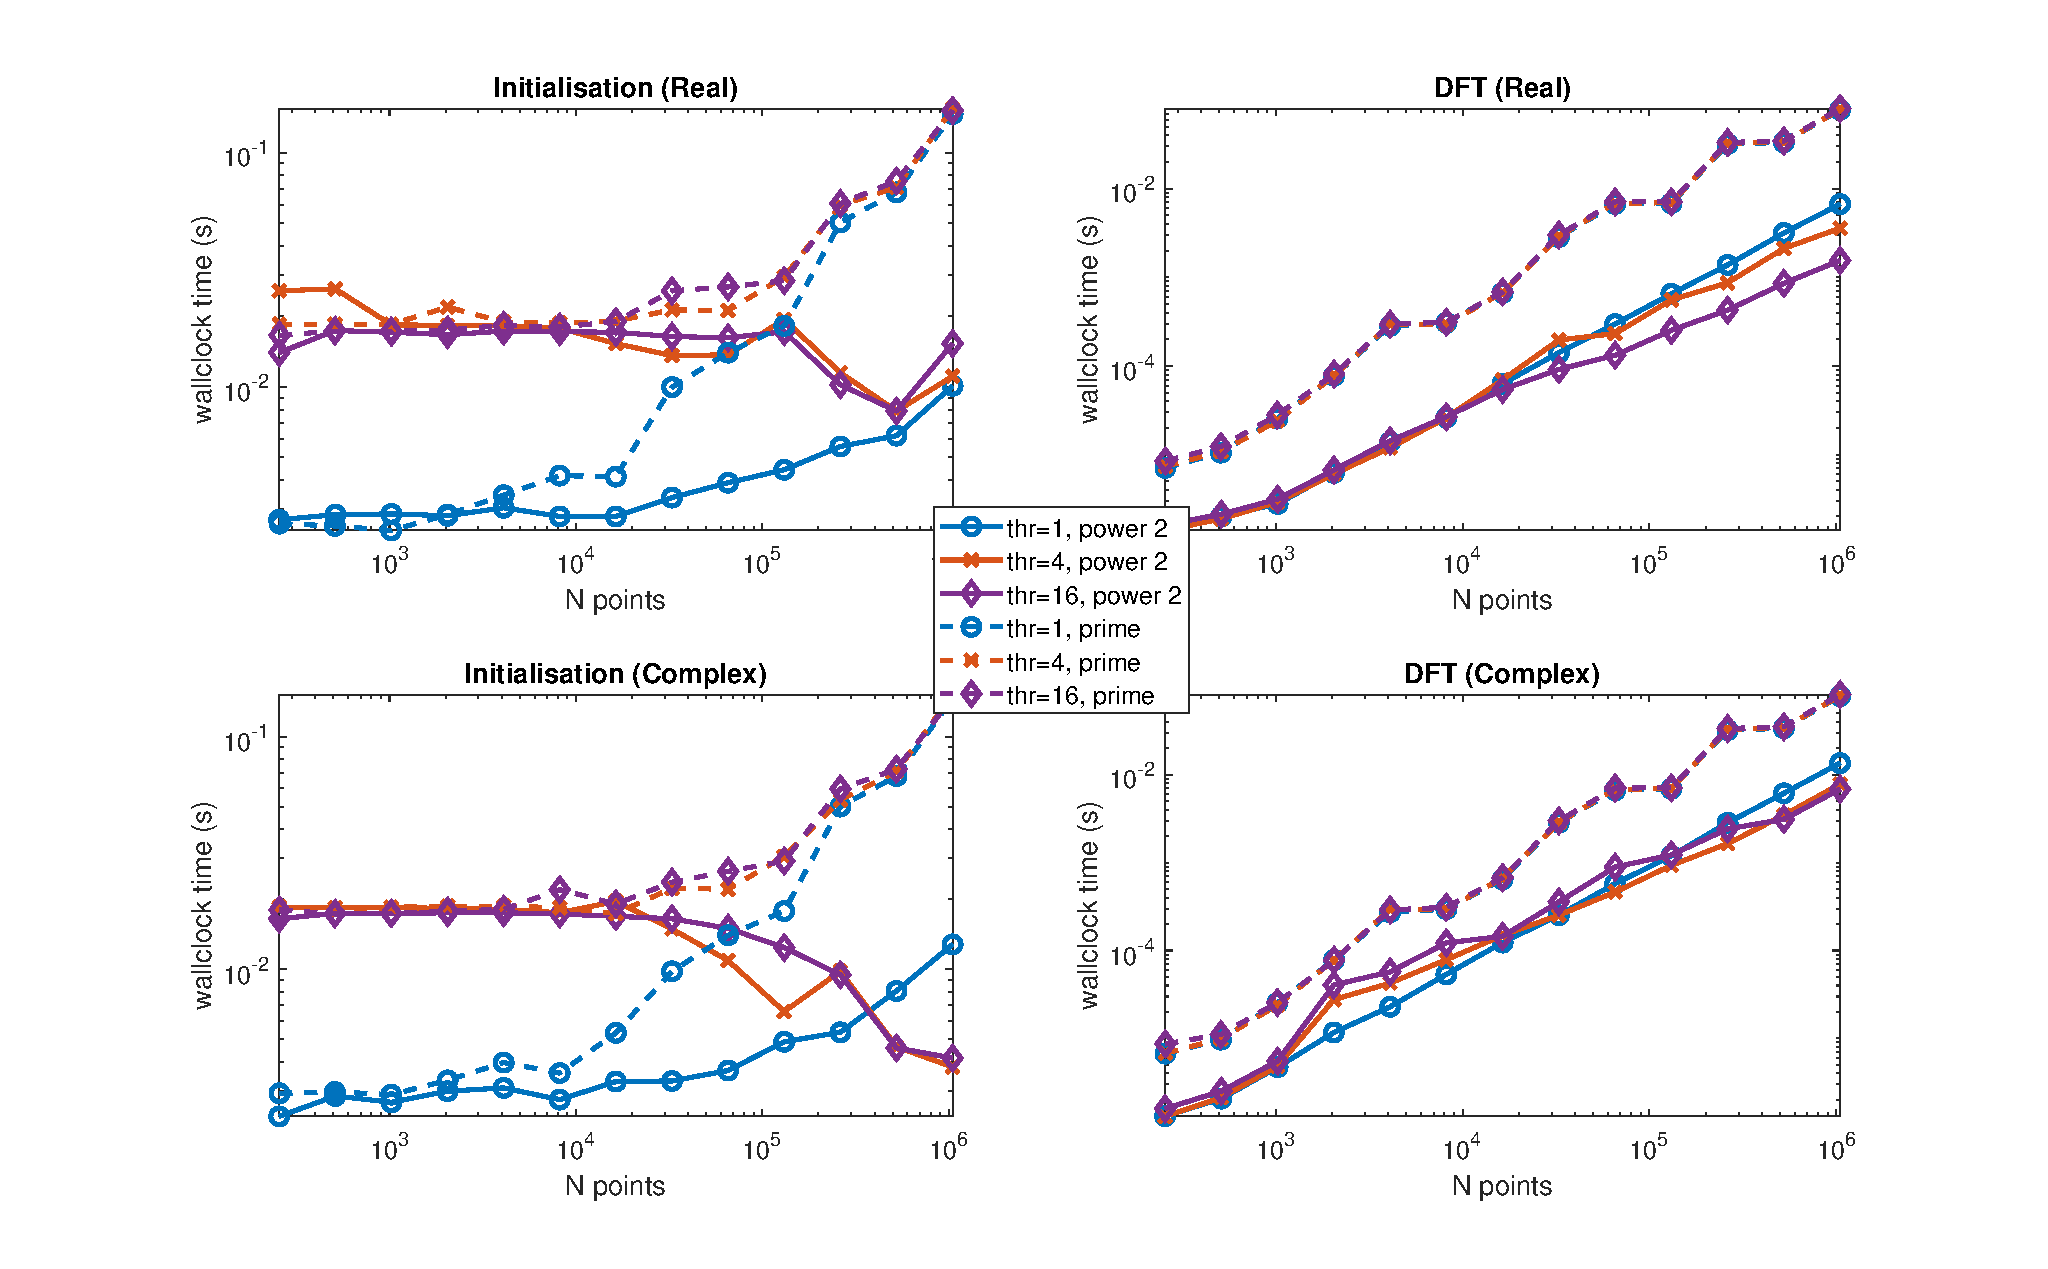
\includegraphics[width=\linewidth]{../results/mkl_1d_thr.eps}
  \caption{Initialisation and DFT execution times of MKL library applied to 1D signal as a function of the
    number of points, $N,$ and varying the number of threads, $thr.$ }
  \label{1DMKL}
\end{figure}


\begin{table}
\begin{center}
%\being{small}
\begin{tabular}{|r|r|r|r|r|r|r|r|r|r|}
\hline 
     \multicolumn{3}{|c|}{ } & \multicolumn{7}{c|}{$thr$} \\ \hline
    $N$  & & R/C  & 1           & 2    & 4    & 8    & 12   & 16    & 24  \\ \hline\hline
    2048  & ftime & R  &  6.21e-6 &   8.79e-6 &   6.05e-6 &   6.38e-6 &   7.32e-6 &   6.69e-6 &   7.08e-6  \\ 
      & fratio & & 1.00 &   1.42 &   0.97 &   1.03 &   1.13 &   1.03 &   1.14   \\ 
     & itime & &    2.82e-3 &   1.27e-2 &   1.83e-2 &   1.72e-2 &   1.75e-2 &   1.67e-2 &   1.66e-2   \\ 
     & iratio & &   1.00 &   4.50 &   6.49 &   6.10 &   6.21 &   5.92 &   5.89    \\ \hline 
    2053  & ftime & R &  7.74e-5 & 7.99e-5 &   7.77e-5 &   1.06e-4 &   8.25e-5 &   8.11e-5 &   8.33e-5    \\ 
      & fratio & &  1.00 &   1.03 &   1.00 &   1.37 &   1.07 &   1.05 &   1.08   \\ 
     & itime &  &   2.85e-3 &   1.26e-2 &   2.19e-2 &   2.59e-2 &   1.40e-2 &   1.75e-2 &   1.69e-2    \\ 
    & iratio &  &     1.00 &   4.42 &   7.68 &   9.09 &   4.91 &   6.14 &   5.93     \\ \hline 
  16381  & ftime & R &  6.68e-4 &   6.47e-4 &   6.73e-4 &   6.81e-4 &   6.68e-4 &   6.84e-4 &   7.32e-4      \\ 
      & fratio & &  1.00 &   0.97 &   1.01 &   1.02 &   1.00 &   1.02 &   1.10    \\ 
     & itime & &   4.14e-3 &   1.31e-2 &   1.91e-2 &   2.75e-2 &   1.92e-2 &   1.90e-2 &   2.29e-2    \\ 
     & iratio & &  1.00 &   3.16 &   4.61 &   6.64 &   4.64 &   4.59 &   5.53     \\ \hline 
 16384  & ftime & R &  6.30e-5 &   6.74e-5 &   6.98e-5 &   5.49e-5 &   6.03e-5 &   5.41e-5 &   6.23e-5   \\ 
      & fratio & &   1.00 &   1.07 &   1.11 &   0.87 &  0.96 &   0.86 &   0.99 \\
     & itime & &  2.80e-3 &   2.68e-3 &   1.53e-2 &   2.59e-2 &   1.70e-2 &   1.71e-2 &   1.60e-2   \\ 
 & iratio & &  1.00 &   0.96 &   5.46 &   9.25 &   6.07 &   6.11 &   5.71   \\  \hline 
  1048573  & ftime & R &    7.78e-2 &   7.74e-2 &   7.84e-2 &   7.97e-2 &   8.04e-2 &   8.03e-2 &   8.02e-2    \\ 
      & fratio & &  1.00 &   0.99 &   1.01 &   1.02 &   1.03 &   1.03 &   1.03    \\ 
     & itime & &   1.46e-1 &   1.48e-1 &   1.54e-1 &   1.57e-1 &   1.49e-1 &   1.51e-1 &   1.58e-1    \\ 
     & iratio & &   1.00 &   1.01 &   1.05 &   1.08 &   1.02 &   1.03 &   1.08    \\ \hline 
 1048576  & ftime & R &  6.71e-3 &   6.21e-3 &   3.59e-3 &   2.17e-3 &   2.31e-3 &   1.55e-3 &   1.78e-3   \\ 
      & fratio & & 1.00 &   0.93 &   0.54 &   0.32 &   0.34 &   0.23 &   0.27  \\
     & itime & & 1.01e-2 &   1.79e-2 &   1.11e-2 &   1.20e-2 &   6.88e-3 &   1.53e-2 &   1.81e-2    \\ 
 & iratio & &  1.00 &   1.77 &   1.10 &   1.19 &   0.68 &   1.51 &   1.79   \\  \hline \hline
    2048  & ftime & C  &  1.17e-5 &   1.99e-5 &   2.76e-5 &   3.92e-5 &   3.78e-5 &   4.06e-5 &   3.64e-5   \\ 
      & fratio & &  1.00 &   1.70 &   2.36 &   3.35 &   3.23 &   3.47 &   3.11   \\ 
     & itime & &  2.99e-3 &   1.26e-2 &   1.83e-2 &   1.86e-2 &   1.76e-2 &   1.75e-2 &   1.63e-2   \\ 
     & iratio & &  1.00 &   4.21 &   6.12 &   6.22 &   5.89 &   5.85 &   5.45    \\ \hline 
    2053  & ftime & C &  7.81e-5 &   7.73e-5 &   7.77e-5 &   7.87e-5 &   7.92e-5 &   7.76e-5 &   8.06e-5     \\ 
      & fratio & & 1.00 &   0.99 &   0.99 &   1.01 &   1.01 &   0.99 &   1.03    \\ 
     & itime &  & 3.33e-3 &   1.32e-2 &   1.87e-2 &   2.25e-2 &   2.21e-2 &   1.78e-2 &   1.74e-2    \\ 
    & iratio &  &    1.00 &   3.96 &   5.62 &   6.76 &   6.64 &   5.35 &   5.23     \\ \hline
  16381  & ftime & C &    6.42e-4 &   6.65e-4 &   6.66e-4 &   6.77e-4 &   6.67e-4 &   6.74e-4 &   7.02e-4     \\ 
      & fratio & & 1.00 &   1.04 &   1.04 &   1.05 &   1.04 &   1.05 &   1.09    \\ 
     & itime & &    5.33e-3 &   1.29e-2 &   1.74e-2 &   2.69e-2 &   2.32e-2 &   1.91e-2 &   1.91e-2    \\ 
     & iratio & &    1.00 &   2.42 &   3.26 &   5.05 &   4.35 &   3.58 &   3.58  \\ \hline
 16384  & ftime & C &  1.23e-4 &   1.15e-4 &   1.49e-4 &   1.39e-4 &   1.38e-4 &   1.45e-4 &   1.17e-4   \\ 
      & fratio & & 1.00 &   0.93 &   1.21 &   1.13 &   1.12 &   1.18 &   0.95  \\
     & itime & &  3.29e-3 &   1.07e-2 &   1.96e-2 &   1.70e-2 &   1.68e-2 &   1.69e-2 &   1.59e-2   \\ 
 & iratio & & 1.00 &   3.25 &   5.96 &   5.17 &   5.11 &   5.14 &   4.83   \\  \hline 
  1048573  & ftime & C &  7.80e-2 &   7.78e-2 &   7.88e-2 &   8.01e-2 &   8.06e-2 &   8.13e-2 &   8.25e-2      \\ 
      & fratio & &  1.00 &   1.00 &   1.01 &   1.03 &   1.03 &   1.04 &   1.06    \\ 
     & itime & &   1.46e-1 &   1.49e-1 &   1.52e-1 &   1.60e-1 &   1.50e-1 &   1.47e-1 &   1.59e-1   \\ 
     & iratio & &    1.00 &   1.02 &   1.04 &   1.10 &   1.03 &   1.01 &   1.09    \\ \hline 
 1048576  & ftime & C &  1.35e-2 &   1.37e-2 &   7.80e-3 &   5.64e-3 &   5.54e-3 &   6.83e-3 &   7.87e-3   \\ 
      & fratio & &  1.00 &   1.01 &   0.58 &   0.42 &   0.41 &   0.51 &   0.58  \\
     & itime & &  1.28e-2 &   3.83e-3 &   3.80e-3 &   1.52e-2 &   1.49e-2 &   4.15e-3 &   1.69e-2   \\ 
 & iratio & &  1.00 &   0.30 &   0.30 &   1.19 &   1.16 &   0.32 &   1.32 
  \\  \hline 
\end{tabular}
\caption{1D MKL applied to real (R) and complex (C) valued one-dimensional arrays of length $N=2048,$ 2053, 16381, 16384, 1048573 and 1048576  using $thr$ threads. The wallclock DFT computation time, ftime, and wallclock DFT initialisation time, itime, both in seconds, are provided. Additionally,  the ratio, fratio, of ftime  with ftime($thr=1$) and the ratio, iratio, of itime  with itime($thr=1$) is provided. }\label{Tbl:MKL1d}
%\end{small}
\end{center}
\end{table}



\subsection{Comparison of libraries for 1D benchmarks}\label{Sec:1DComp}

In Figure~\ref{1DFFTWMKL2}, we compare the 1D FFTW and MKL libraries
with multithreading for values of $N$ that are prime numbers. Our
first observation is that, in our computing environment, the MKL
library can perform DFT computations for larger values of $N.$ For the
values of $N$ where we can compare the libraries, MKL has
significantly lower initialisation times. For DFT times, in the real
case, MKL is always faster than FFTW but in the complex case, the MKL
library is best for the very small values of $N$ but as we approach
$N=16384,$ the times appear to be similar. Given the substantial
difference in initialisation time and the larger values of $N$
available for use by the user, we recommend that the MKL library is
used.



\begin{figure}[htb]
    \centering
    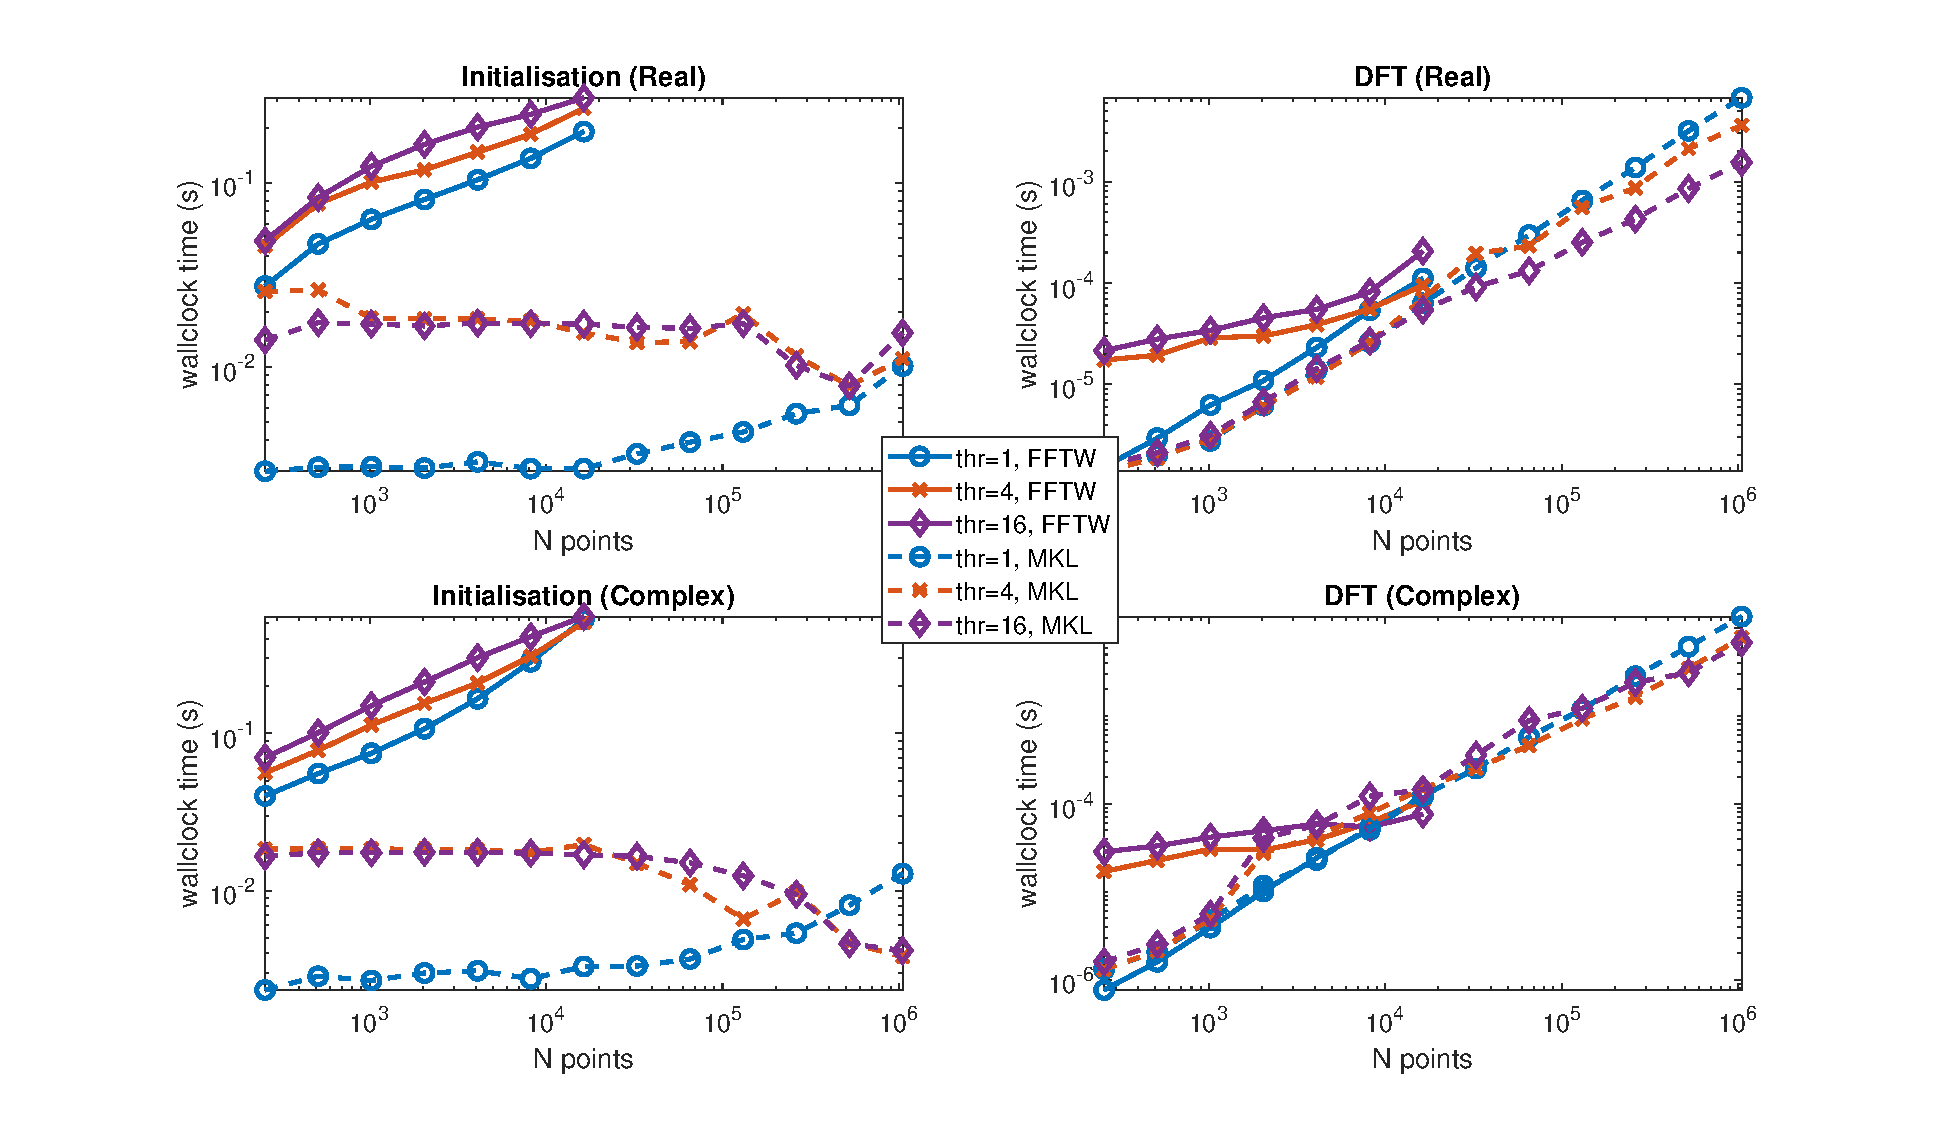
\includegraphics[width=\linewidth]{../results/fftw_mkl_2_1d_thr.eps}
  \caption{Initialisation and DFT execution times of FFTW and MKL libraries applied to 1D signal as a function of the
    number of points, $N,$ and varying the number of threads, $thr.$ $N$ is a power of 2.}
  \label{1DFFTWMKL2}
\end{figure}



The FFTW and MKL libraries are compared in Figure~\ref{1DFFTWMKLPrime}
for prime values of $N.$ As with the case when $N$ is a power of 2,
the initialisation times are significantly lower for the MKL
library. The difference in DFT times is not as pronounced as in the
former case but MKL is still generally faster than FFTW (although, if
the library could accommodate larger values of $N,$ FFTW looks like it
would be faster for these values). Therefore, when $N$ is a prime
number, we recommend using the MKL library over the FFTW library.

\begin{figure}[htb]
    \centering
    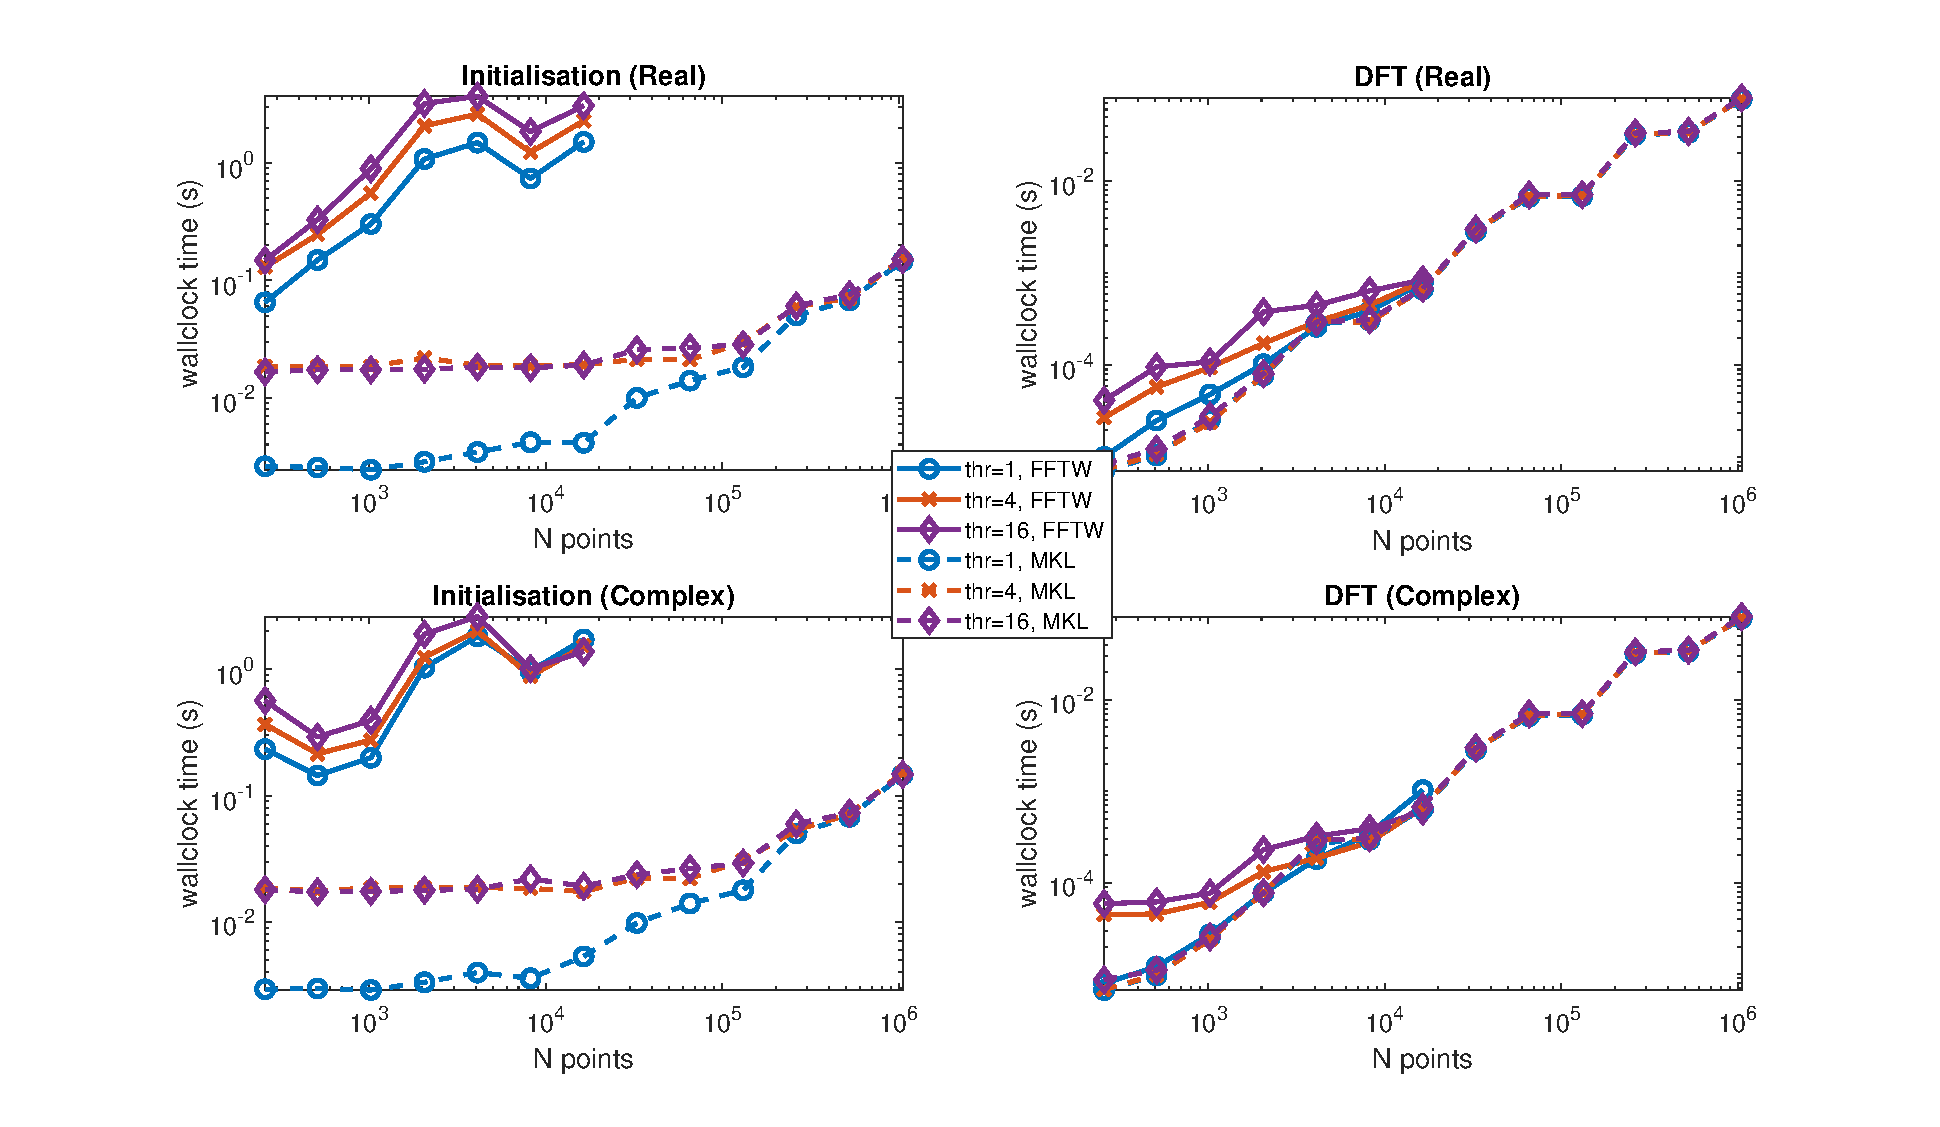
\includegraphics[width=\linewidth]{../results/fftw_mkl_prime_1d_thr.eps}
  \caption{Initialisation and DFT execution times of FFTW and MKL libraries applied to 1D signal as a function of the
    number of points, $N,$ and varying the number of threads, $thr.$ $N$ is a prime number.}
  \label{1DFFTWMKLPrime}
\end{figure}


\section{Effect of domain size and multithreading for 2D benchmarks}\label{Sec:2DMulti}
The benchmark results for libraries that perfrom the fast Fourier
transform over a 2D domain are discussed in this section. As with the
1D results in Section~\ref{Sec:1DMulti}, the P3DFFT library cannot be
used on these problems so we compare the OpenMP versions of the FFTW
and MKL libraries.

Similarly to the benchmarks in Section~\ref{Sec:1DMulti}, we set
$n_3=4,$ $n_q=4$ and $n_1=n_2=N,$ were $N$ is defined as follows.  For one
set of tests, we let $N=2^k$ for $k=5,\ldots,12.$ For the other set of
tests, $N$ is defined to be the closest prime number to $2^k,$
$k=5,\ldots,12:$ if two primes are equidistant, we choose the larger
one.

\subsection{2D FFTW Library}\label{Sec:2DFFTW}

In Figure~\ref{2DFFTW}, we compare our single node benchmark
experiments for the multithreaded FFTW library with 1, 4 and 16 OpenMP
threads. There is a difference in behaviour between the real and
complex benchmarks. For $N$ smaller than 200, the initialisation times
for the real case are smaller when $N$ is prime compared to when $N$
is a power of 2; for the complex case, the initialisation times for
$N$ prime are, in general, greater than $N$ a power of 2. For larger
values of $N,$ the initialisation times for prime values of $N$ are
larger than $N$ a power of 2 in both the real and complex cases but
the complex initialisation times appear to be higher than in the real
case. Increasing the number of threads also increases the
initialisation times but, as the problem size increases, the
difference between 4 and 16 threads generally diminishes. For further
clarity of the benchmark results, we provide the (wall clock)
execution times of the initialisation stage and the DFT calculations
along with their ratio with respect to one thread for $thr=1,$ 2, 4,
8, 12, 16 and 24 in Table~\ref{Tbl:FFTW2d}. Results for both real and
complex input signals are given for $N=31,$ 32, 256, 257, 2048 and
2053. These confirm that the initialisation times are lower for the
real case compared to the complex case. Additionally, increasing the
number of threads has less of an effect when $N$ is prime compared to
when $N$ is a power of 2. However,

Comparing the DFT times in Figure~\ref{2DFFTW}, for the larger values
of $N,$ increasing the number of threads is always improving the
wallclock time. When $N$ is a power of 2, a single thread is
prefereable for $N\le 128.$ The DFT times are larger when $N$ is a
prime number instead of being a power of 2. Using
Table~\ref{Tbl:FFTW2d}, we see observe that increasing the number of
threads results in lower ratios when $N$ is a prime compared to when
$N$ is a power of 2. Given that the initialisation times are at least
one order of magnitude larger than the DFT times, when a small number
of DFT calculations are being performed with a single initialisation,
it is normally best to use a single thread when $N$ is small (less
than 300) but for a large value of $N$ we recommend using 16 or 24
threads (the latter if performing a large number of DFT calculations).




\begin{figure}[htb]
    \centering
    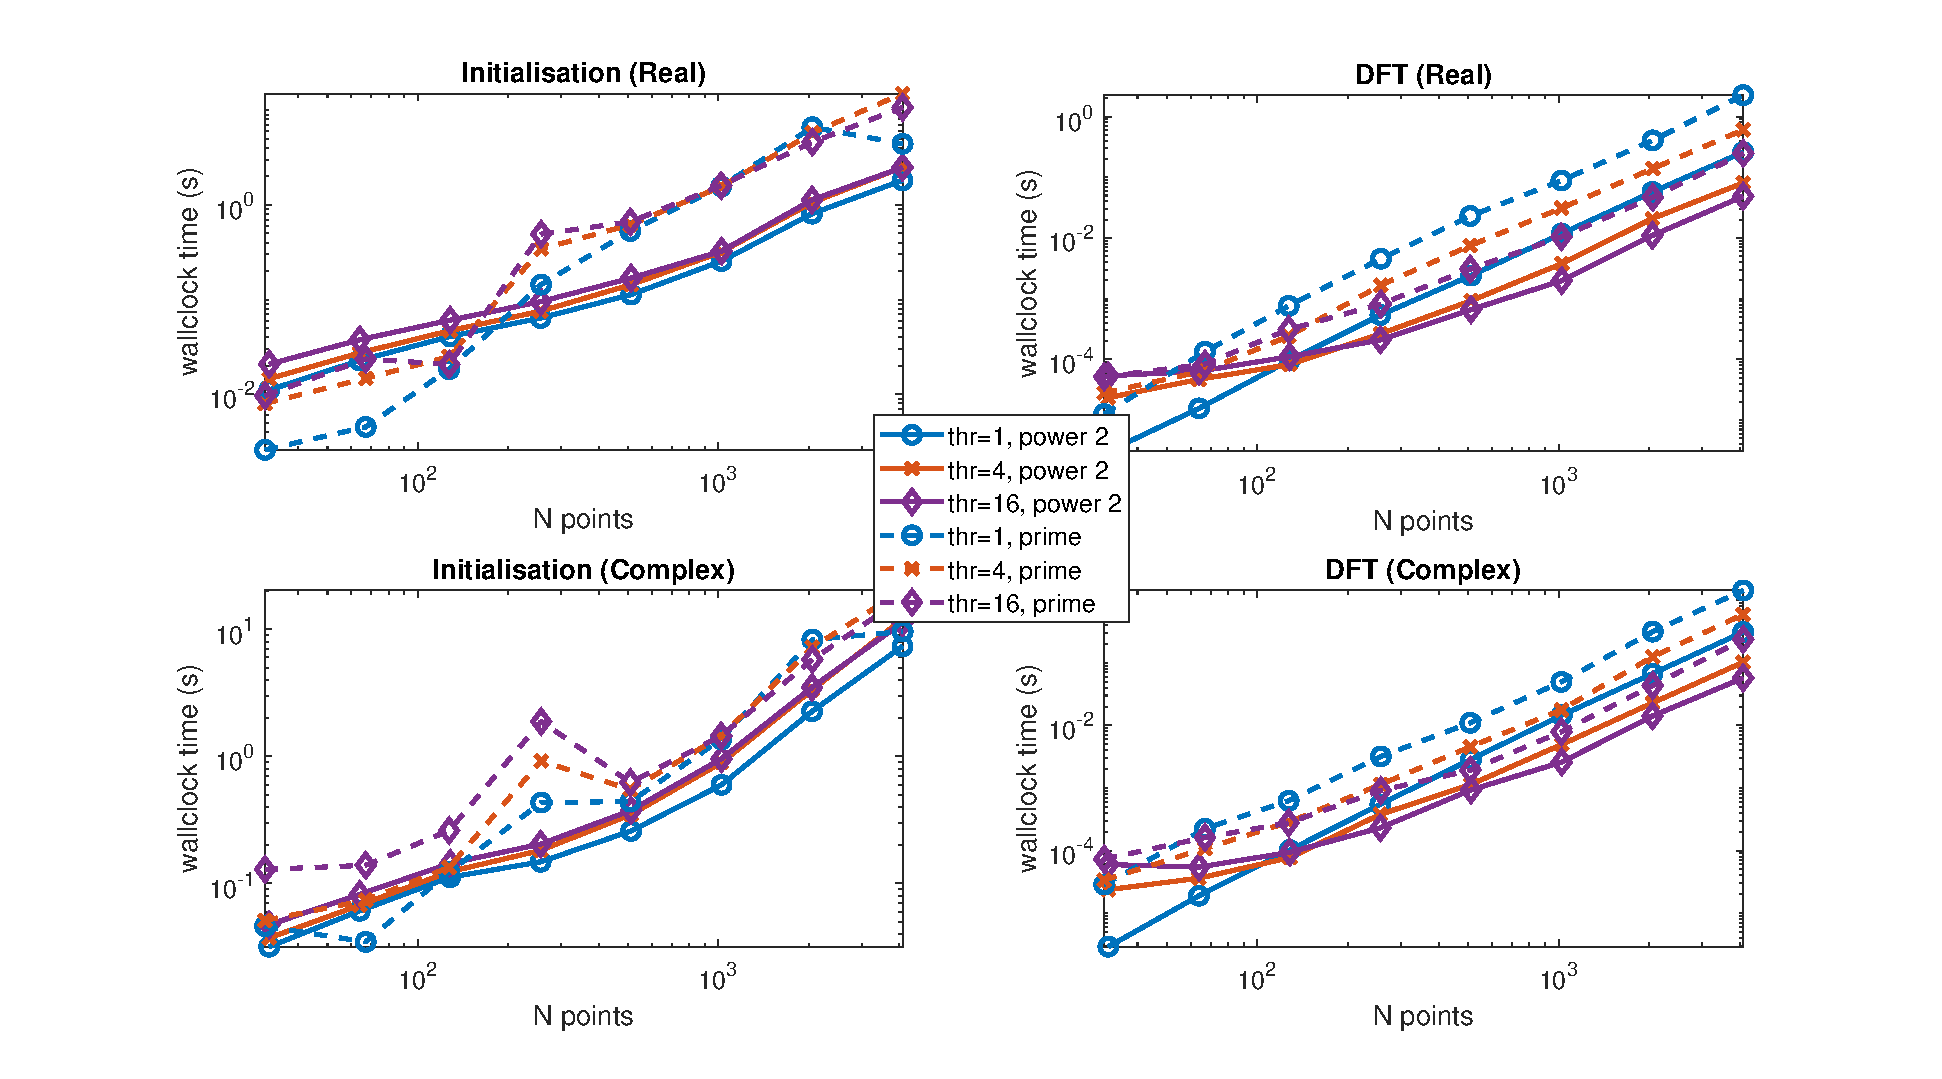
\includegraphics[width=\linewidth]{../results/fftw_2d_thr.eps}
  \caption{Initialisation and DFT execution times of FFTW library applied to 2D signal as a function of the
    number of points, $N,$ and varying the number of threads, $thr.$ }
  \label{2DFFTW}
\end{figure}

\begin{table}
\begin{center}
%\being{small}
\begin{tabular}{|r|r|r|r|r|r|r|r|r|r|}
\hline 
     \multicolumn{3}{|c|}{ } & \multicolumn{7}{c|}{$thr$} \\ \hline
    $N$  & & R/C  & 1           & 2    & 4    & 8    & 12   & 16    & 24  \\ \hline\hline
    31  & ftime & R  &  1.26e-5 &   3.50e-5 &   2.81e-5 &   3.39e-5 &   6.63e-5 &   5.16e-5 &   7.92e-5   \\ 
      & fratio & &      1.00 &   2.78 &   2.23 &   2.69 &   5.26 &   4.10 &   6.29     \\ 
     & itime & &        2.59e-3 &   8.92e-3 &   8.00e-3 &   9.38e-3 &   1.55e-2 &   9.68e-3 &   1.39e-2     \\ 
     & iratio & &       1.00 &   3.44 &   3.09 &   3.62 &   5.98 &   3.74 &   5.37      \\ \hline 
    32  & ftime & R  &  3.05e-6 &   2.28e-5 &   2.34e-5 &   3.47e-5 &   5.42e-5 &   5.36e-5 &   8.02e-5   \\ 
      & fratio & &      1.00 &   7.48 &   7.67 &   11.4 &   17.8 &   17.6 &   26.3     \\ 
     & itime & &        1.11e-2 &   1.51e-2 &   1.46e-2 &   1.80e-2 &   4.30e-2 &   2.08e-2 &   2.55e-2     \\ 
     & iratio & &       1.00 &   1.36 &   1.32 &   1.62 &   3.87 &   1.87 &   2.30      \\ \hline 
   256  & ftime & R  &  5.38e-4 &   3.57e-4 &   2.63e-4 &   2.23e-4 &   2.08e-4 &   2.09e-4 &   2.36e-4   \\ 
      & fratio & &      1.00 &   0.66 &   0.49 &   0.41 &   0.39 &   0.39 &   0.44     \\ 
     & itime & &        6.39e-2 &   7.77e-2 &   7.55e-2 &   8.82e-2 &   1.09e-1 &   9.52e-2 &   1.38e-1     \\ 
     & iratio & &       1.00 &   1.22 &   1.18 &   1.38 &   1.71 &   1.49 &   2.16      \\ \hline 
   257  & ftime & R  &  4.55e-3 &   2.56e-3 &   1.67e-3 &   1.26e-3 &   7.97e-4 &   8.17e-4 &   8.08e-4   \\ 
      & fratio & &      1.00 &   0.56 &   0.37 &   0.28 &   0.18 &   0.18 &   0.18     \\ 
     & itime & &        1.44e-1 &   2.47e-1 &   3.43e-1 &   3.81e-1 &   4.80e-1 &   4.92e-1 &   6.23e-1     \\ 
     & iratio & &       1.00 &   1.72 &   2.38 &   2.65 &   3.33 &   3.42 &   4.33      \\ \hline 
  2048  & ftime & R  &  5.71e-2 &   3.30e-2 &   2.09e-2 &   1.04e-2 &   1.22e-2 &   1.10e-2 &   1.04e-2   \\ 
      & fratio & &      1.00 &   0.58 &   0.37 &   0.18 &   0.21 &   0.19 &   0.18     \\ 
     & itime & &        8.09e-1 &   1.31e0 &   1.06e0 &   1.02e0 &   1.42e0 &   1.13e0 &   1.28e0     \\ 
     & iratio & &       1.00 &   1.62 &   1.31 &   1.26 &   1.76 &   1.40 &   1.58      \\ \hline 
  2053  & ftime & R  &  4.05e-1 &   2.44e-1 &   1.39e-1 &   8.00e-2 &   5.74e-2 &   4.66e-2 &   3.28e-2   \\ 
      & fratio & &      1.00 &   0.60 &   0.34 &   0.20 &   0.14 &   0.12 &   0.08    \\ 
     & itime & &        6.62e0 &   7.76e0 &   5.77e0 &   4.95e0 &   4.03e0 &   4.61e0 &   4.96e0     \\ 
     & iratio & &       1.00 &   1.17 &   0.87 &   0.75 &   0.61 &   0.70 &   0.75      \\ \hline \hline
    31  & ftime & C  &  2.86e-5 &   2.89e-5 &   3.37e-5 &   4.04e-5 &   6.06e-5 &   7.31e-5 &   1.10e-4   \\ 
      & fratio & &      1.00 &   1.01 &   1.18 &   1.41 &   2.12 &   2.56 &   3.85     \\ 
     & itime & &        4.60e-2 &   5.31e-2 &   5.12e-2 &   8.48e-2 &   9.37e-2 &   1.29e-1 &   1.61e-1     \\ 
     & iratio & &       1.00 &   1.15 &   1.11 &   1.84 &   2.04 &   2.80 &   3.50      \\ \hline 
    32  & ftime & C  &  2.91e-6 &   1.33e-5 &   2.37e-5 &   3.49e-5 &   6.83e-5 &   5.98e-5 &   8.59e-5   \\ 
      & fratio & &      1.00 &   4.57 &   8.14 &   12.0 &   23.5 &   20.6 &   29.5     \\ 
     & itime & &        3.18e-2 &   3.82e-2 &   3.73e-2 &   3.80e-2 &   5.56e-2 &   4.73e-2 &   5.17e-2     \\ 
     & iratio & &       1.00 &   1.20 &   1.17 &   1.20 &   1.75 &   1.49 &   1.63      \\ \hline 
   256  & ftime & C  &  5.46e-4 &   3.52e-4 &   3.79e-4 &   3.39e-4 &   2.56e-4 &   2.31e-4 &   3.10e-4   \\ 
      & fratio & &      1.00 &   0.64 &   0.69 &   0.62 &   0.47 &   0.42 &   0.57     \\ 
     & itime & &        1.48e-1 &   1.85e-1 &   1.82e-1 &   1.85e-1 &   2.08e-1 &   2.04e-1 &   2.47e-1     \\ 
     & iratio & &       1.00 &   1.25 &   1.23 &   1.25 &   1.41 &   1.38 &   1.67      \\ \hline 
   257  & ftime & C  &  3.19e-3 &   2.06e-3 &   1.14e-3 &   1.12e-3 &   9.98e-4 &   9.11e-4 &   9.06e-4   \\ 
      & fratio & &      1.00 &   0.65 &   0.36 &   0.35 &   0.31 &   0.29 &   0.28     \\ 
     & itime & &        4.33e-1 &   6.85e-1 &   9.20e-1 &   1.33e0 &   1.53e0 &   1.88e0 &   2.36e0     \\ 
     & iratio & &       1.00 &   1.58 &   2.12 &   3.07 &   3.53 &   4.34 &   5.45      \\ \hline 
  2048  & ftime & C  &  6.70e-2 &   4.04e-2 &   2.28e-2 &   1.55e-2 &   1.32e-2 &   1.41e-2 &   1.27e-2   \\ 
      & fratio & &      1.00 &   0.60 &   0.34 &   0.23 &   0.20 &   0.21 &   0.19     \\ 
     & itime & &        2.26e0 &   3.85e0 &   3.33e0 &   3.34e0 &   3.55e0 &   3.49e0 &   3.66e0     \\ 
     & iratio & &       1.00 &   1.70 &   1.47 &   1.48 &   1.57 &   1.54 &   1.62      \\ \hline 
  2053  & ftime & C  &  3.14e-1 &   1.95e-1 &   1.25e-1 &   5.44e-2 &   4.64e-2 &   4.33e-2 &   3.41e-2   \\ 
      & fratio & &      1.00 &   0.62 &   0.40 &   0.17 &   0.15 &   0.14 &   0.11     \\ 
     & itime & &        8.30e0 &   1.11e+1 &   7.21e0 &   6.07e0 &   5.49e0 &   5.78e0 &   6.33e0     \\ 
     & iratio & &       1.00 &   1.34 &   0.87 &   0.73 &   0.66 &   0.70 &   0.76      \\ \hline \hline
\end{tabular}
\caption{2D FFTW applied to real (R) and complex (C) valued two-dimensional square arrays with length $N=31,$ 32, 256, 257, 2048 and 2053 along each side and using $thr$ threads. The wallclock DFT computation time, ftime, and wallclock DFT initialisation time, itime, both in seconds, are provided. Additionally,  the ratio, fratio, of ftime  with ftime($thr=1$) and the ratio, iratio, of itime  with itime($thr=1$) is provided. }\label{Tbl:FFTW2d}
%\end{small}
\end{center}
\end{table}

\subsection{2D MKL Library}\label{Sec:2DMKL}

In Figure~\ref{2DMKL} we do the same comparisions as in
Figure~\ref{2DFFTW} but for the MKL library. For a single thread, when
$N$ is lower than 600, the initialisation times remain roughly
constant as $N$ increases and, once $N$ is greater than 600, the
initialisation time increases but at a faster rate for real signal
inputs. When mulitple threads are used, the initialisation time is
initially high but starts to decrease as $N$ increases. For 16
threads, this decrease starts sooner when the input signal is complex
and, once $N$ is greater than 1000, the multiple threads leads to
smaller initialisation times than when a signal thread is used; in the
real case, the multithreads have improved initialisation times for
$N>2000.$ In general, there is little difference between $N$ being
prime and a power of 2 for one or 16 threads with real input signals
although, for the lareger values of $N$, the initialisation time is
better when $N$ is a power of 2. For complex input signals, switching
between $N$ being a power of two and $N$ being prime has little effect
on the initialisation time when one or four threads is used. 


\begin{figure}[htb]
    \centering
    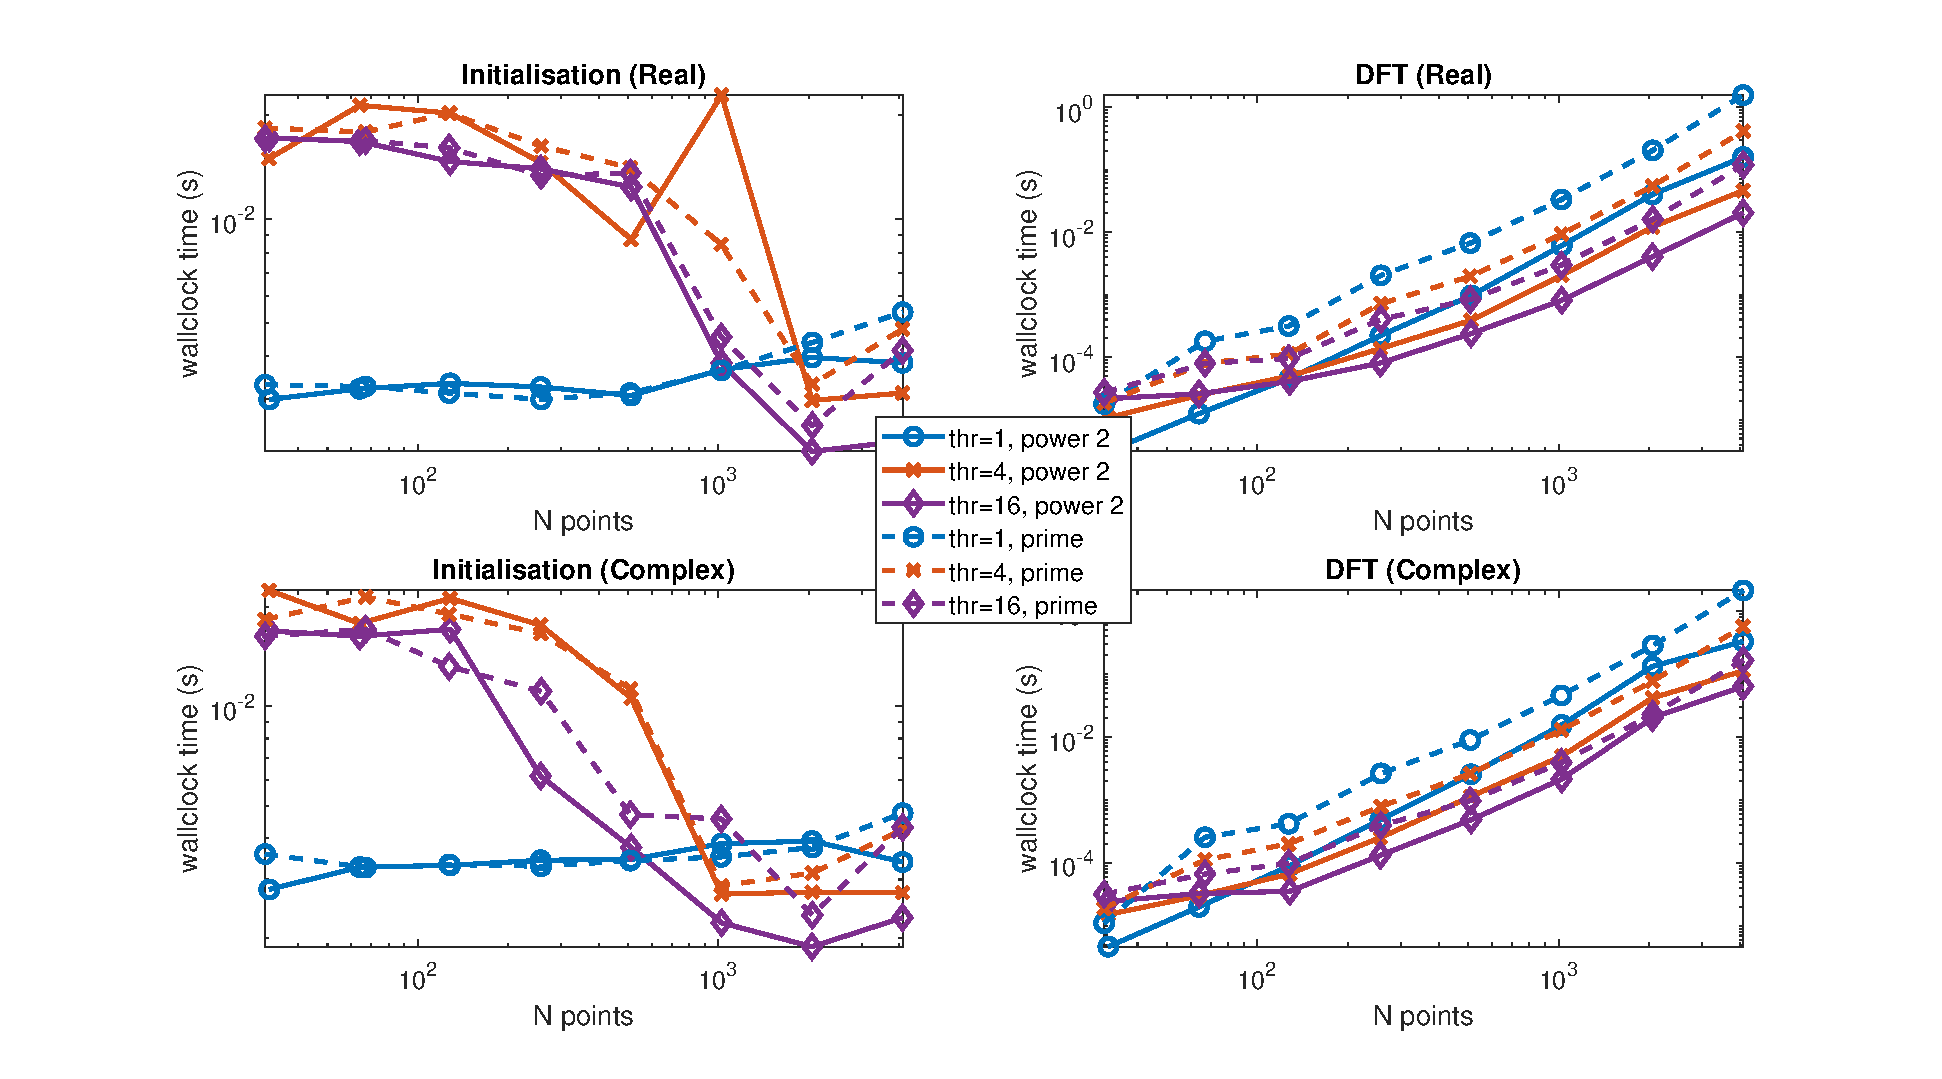
\includegraphics[width=\linewidth]{../results/mkl_2d_thr.eps}
  \caption{Initialisation and DFT execution times of MKL library applied to 2D signal as a function of the
    number of points, $N,$ and varying the number of threads, $thr.$ }
  \label{2DMKL}
\end{figure}


\subsection{Comparison of libraries for 2D benchmarks}\label{Sec:2DComp}




\begin{figure}[htb]
    \centering
    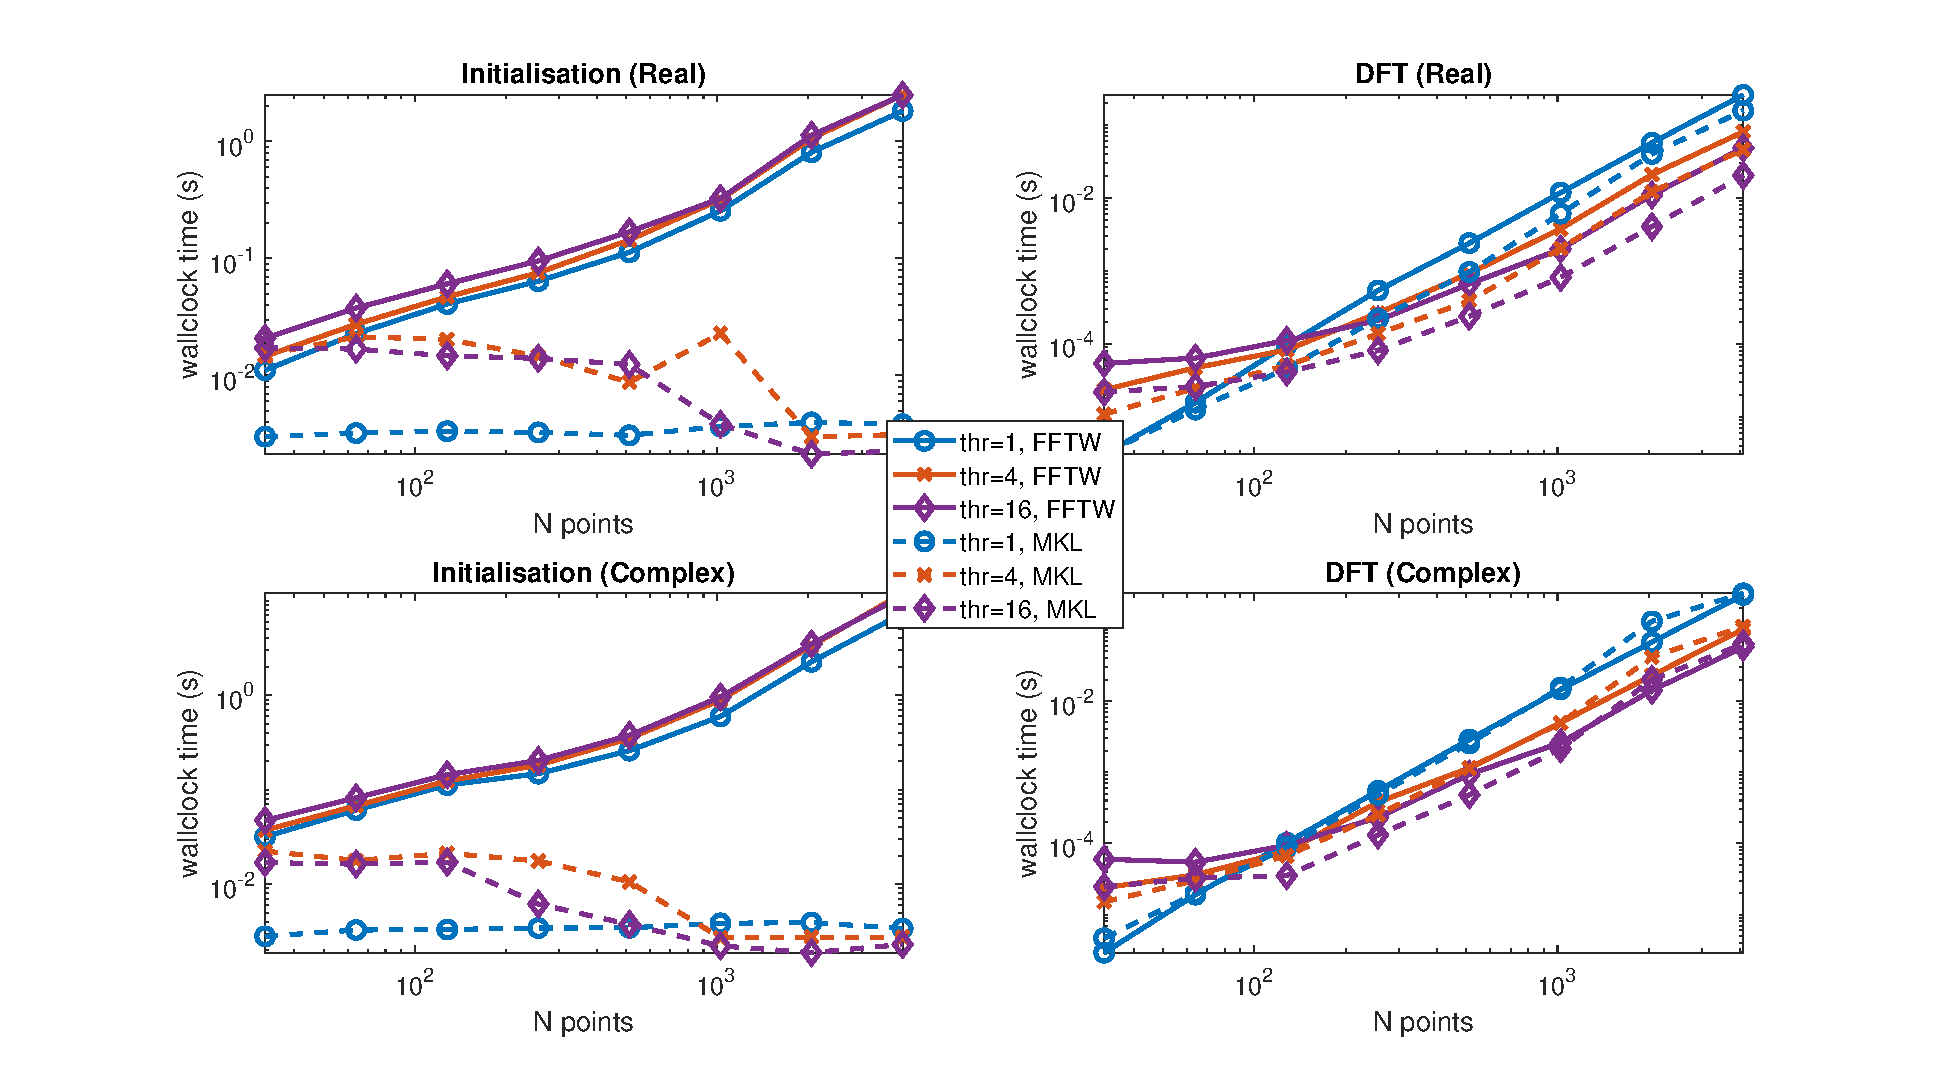
\includegraphics[width=\linewidth]{../results/fftw_mkl_2_2d_thr.eps}
  \caption{Initialisation and DFT execution times of FFTW and MKL libraries applied to 2D signal as a function of the
    number of points, $N,$ and varying the number of threads, $thr.$ $N$ is a power of 2.}
  \label{2DFFTWMKL2}
\end{figure}


\begin{figure}[htb]
    \centering
    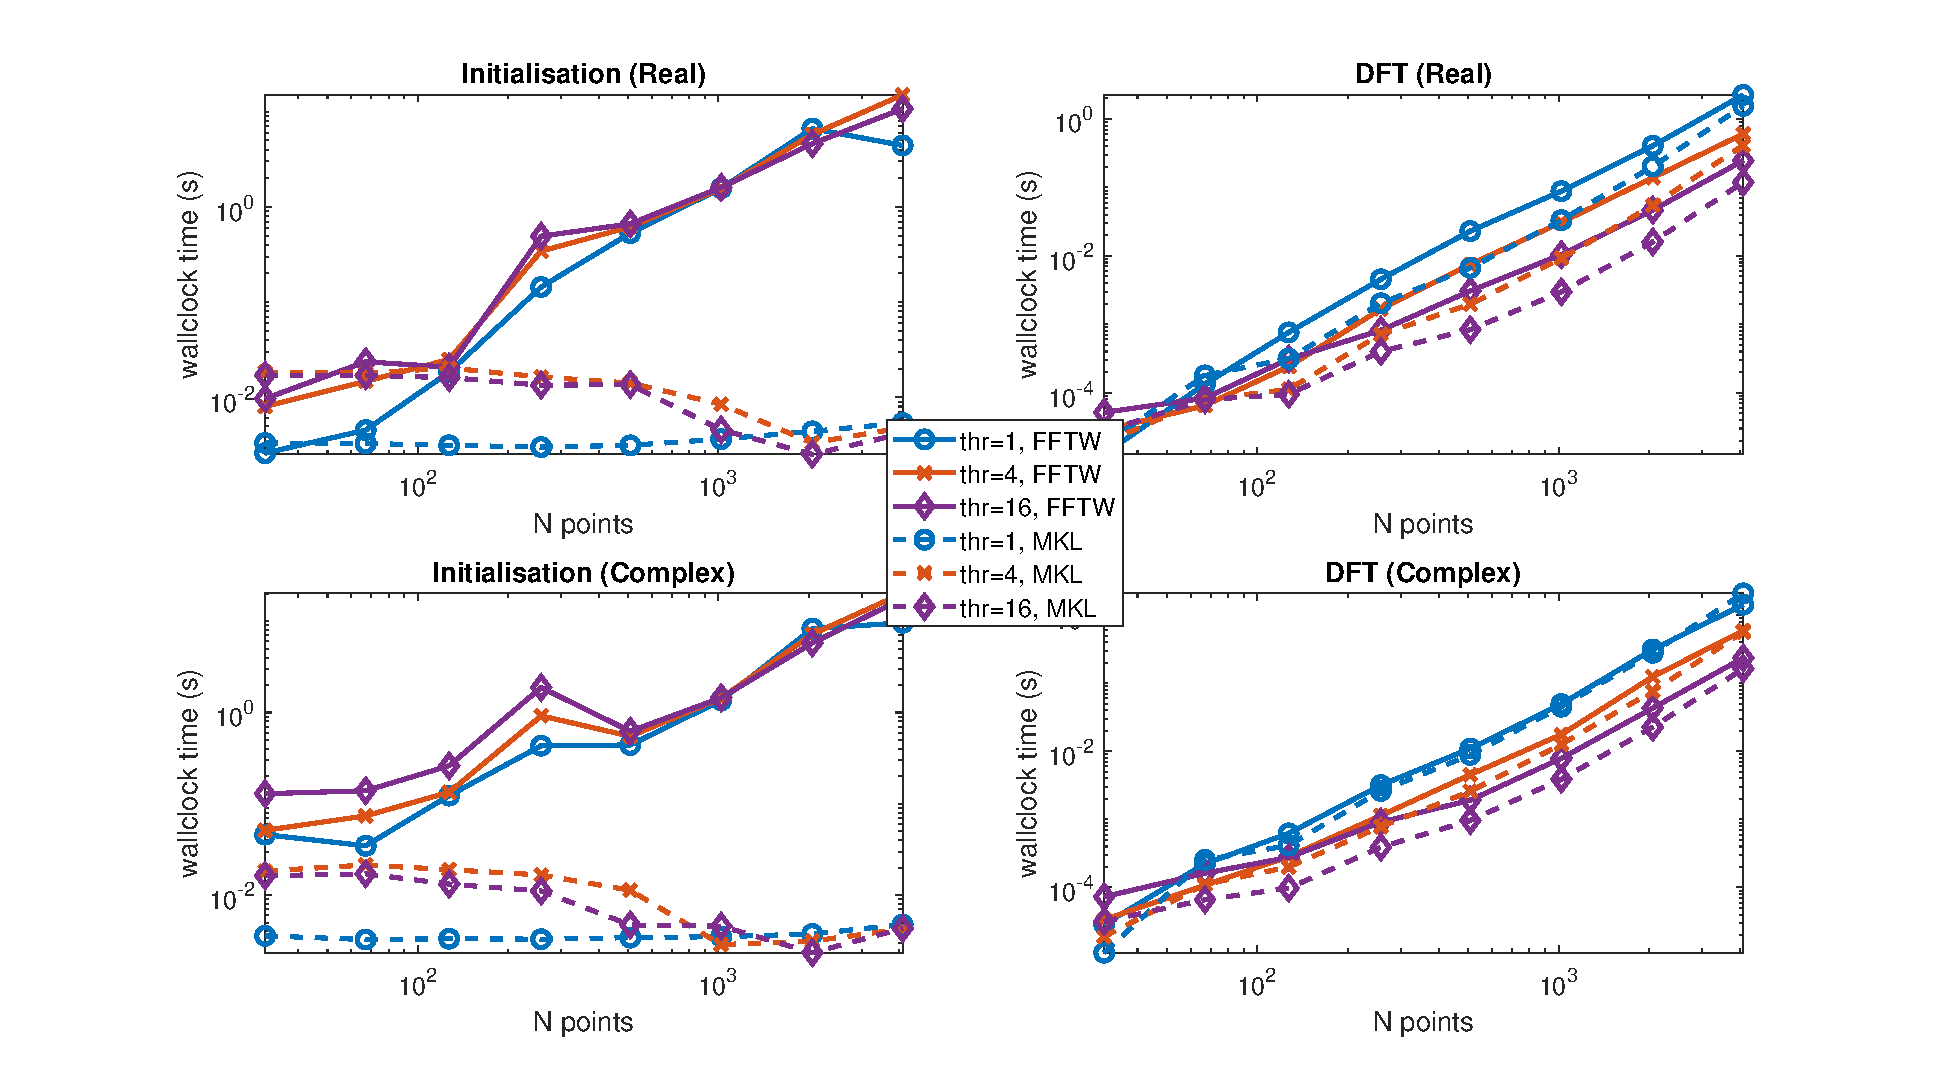
\includegraphics[width=\linewidth]{../results/fftw_mkl_prime_2d_thr.eps}
  \caption{Initialisation and DFT execution times of FFTW and MKL libraries applied to 2D signal as a function of the
    number of points, $N,$ and varying the number of threads, $thr.$ $N$ is a prime number.}
  \label{2DFFTWMKLPrime}
\end{figure}





\section{3D Multithreaded Benchmark Results}\label{Sec:3DMulti}


\subsection{3D FFTW Library}\label{Sec:3DFFTW}




\begin{figure}[htb]
    \centering
    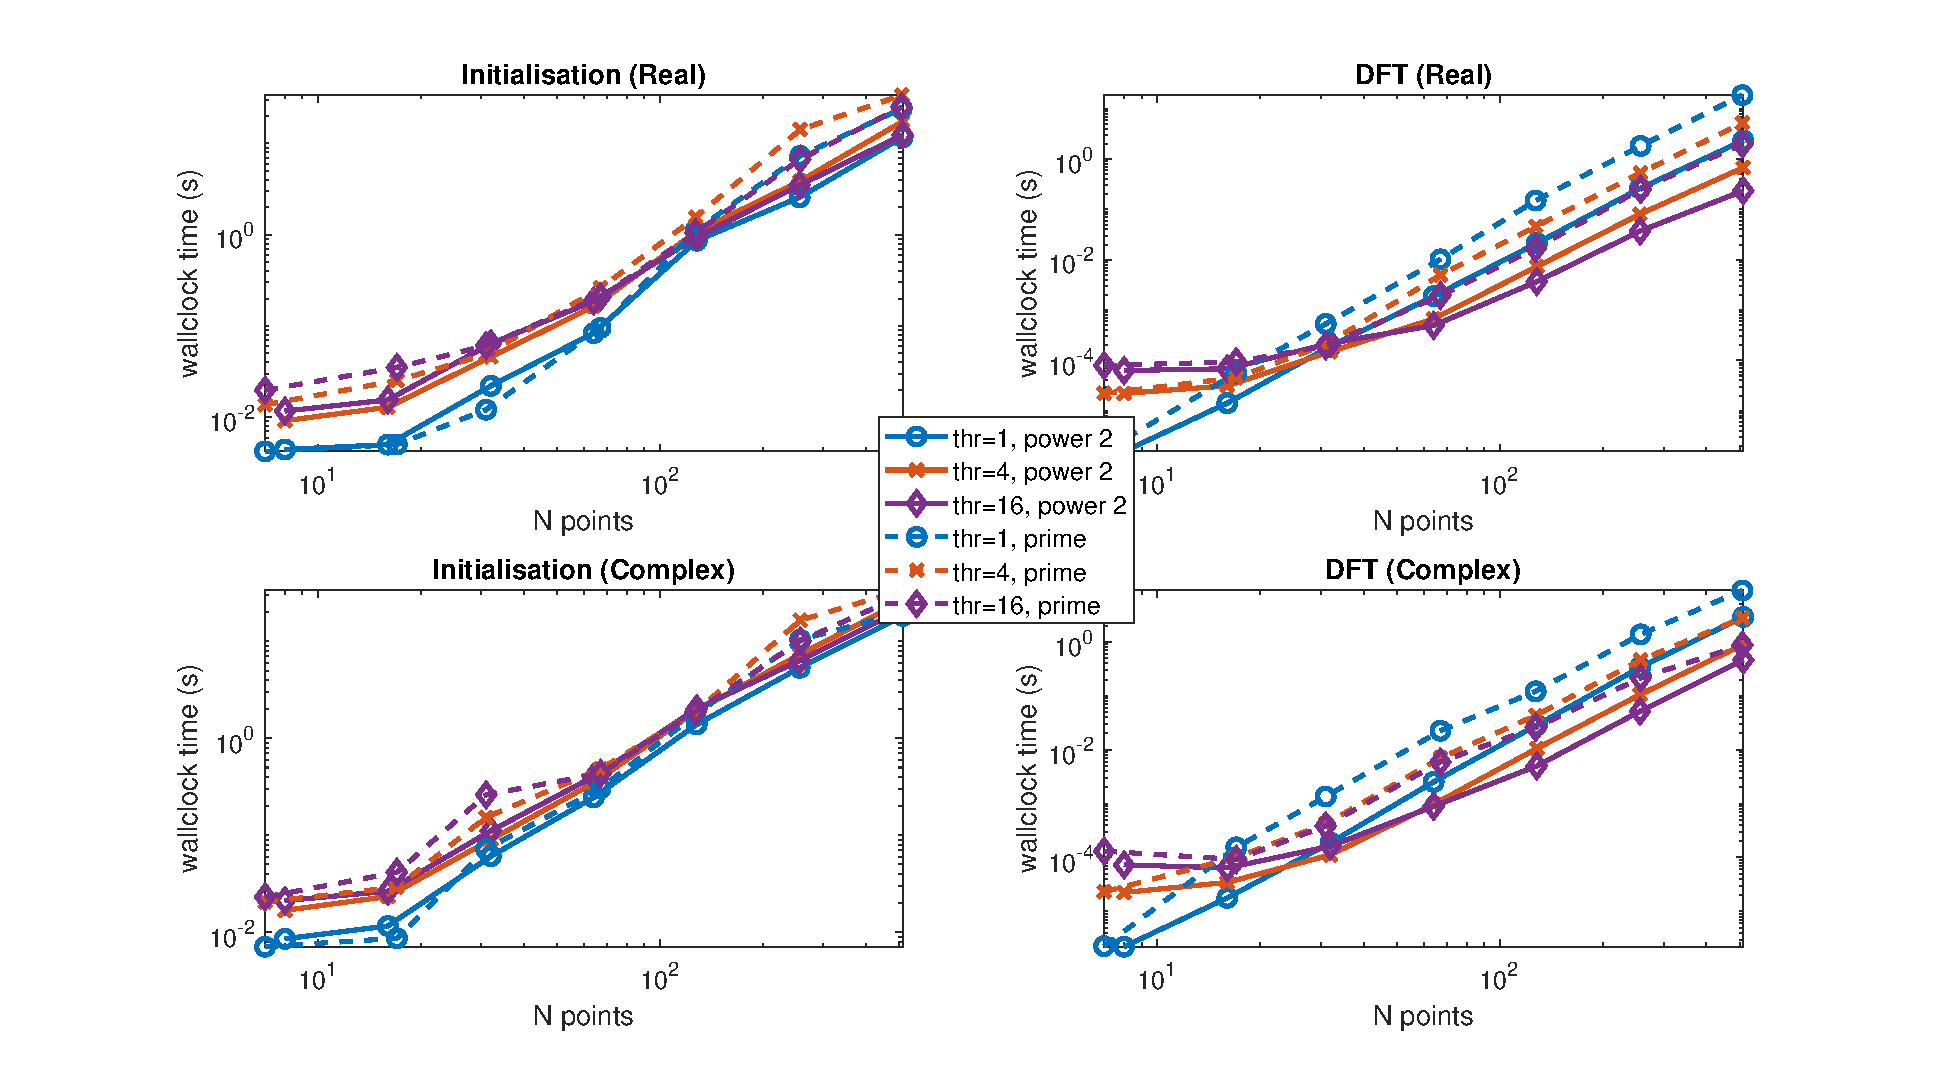
\includegraphics[width=\linewidth]{../results/fftw_3d_thr.eps}
  \caption{Initialisation and DFT execution times of FFTW library applied to 3D signal as a function of the
    number of points, $N,$ and varying the number of threads, $thr.$ }
  \label{3DFFTW}
\end{figure}

\subsection{3D MKL Library}\label{Sec:3DMKL}




\begin{figure}[htb]
    \centering
    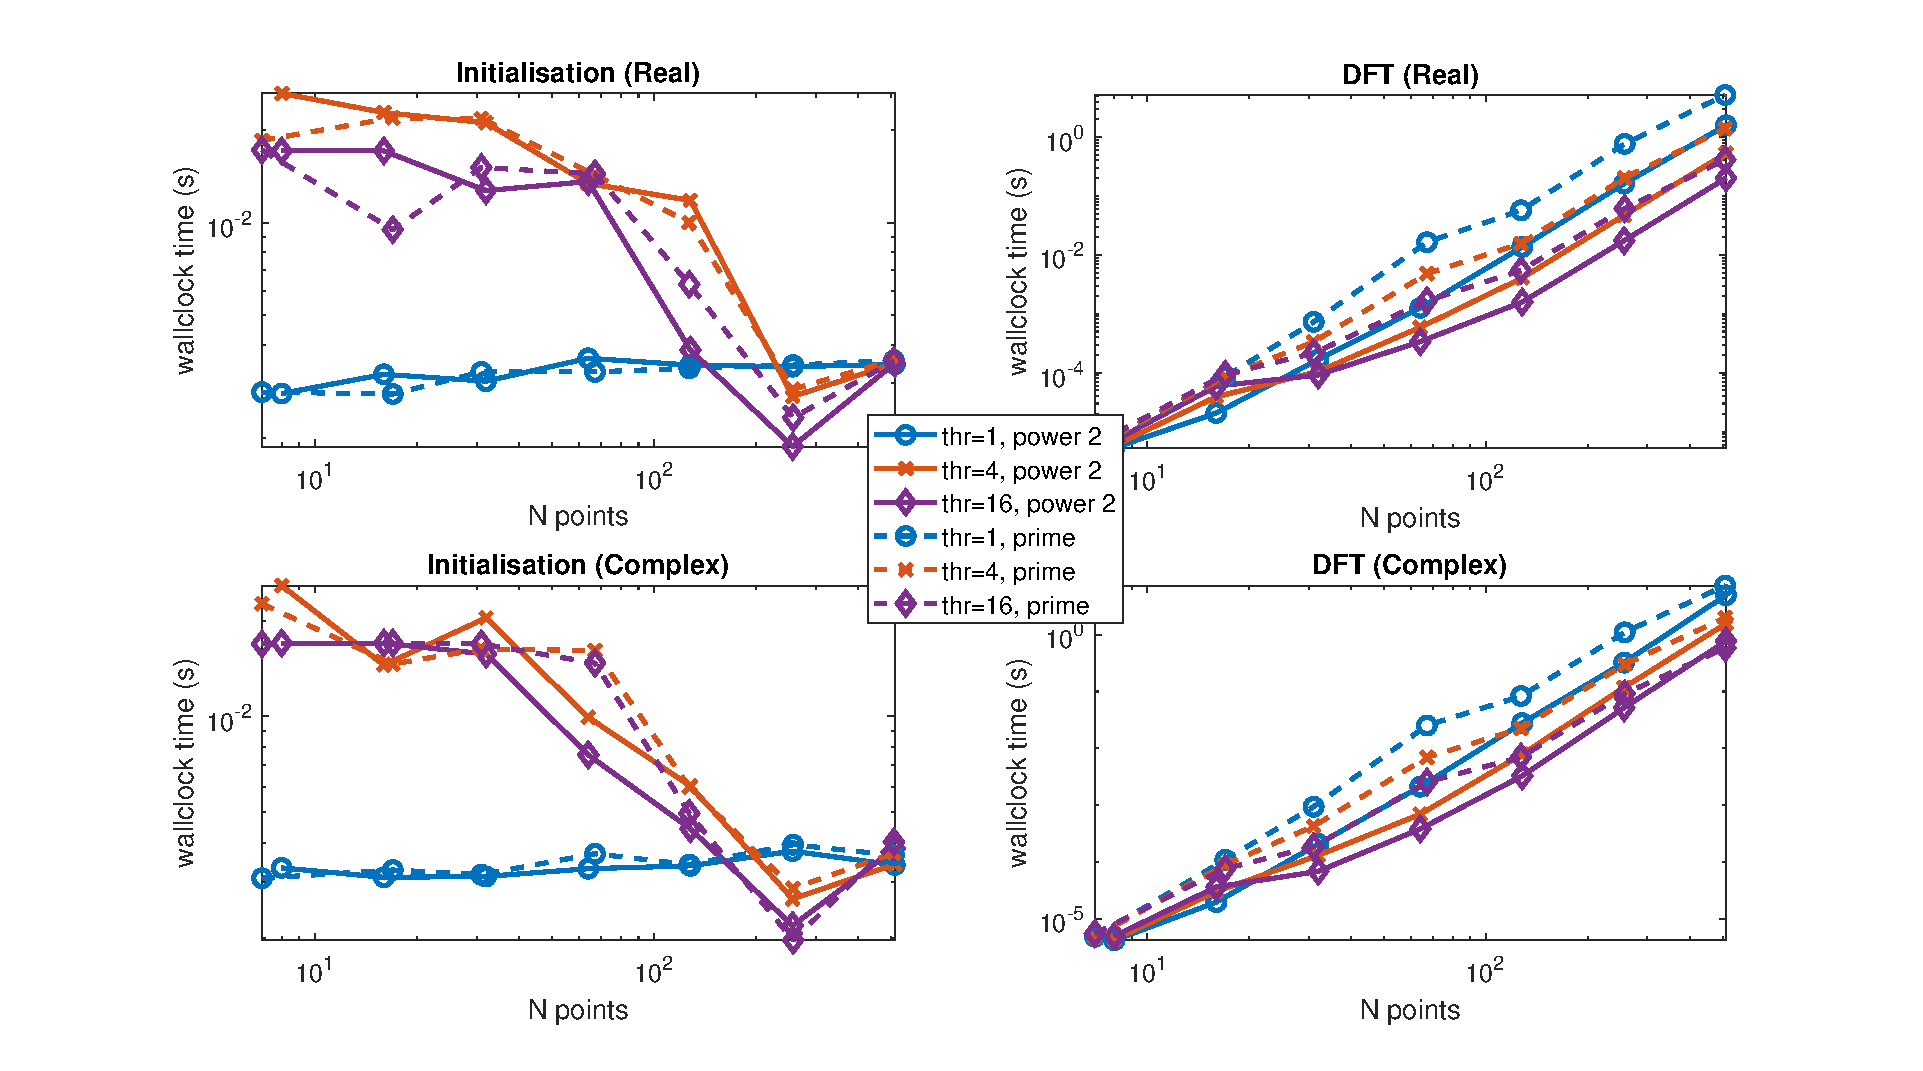
\includegraphics[width=\linewidth]{../results/mkl_3d_thr.eps}
  \caption{Initialisation and DFT execution times of MKL library applied to 3D signal as a function of the
    number of points, $N,$ and varying the number of threads, $thr.$ }
  \label{3DMKL}
\end{figure}



\subsection{3D P3DFFT Library}\label{Sec:3DP3DFFT}




\begin{figure}[htb]
    \centering
    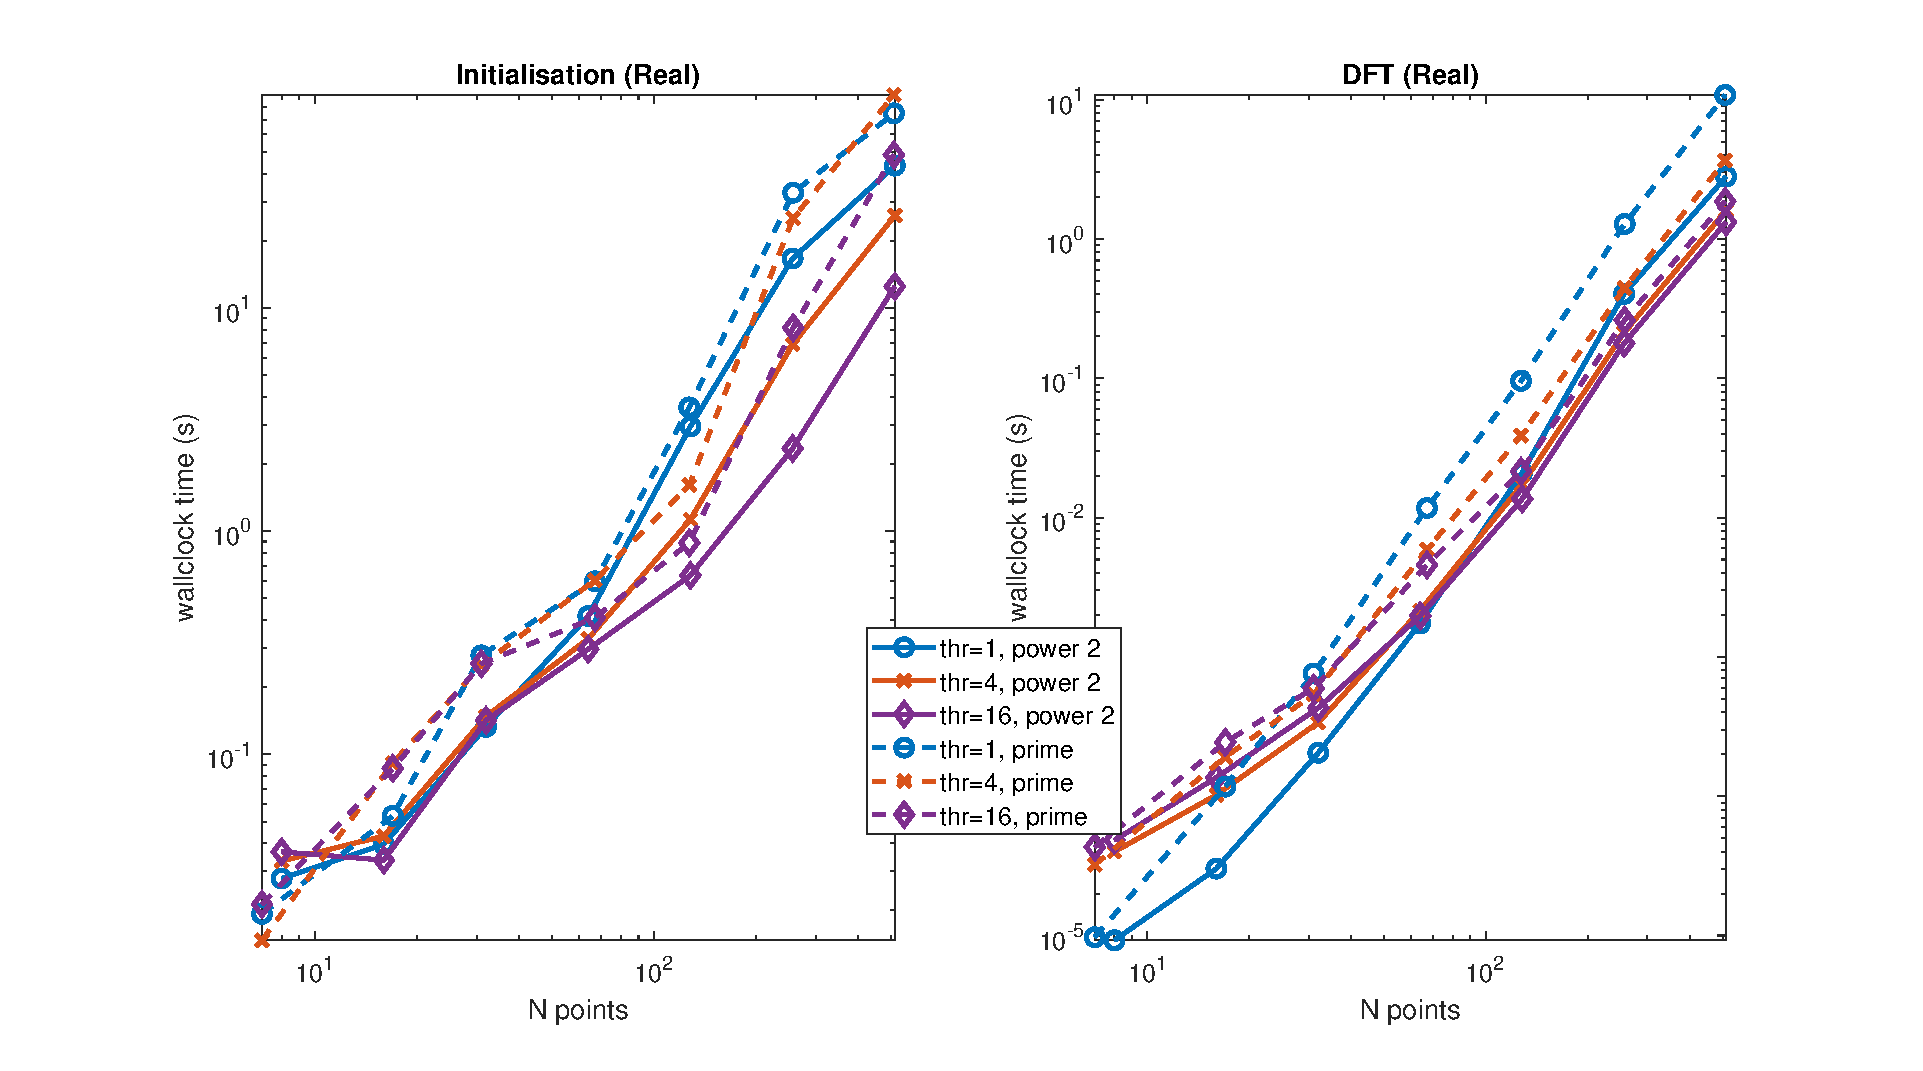
\includegraphics[width=\linewidth]{../results/p3dfft_3d_thr.eps}
  \caption{Initialisation and DFT execution times of MKL library applied to 3D signal as a function of the
    number of points, $N,$ and varying the number of threads, $thr.$ }
  \label{3DP3DFFT}
\end{figure}


\subsection{Comparison of libraries for 3D benchmarks}\label{Sec:3DComp}




\begin{figure}[htb]
    \centering
    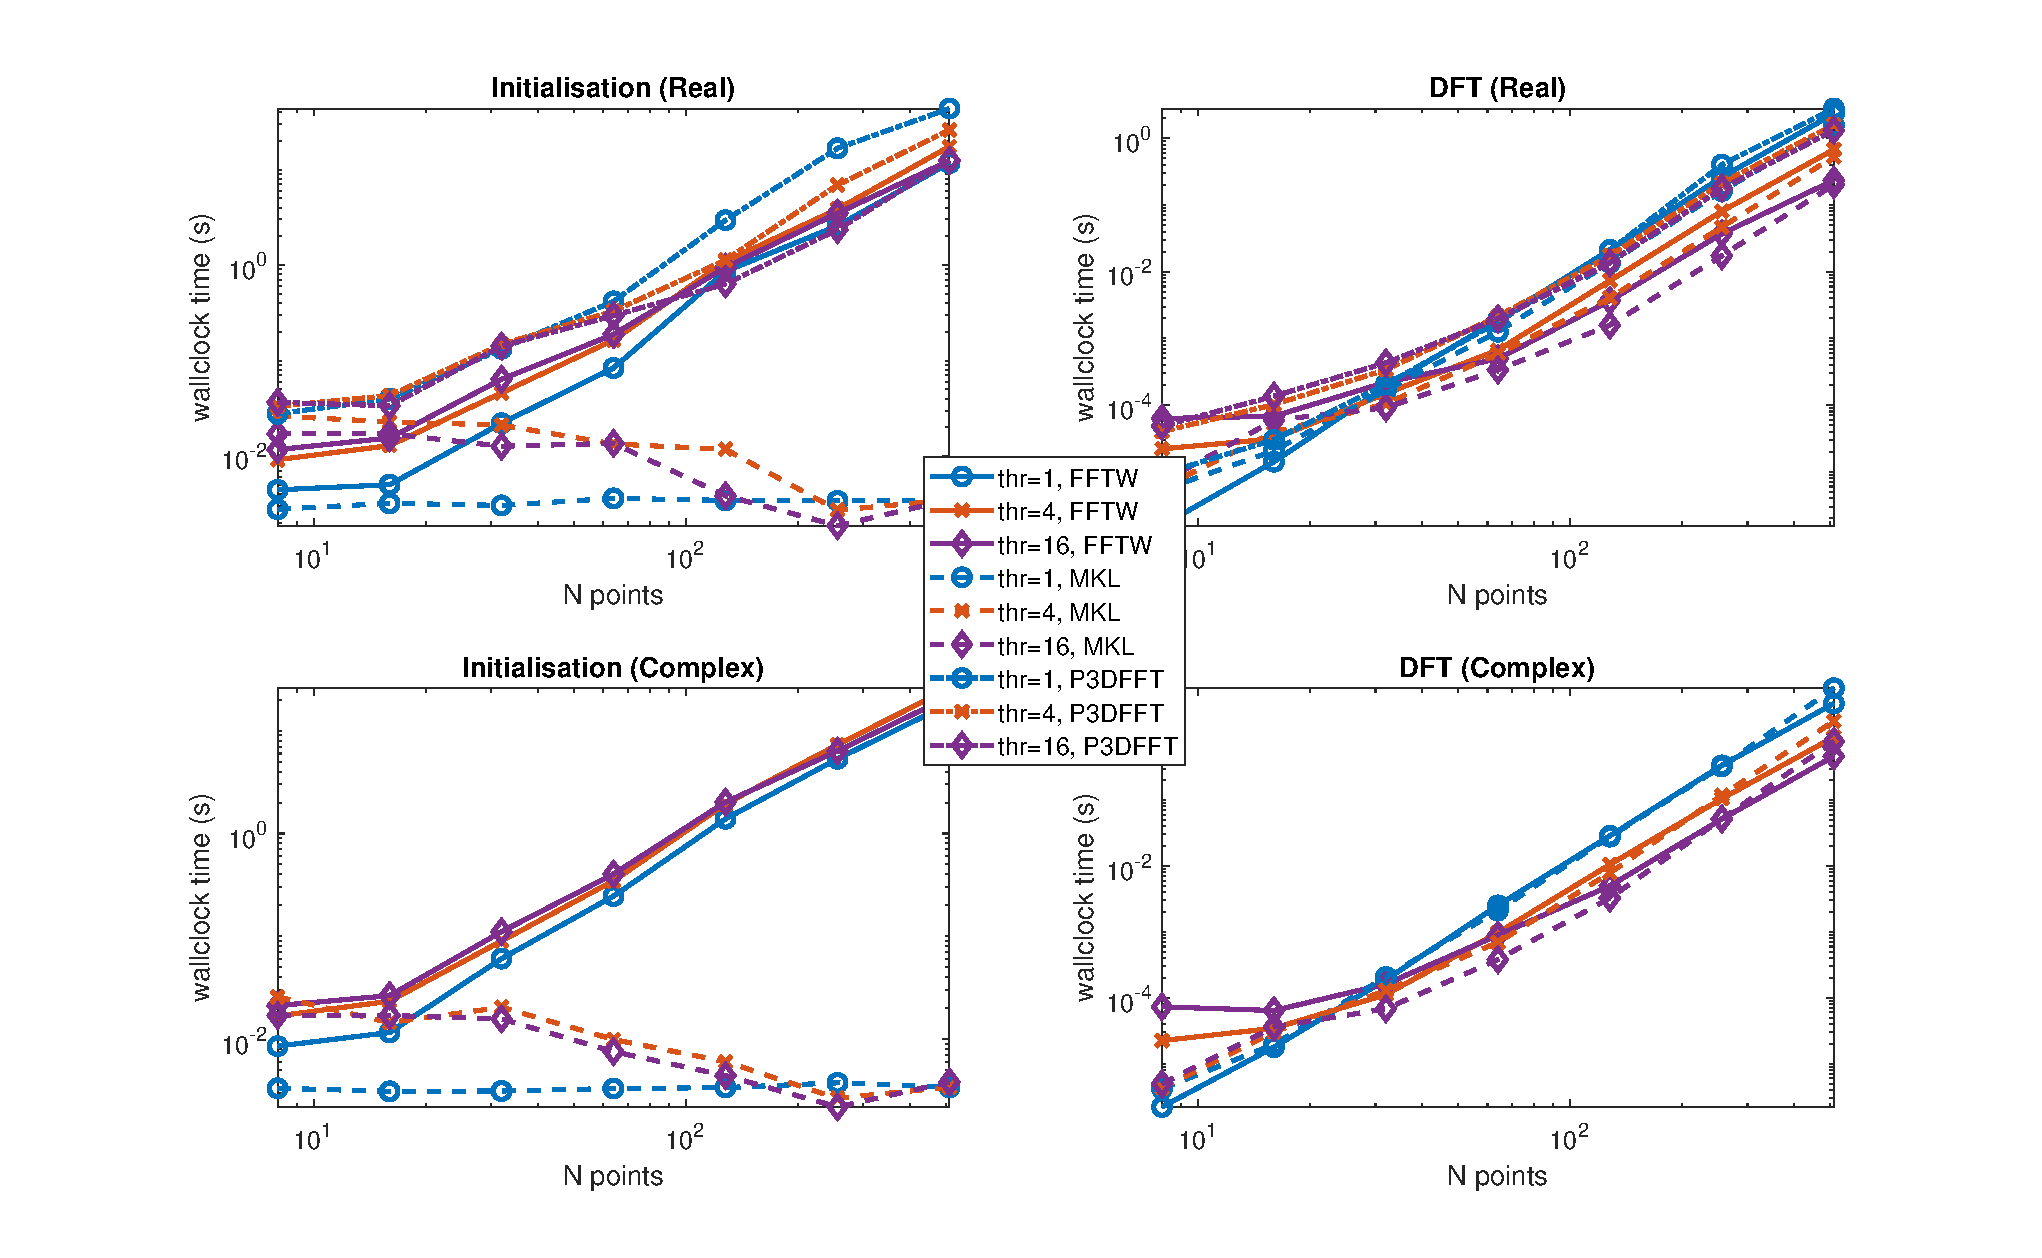
\includegraphics[width=\linewidth]{../results/fftw_mkl_p3dfft_2_3d_thr.eps}
  \caption{Initialisation and DFT execution times of FFTW, MKL and P3DFFT libraries applied to 3D signal as a function of the
    number of points, $N,$ and varying the number of threads, $thr.$ $N$ is a power of 2.}
  \label{3DFFTWMKL2}
\end{figure}


\begin{figure}[htb]
    \centering
    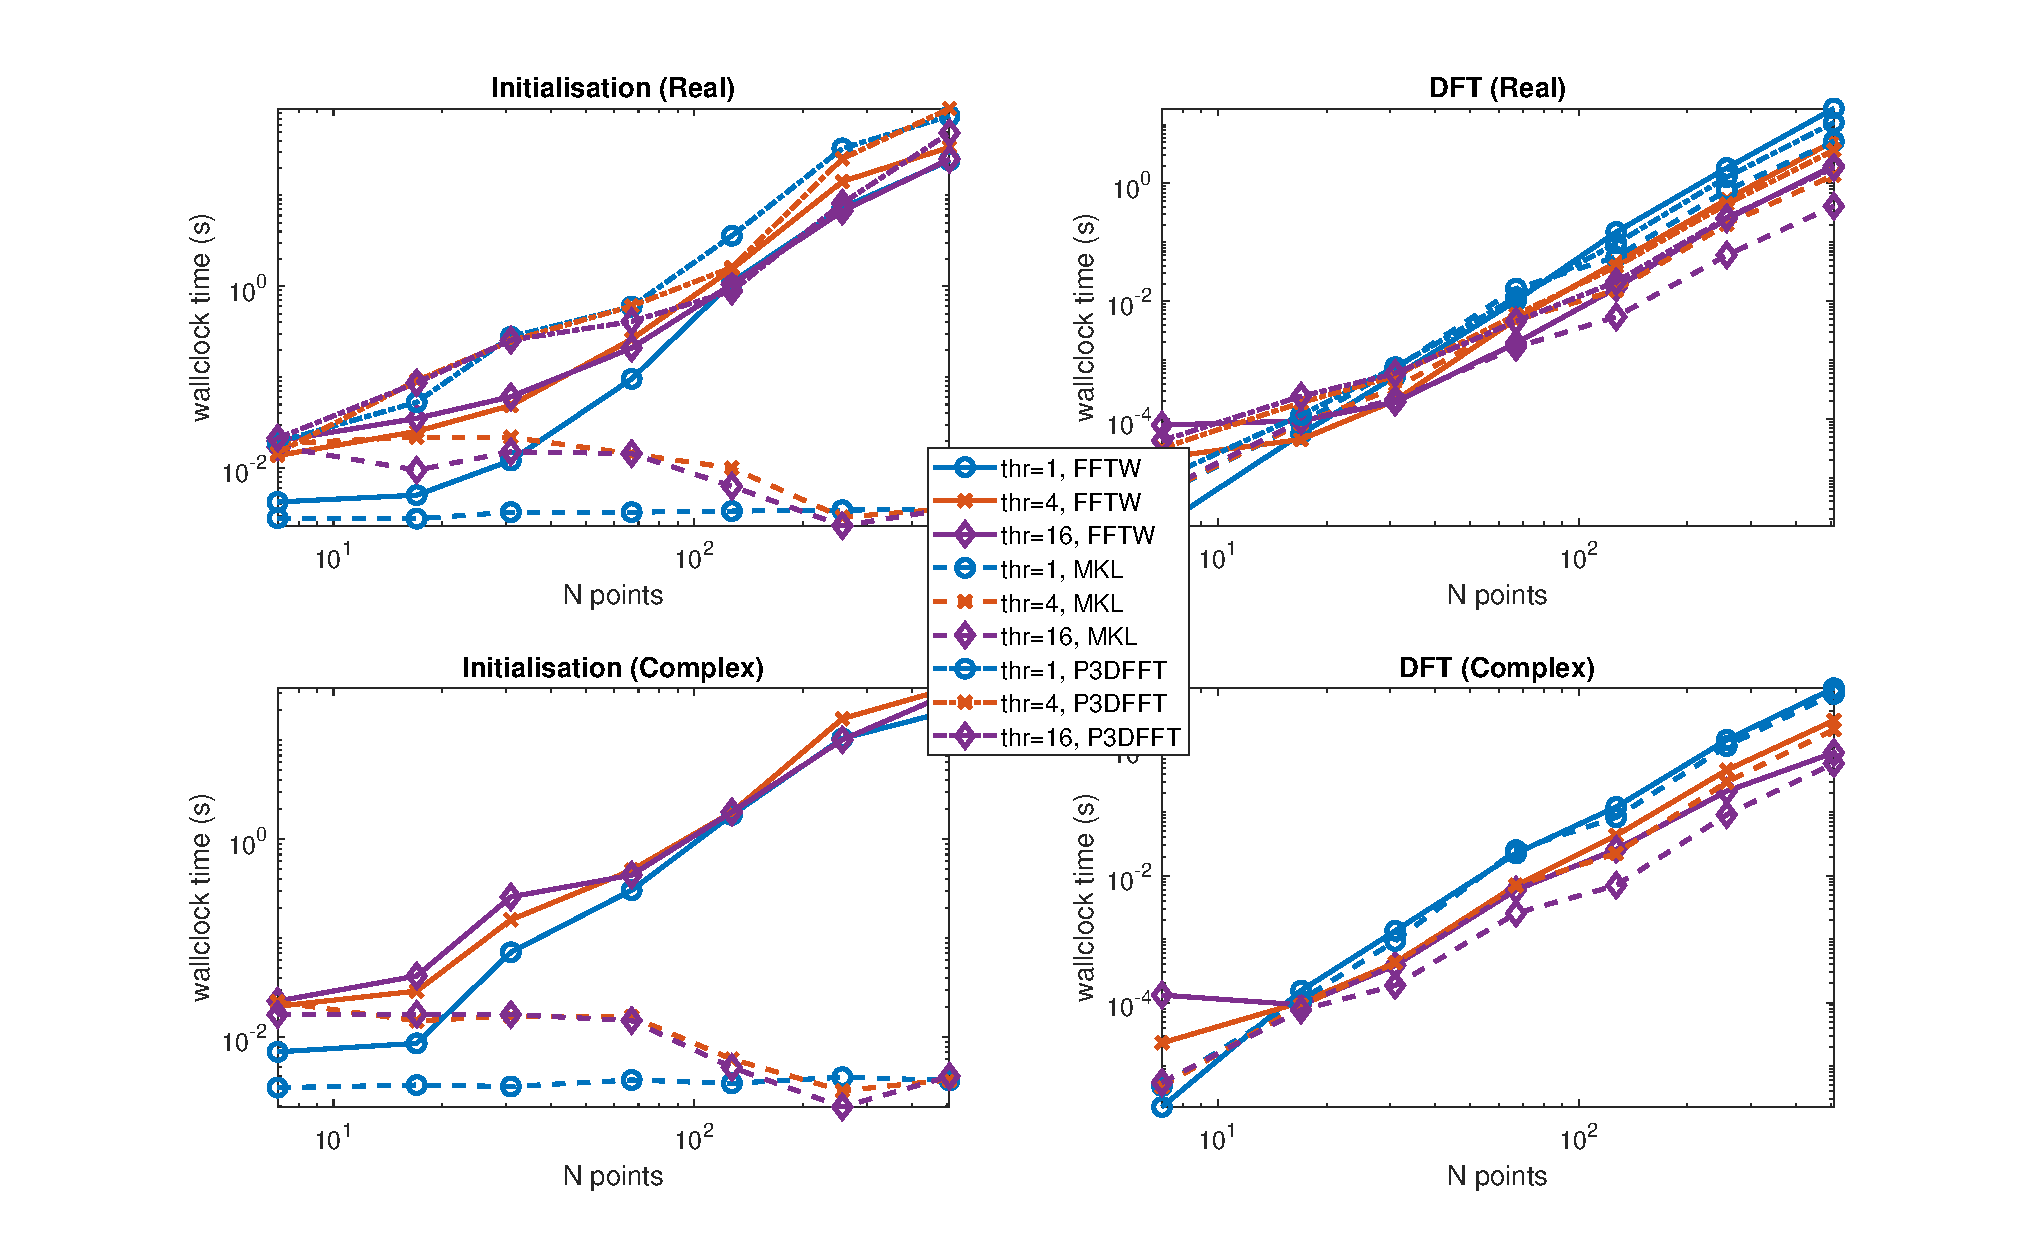
\includegraphics[width=\linewidth]{../results/fftw_mkl_p3dfft_prime_3d_thr.eps}
  \caption{Initialisation and DFT execution times of FFTW, MKL and P3DFFT libraries applied to 3D signal as a function of the
    number of points, $N,$ and varying the number of threads, $thr.$ $N$ is a prime number.}
  \label{3DFFTWMKLPrime}
\end{figure}




\section{1D Distributed Benchmark Results}\label{Sec:1DDistr}


\subsection{1D Distributed FFTW Library}\label{Sec:1DDistFFTW}

\begin{figure}[htb]
    \centering
    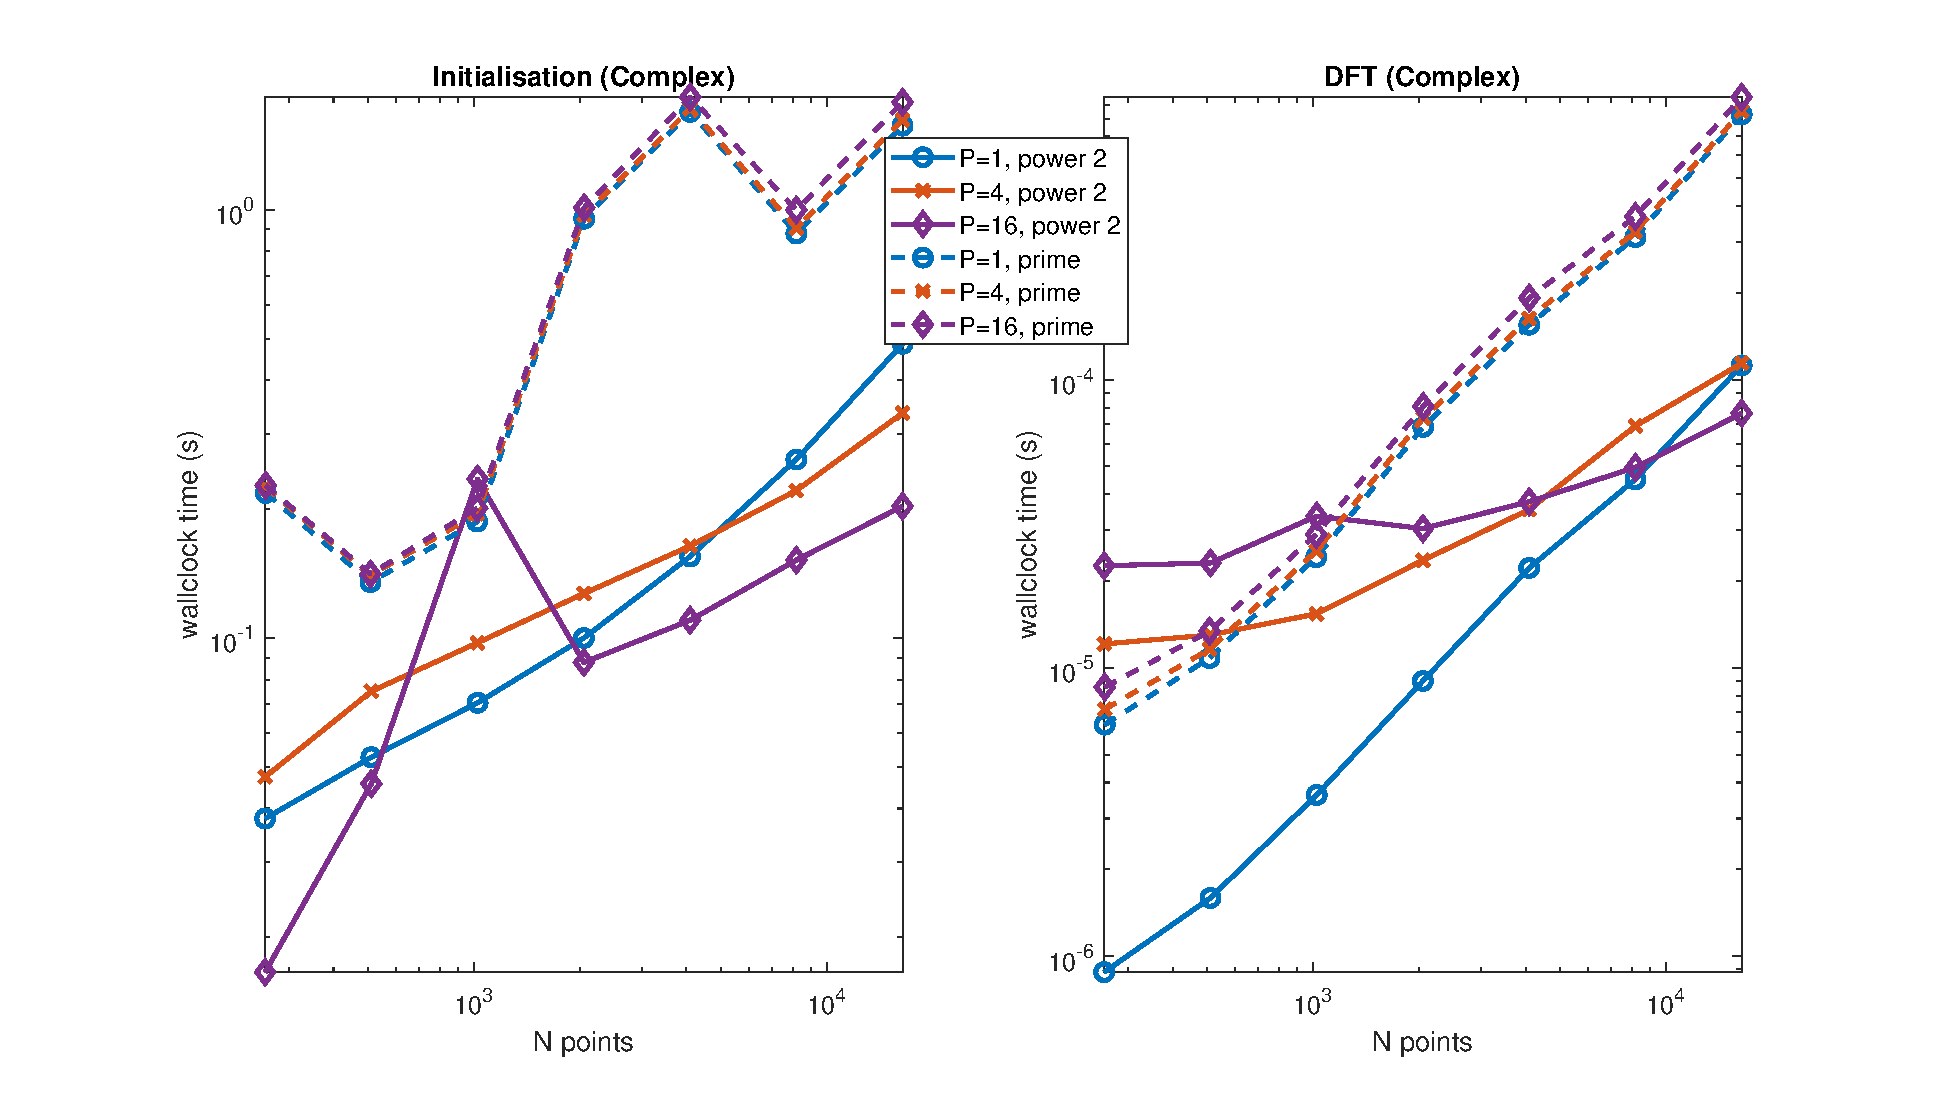
\includegraphics[width=\linewidth]{../results/fftw_1d_mpi.eps}
  \caption{Initialisation and DFT execution times of distributed FFTW library applied to 1D signal as a function of the
    number of points, $N,$ and varying the number of MPI processes, $P,$ with one thread per process.}
  \label{1DDistFFTW}
\end{figure}

\begin{figure}[htb]
    \centering
    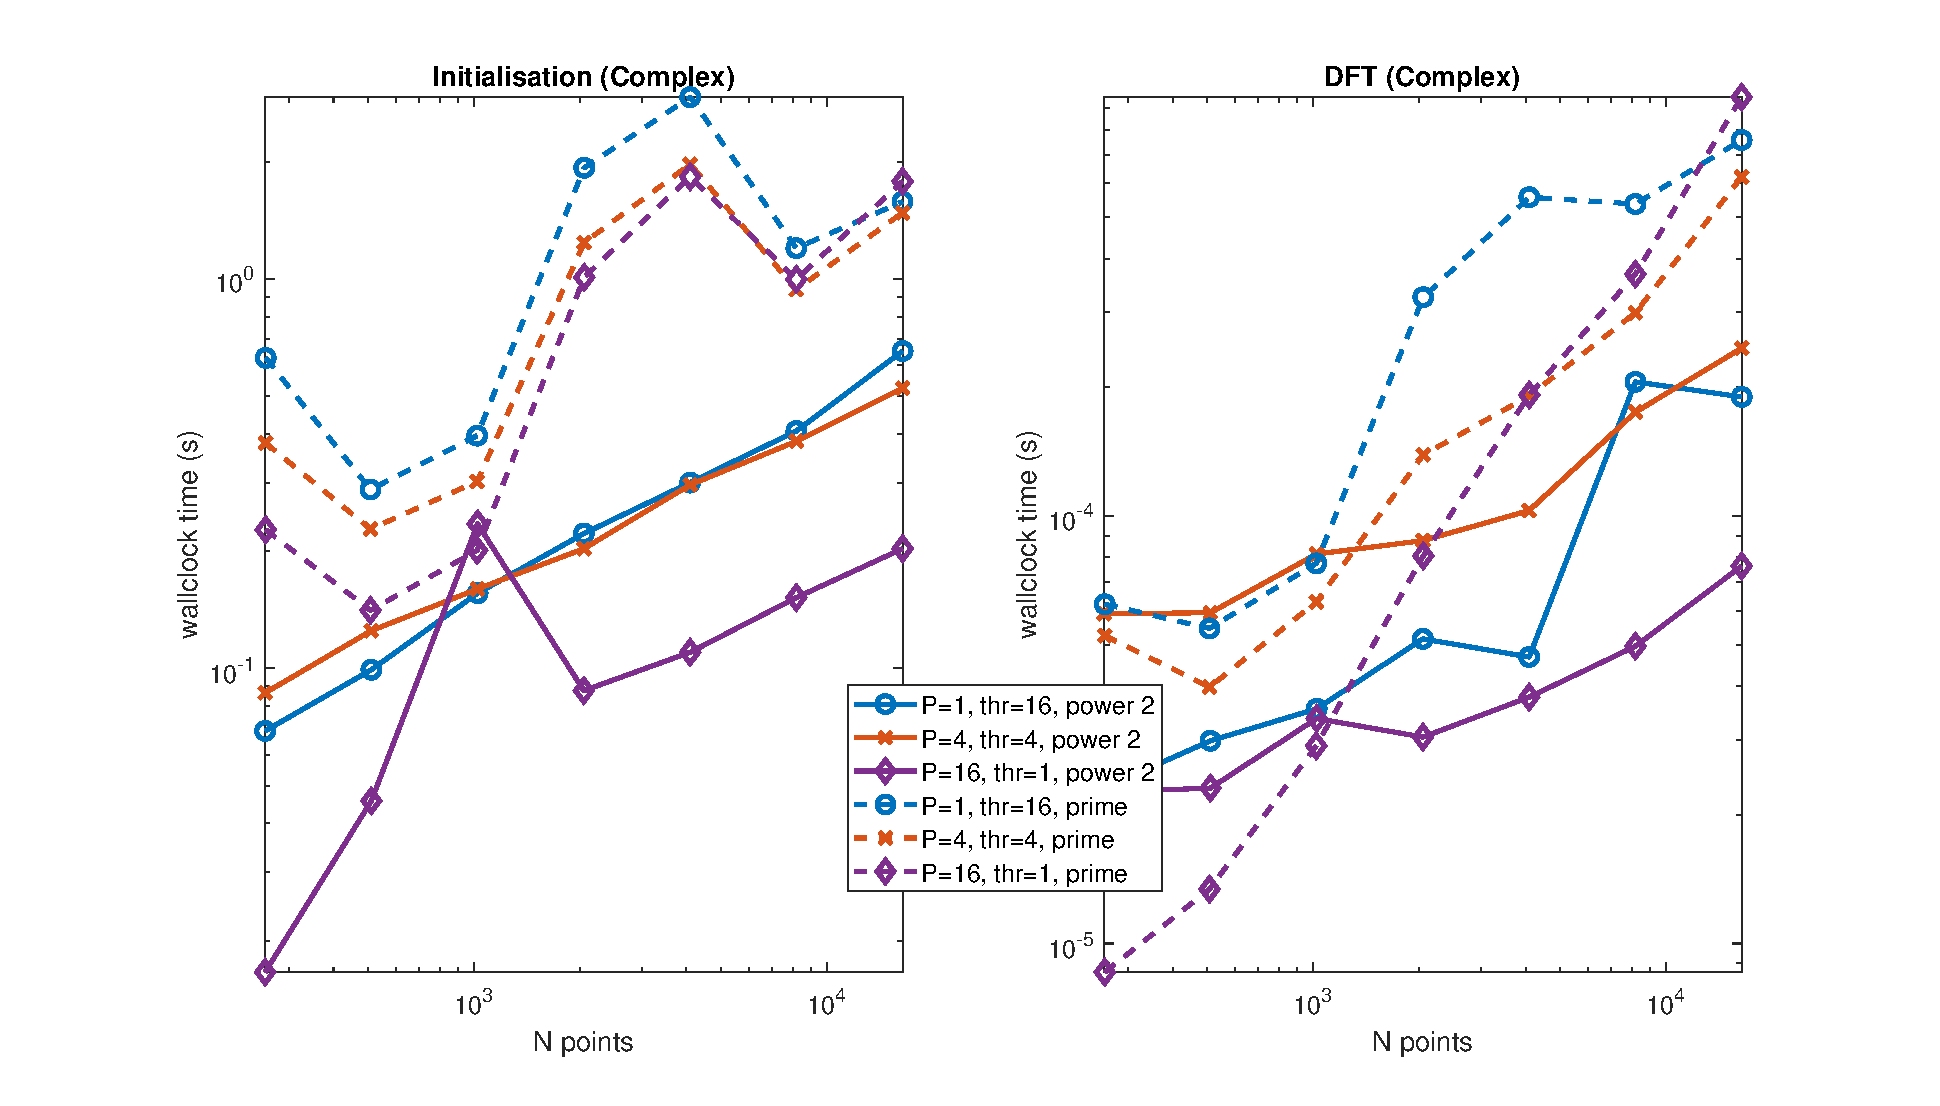
\includegraphics[width=\linewidth]{../results/fftw_1d_mpi_thr.eps}
  \caption{Initialisation and DFT execution times of distributed FFTW library applied to 1D signal as a function of the
    number of points, $N,$ and varying the number of MPI processes, $P,$ and threads, $thr,$ whilst maintaining $P\times thr=16.$}
  \label{1DDistFFTW16}
\end{figure}



\subsection{1D Distributed MKL Library}\label{Sec:1DDistMKL}

\begin{figure}[htb]
    \centering
    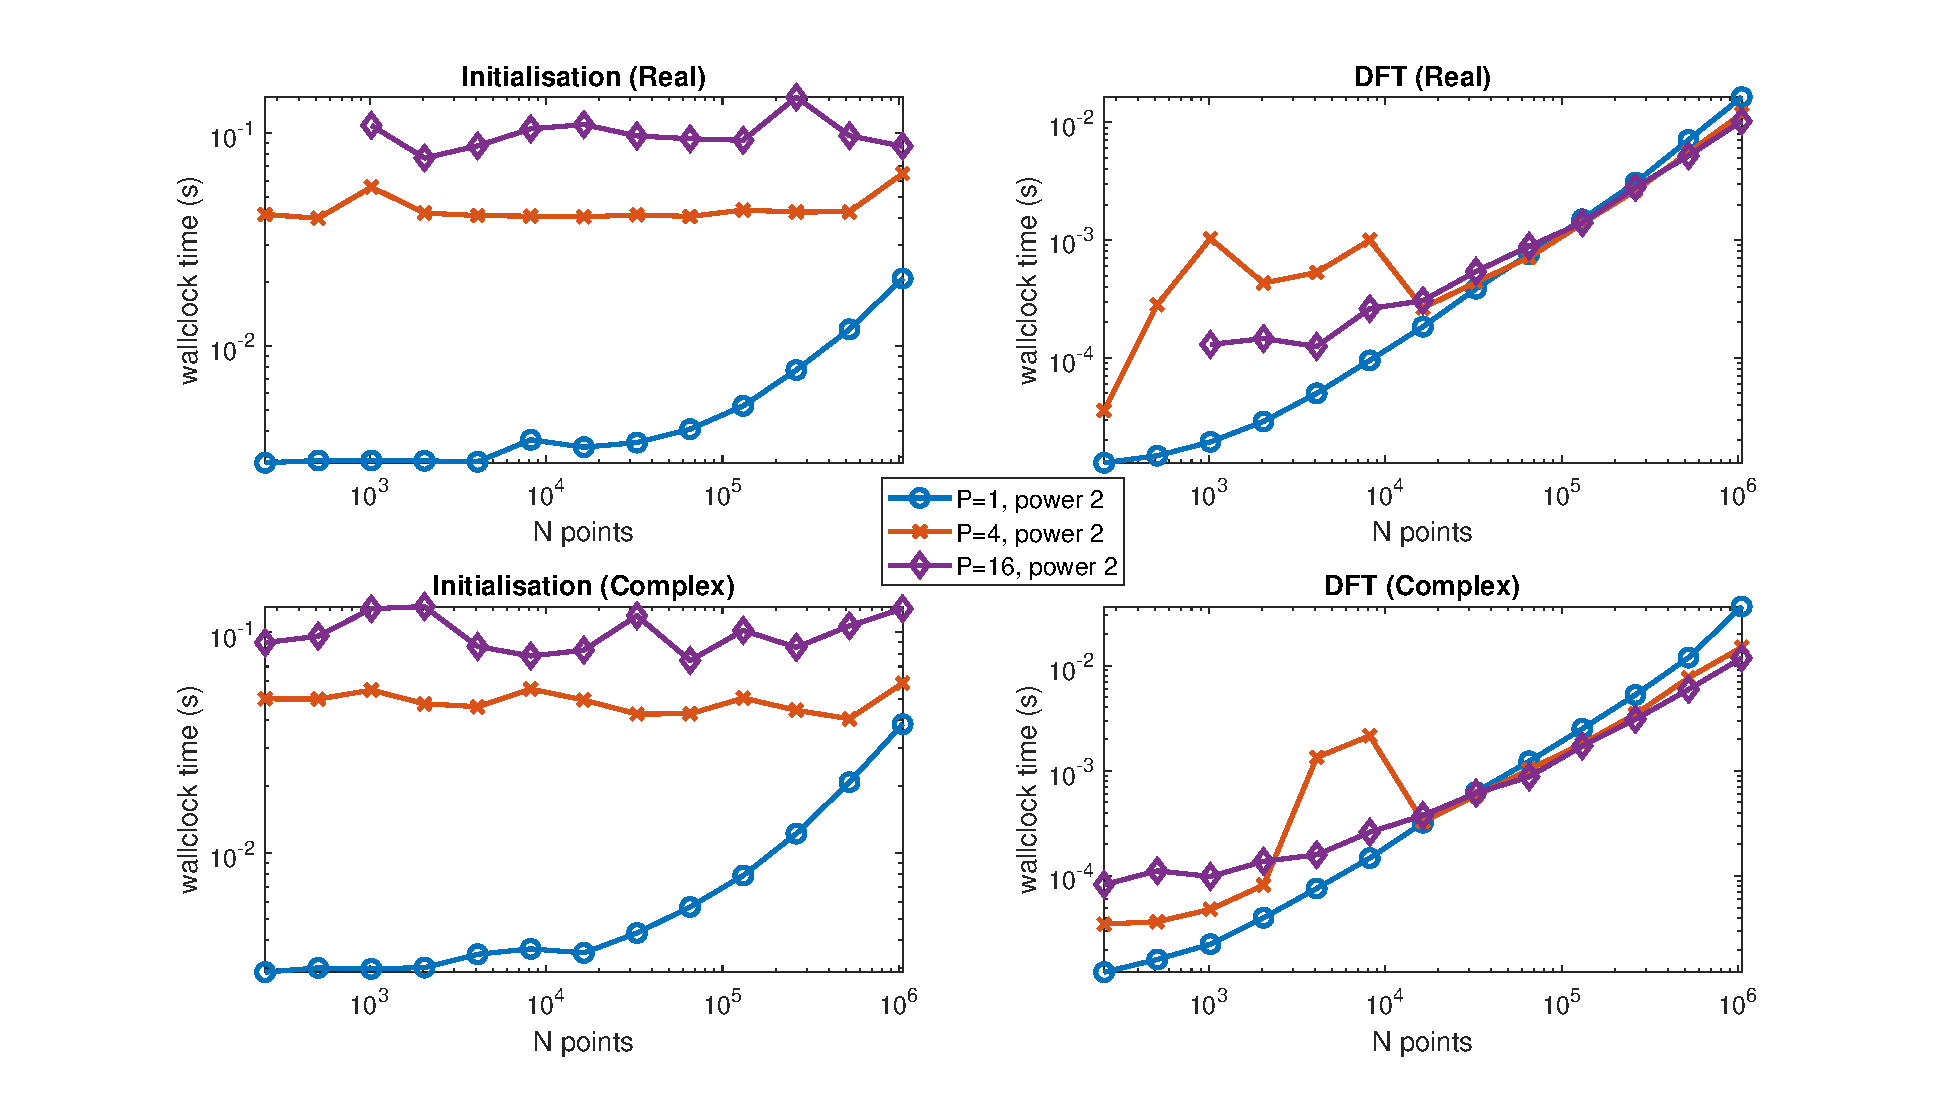
\includegraphics[width=\linewidth]{../results/mkl_1d_mpi.eps}
  \caption{Initialisation and DFT execution times of distributed MKL library applied to 1D signal as a function of the
    number of points, $N,$ and varying the number of MPI processes, $P,$ with one thread per process.}
  \label{1DDistMKL}
\end{figure}

\begin{figure}[htb]
    \centering
    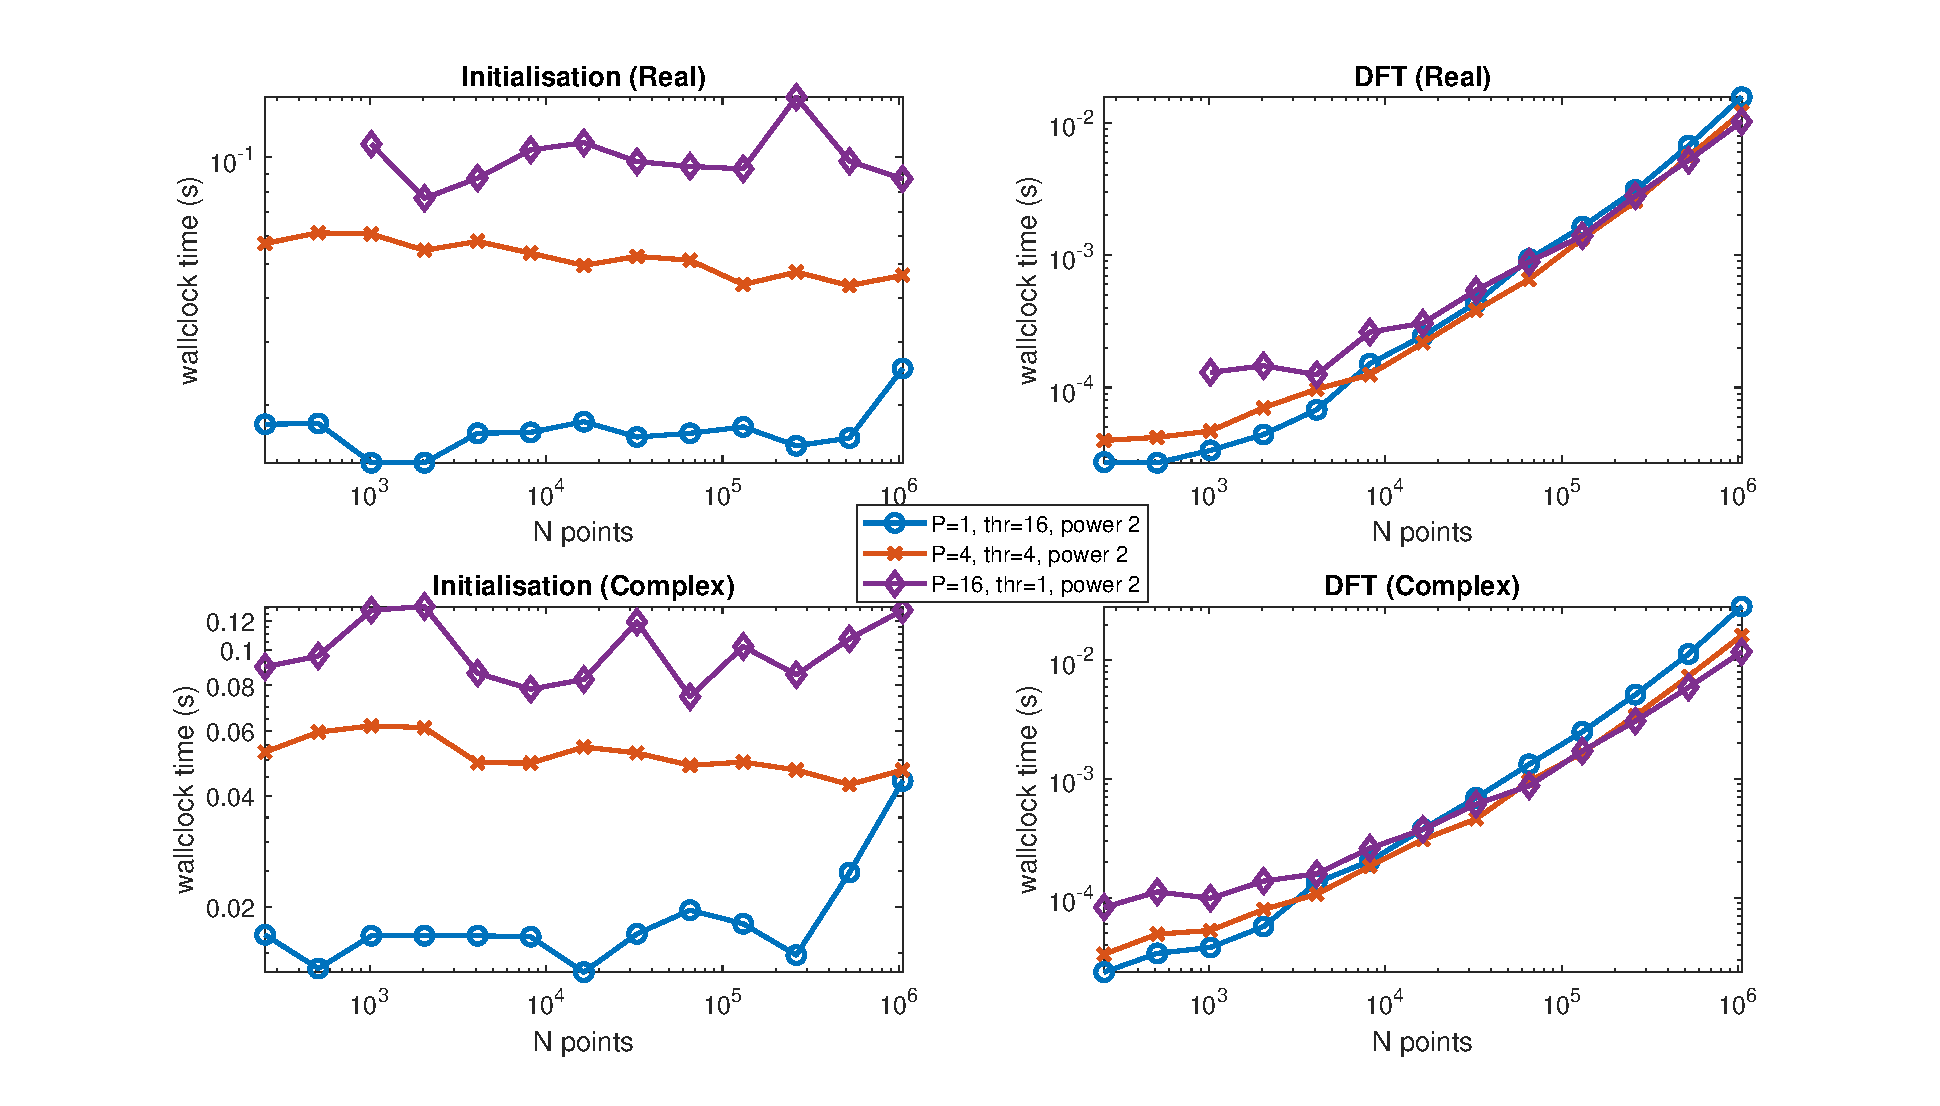
\includegraphics[width=\linewidth]{../results/mkl_1d_mpi_thr.eps}
  \caption{Initialisation and DFT execution times of distributed MKL library applied to 1D signal as a function of the
    number of points, $N,$ and varying the number of MPI processes, $P,$ and threads, $thr,$ whilst maintaining $P\times thr=16.$}
  \label{1DDistMKL16}
\end{figure}

\subsection{Comparison of distributed libraries for 1D benchmark}\label{Sec:1DDistComp}


\begin{figure}[htb]
    \centering
    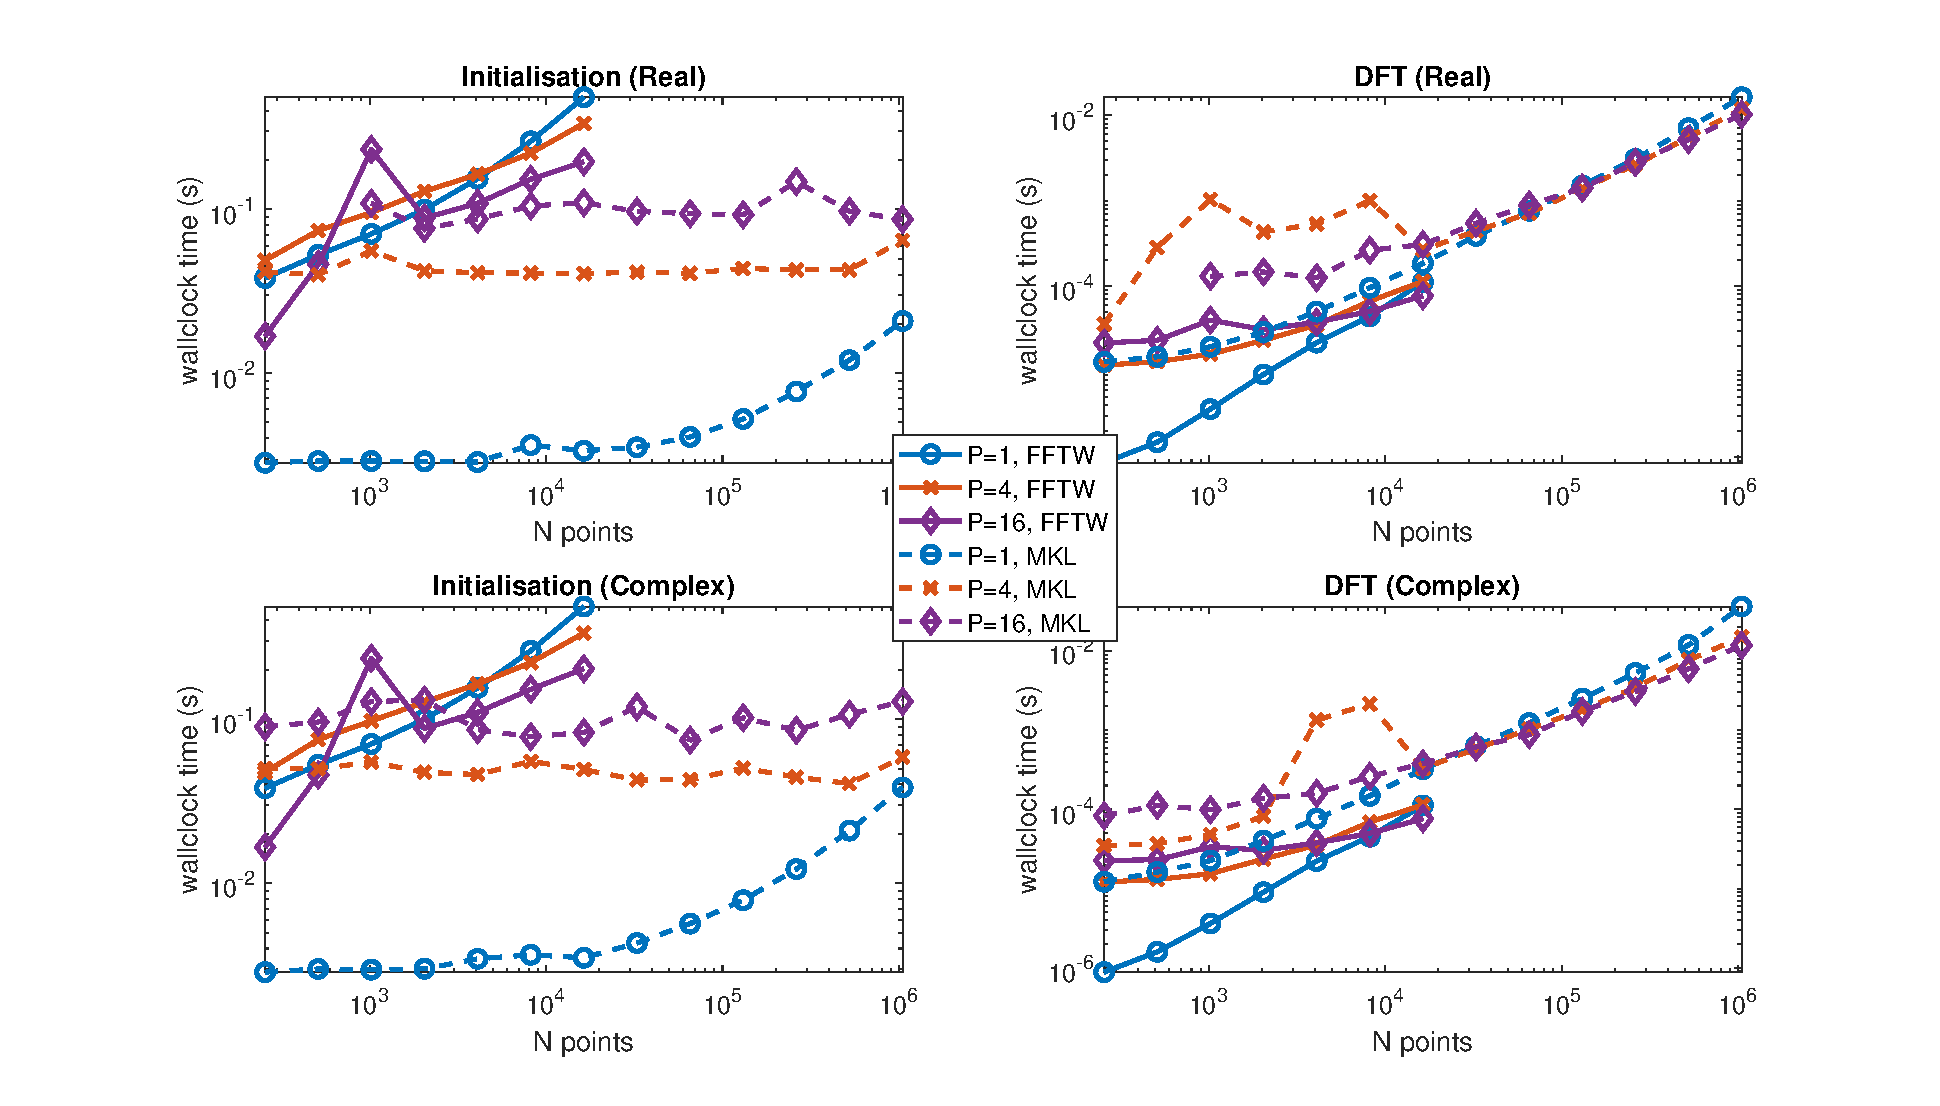
\includegraphics[width=\linewidth]{../results/fftw_mkl_2_1d_mpi.eps}
  \caption{Initialisation and DFT execution times of distributed FFTW and MKL libraries applied to 1D signal as a function of the
    number of points, $N,$ and varying the number of MPI processes, $P,$ with one thread per process. $N$ is a power of 2.}
  \label{1DDistFFTWMKL2}
\end{figure}


No prime comparison because MKL doesn't do prime N. Real values for FFTW were reals converted to complex values.


\section{2D Distributed Benchmark Results}\label{Sec:2DDistr}

\subsection{2D Distributed FFTW Library}\label{Sec:2DDistFFTW}

\begin{figure}[htb]
    \centering
    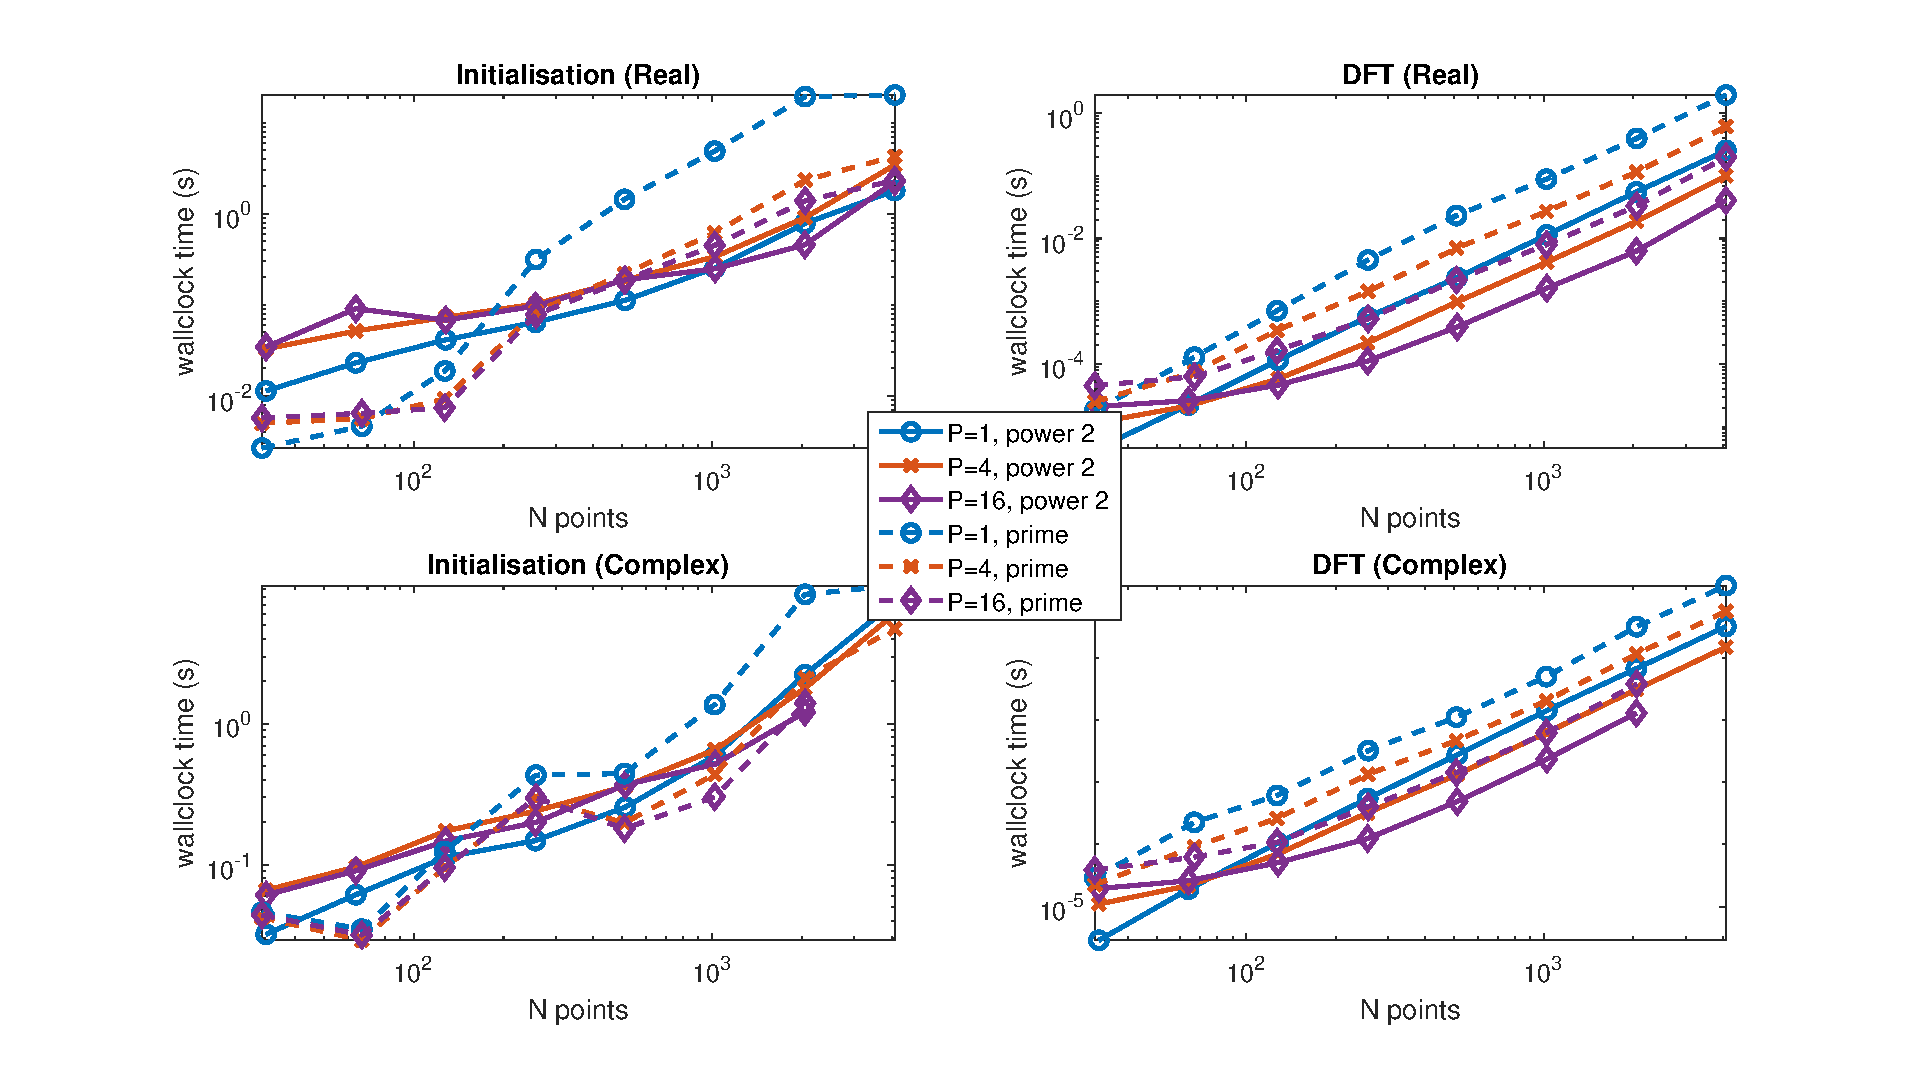
\includegraphics[width=\linewidth]{../results/fftw_2d_mpi.eps}
  \caption{Initialisation and DFT execution times of distributed FFTW library applied to 2D signal as a function of the
    number of points, $N,$ and varying the number of MPI processes, $P,$ with one thread per process.}
  \label{2DDistFFTW}
\end{figure}

\begin{figure}[htb]
    \centering
    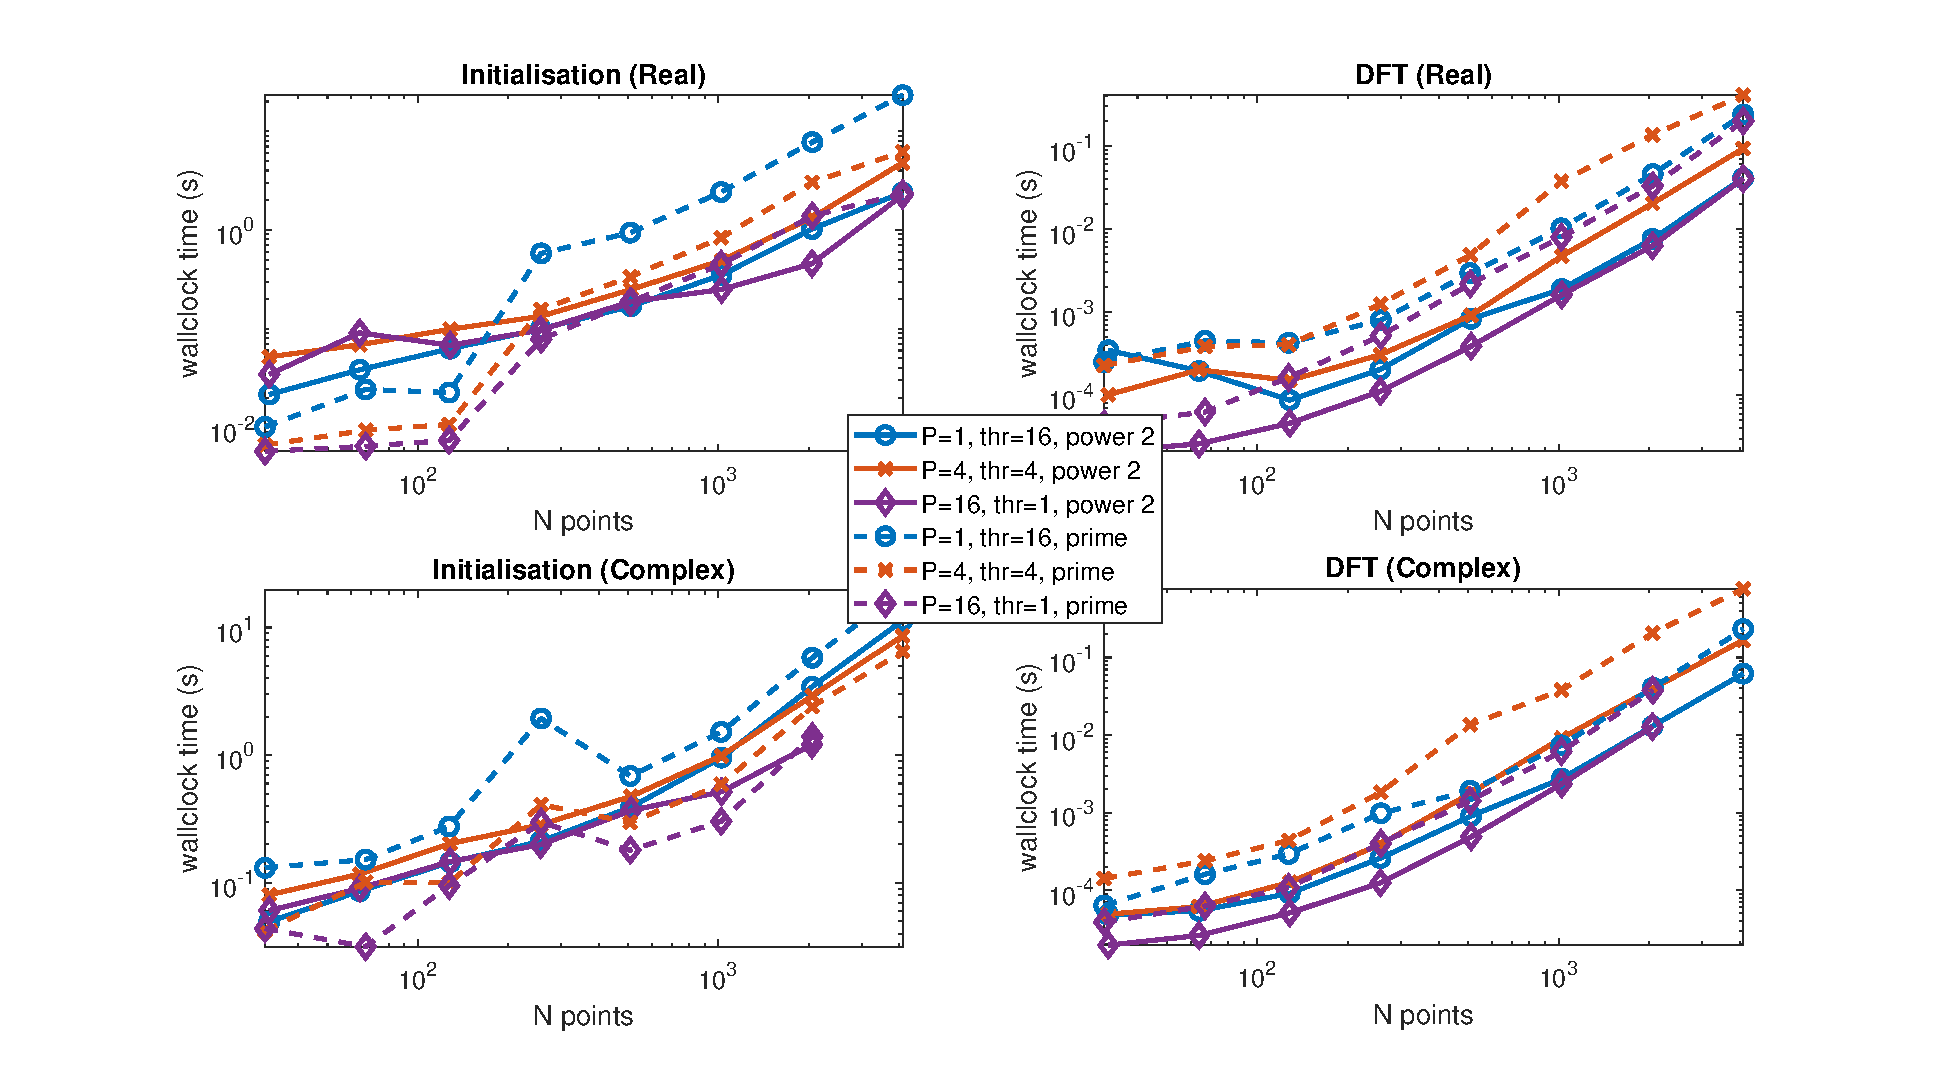
\includegraphics[width=\linewidth]{../results/fftw_2d_mpi_thr.eps}
  \caption{Initialisation and DFT execution times of distributed FFTW library applied to 2D signal as a function of the
    number of points, $N,$ and varying the number of MPI processes, $P,$ and threads, $thr,$ whilst maintaining $P\times thr=16.$}
  \label{2DDistFFTW16}
\end{figure}



\subsection{2D Distributed MKL Library}\label{Sec:2DDistMKL}

\begin{figure}[htb]
    \centering
    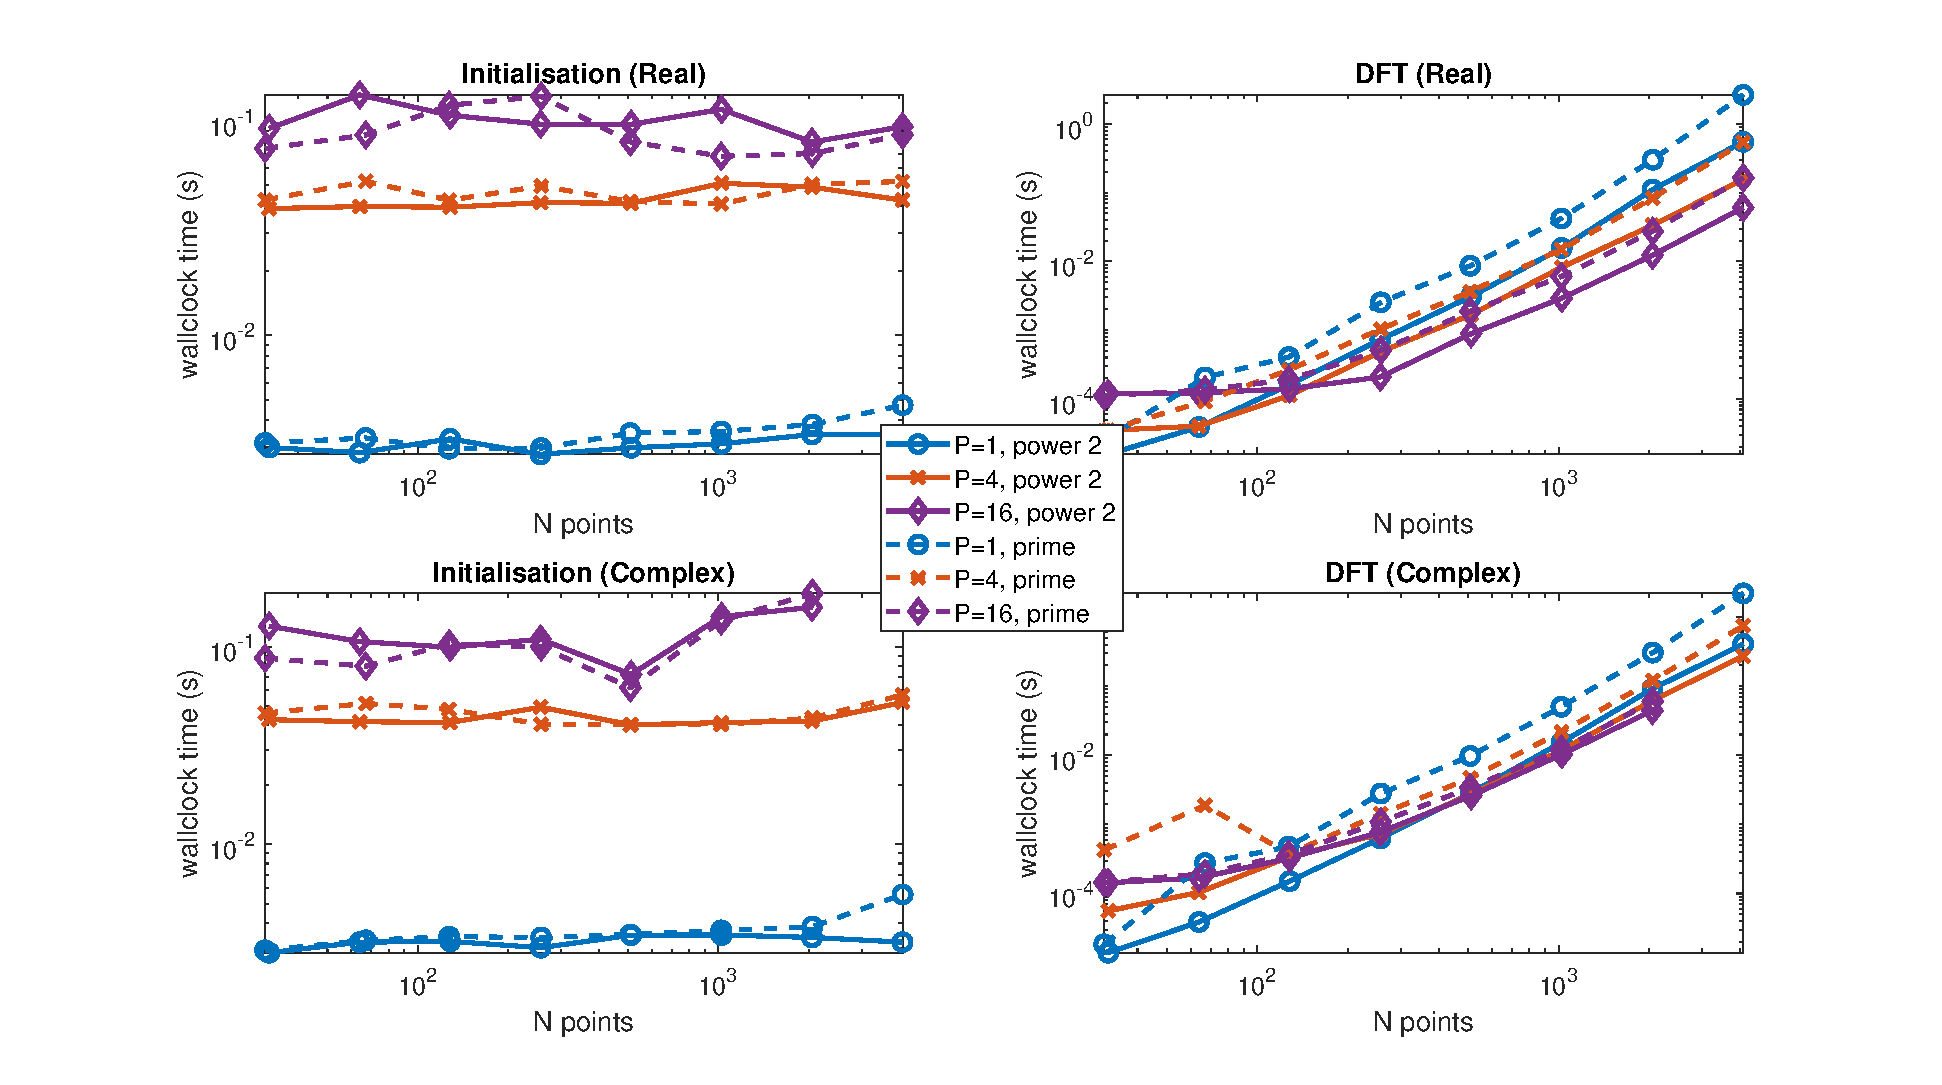
\includegraphics[width=\linewidth]{../results/mkl_2d_mpi.eps}
  \caption{Initialisation and DFT execution times of distributed MKL library applied to 2D signal as a function of the
    number of points, $N,$ and varying the number of MPI processes, $P,$ with one thread per process.}
  \label{2DDistMKL}
\end{figure}

\begin{figure}[htb]
    \centering
    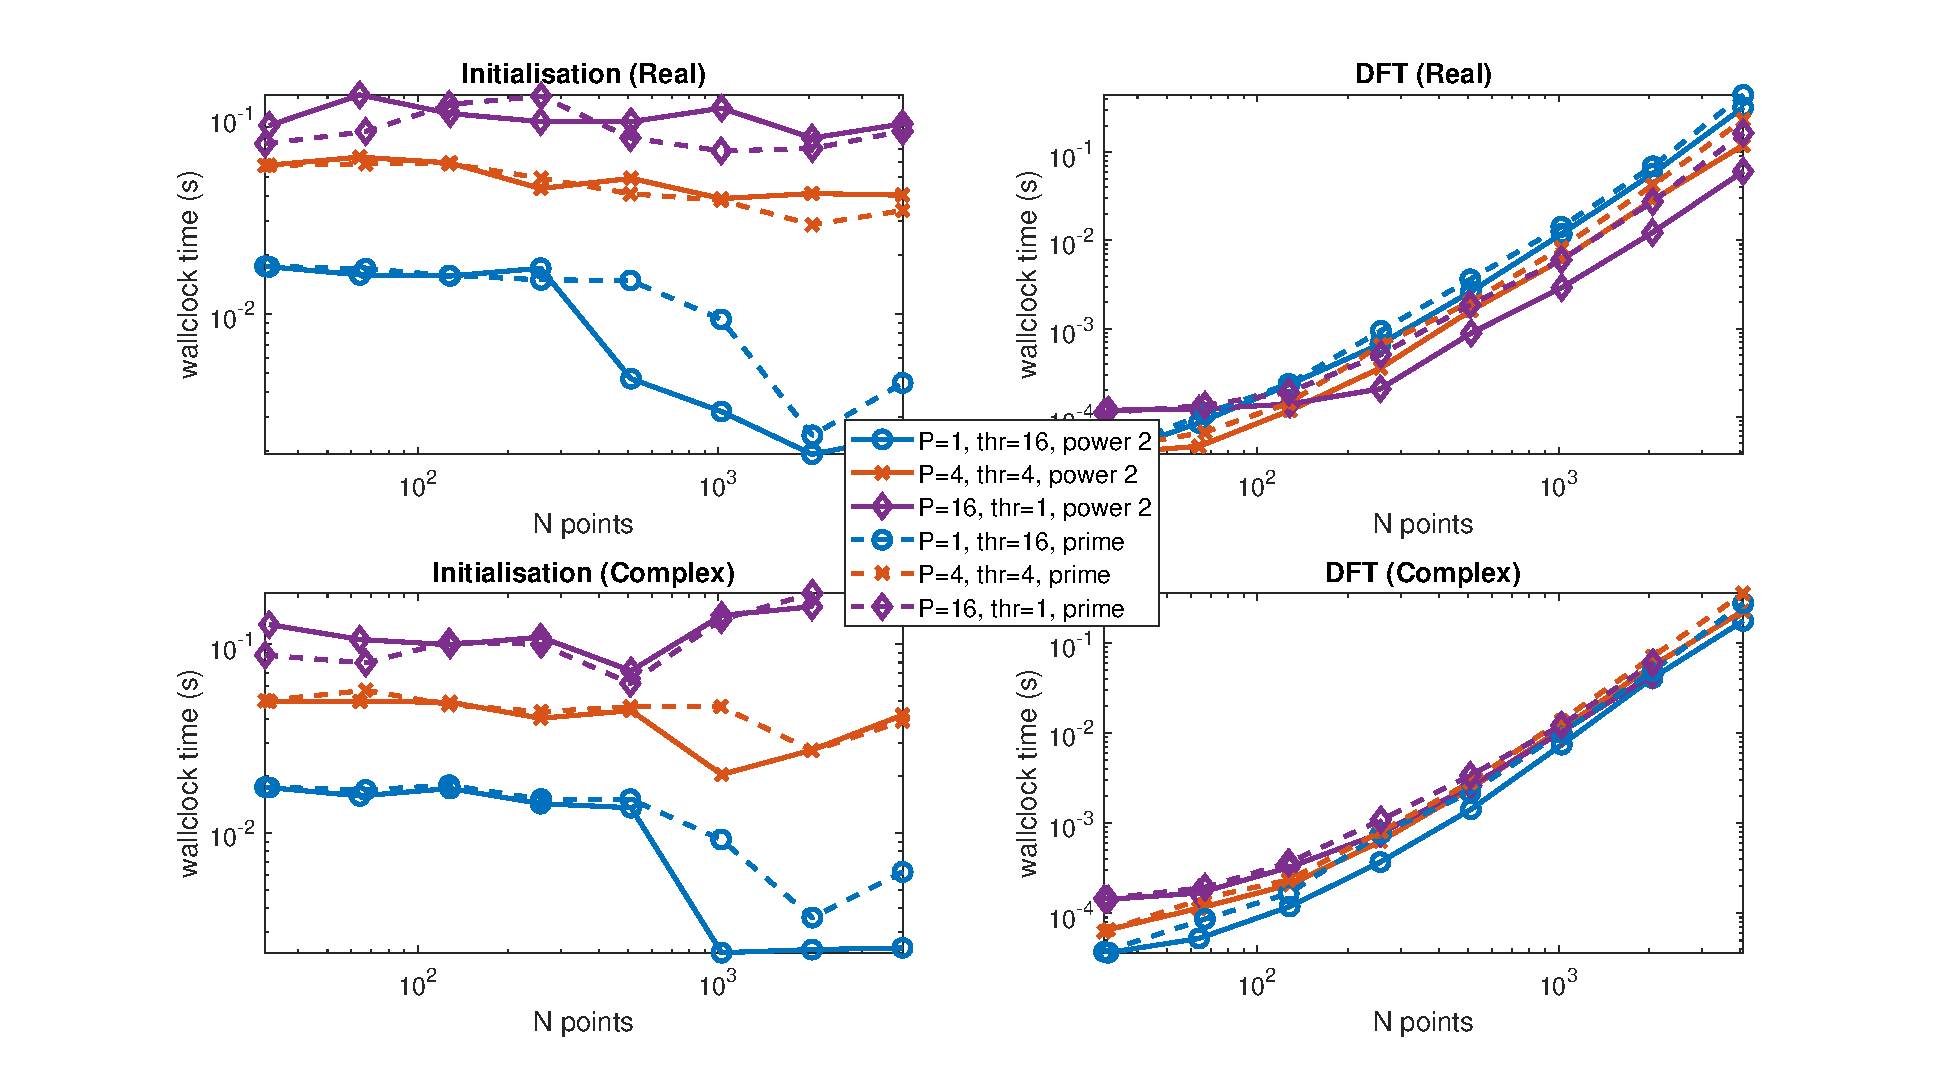
\includegraphics[width=\linewidth]{../results/mkl_2d_mpi_thr.eps}
  \caption{Initialisation and DFT execution times of distributed MKL library applied to 2D signal as a function of the
    number of points, $N,$ and varying the number of MPI processes, $P,$ and threads, $thr,$ whilst maintaining $P\times thr=16.$}
  \label{2DDistMKL16}
\end{figure}

\subsection{Comparison of distributed libraries for 2D benchmark}\label{Sec:2DDistComp}


\begin{figure}[htb]
    \centering
    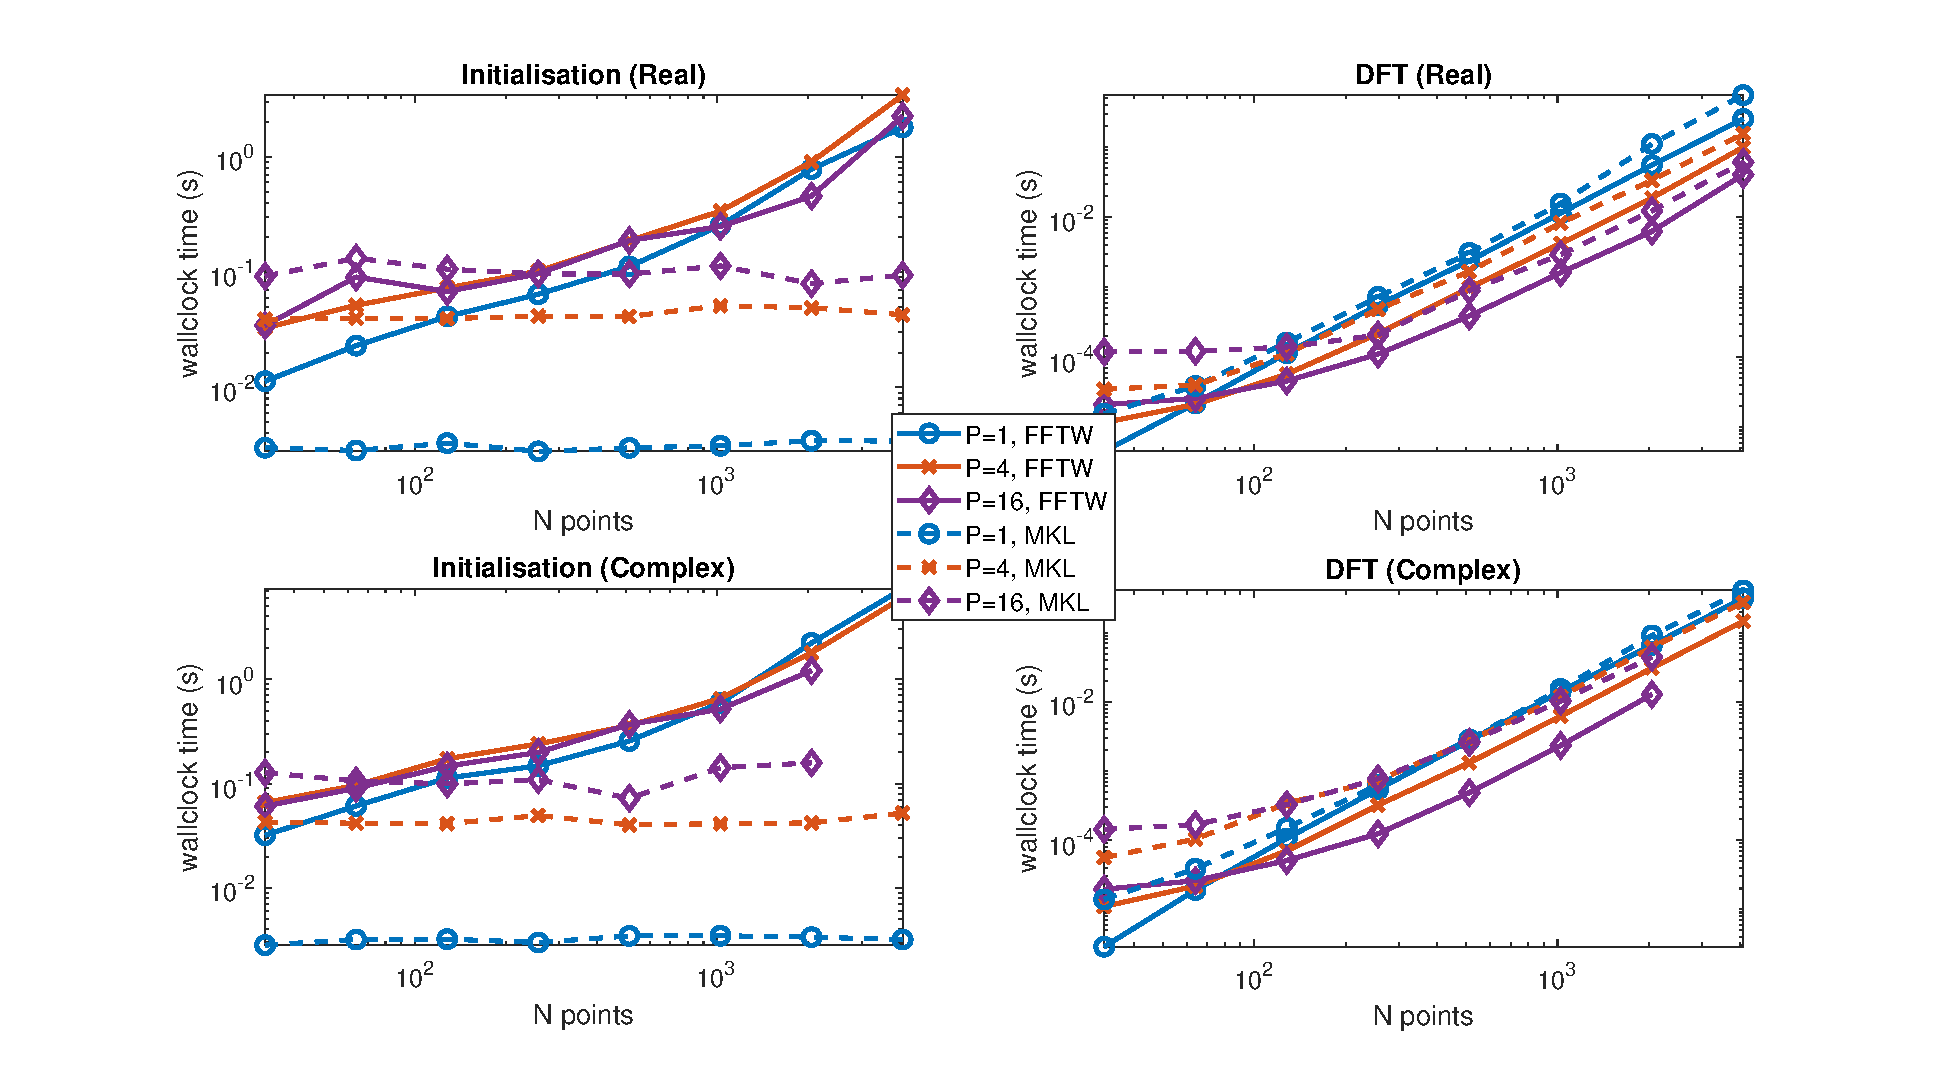
\includegraphics[width=\linewidth]{../results/fftw_mkl_2_2d_mpi.eps}
  \caption{Initialisation and DFT execution times of distributed FFTW and MKL libraries applied to 2D signal as a function of the
    number of points, $N,$ and varying the number of MPI processes, $P,$ with one thread per process. $N$ is a power of 2.}
  \label{2DDistFFTWMKL2}
\end{figure}


\begin{figure}[htb]
    \centering
    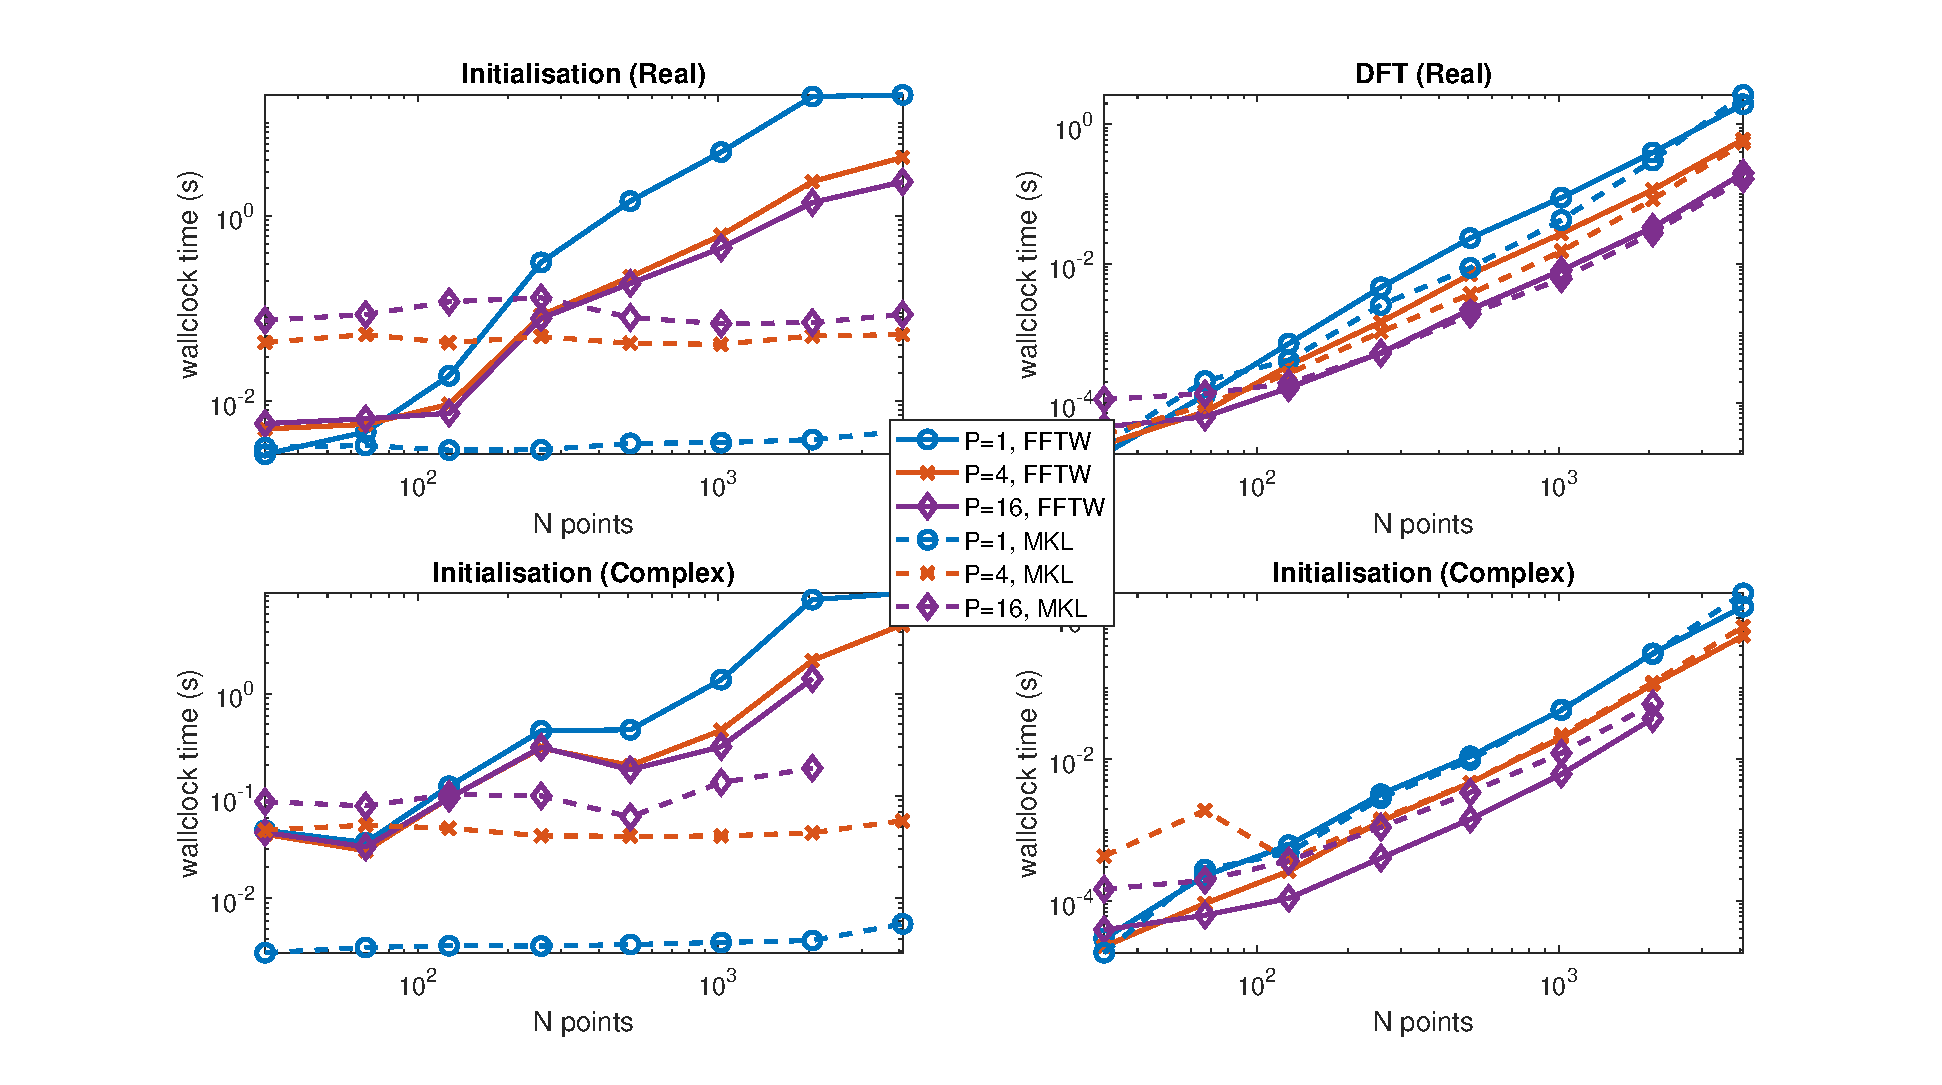
\includegraphics[width=\linewidth]{../results/fftw_mkl_prime_2d_mpi.eps}
  \caption{Initialisation and DFT execution times of distributed FFTW and MKL libraries applied to 2D signal as a function of the
    number of points, $N,$ and varying the number of MPI processes, $P,$ with one thread per process. $N$ is a prime number.}
  \label{2DDistFFTWMKLprime}
\end{figure}



\section{3D Distributed Benchmark Results}\label{Sec:3DDistr}

\subsection{3D Distributed FFTW Library}\label{Sec:3DDistFFTW}

\begin{figure}[htb]
    \centering
    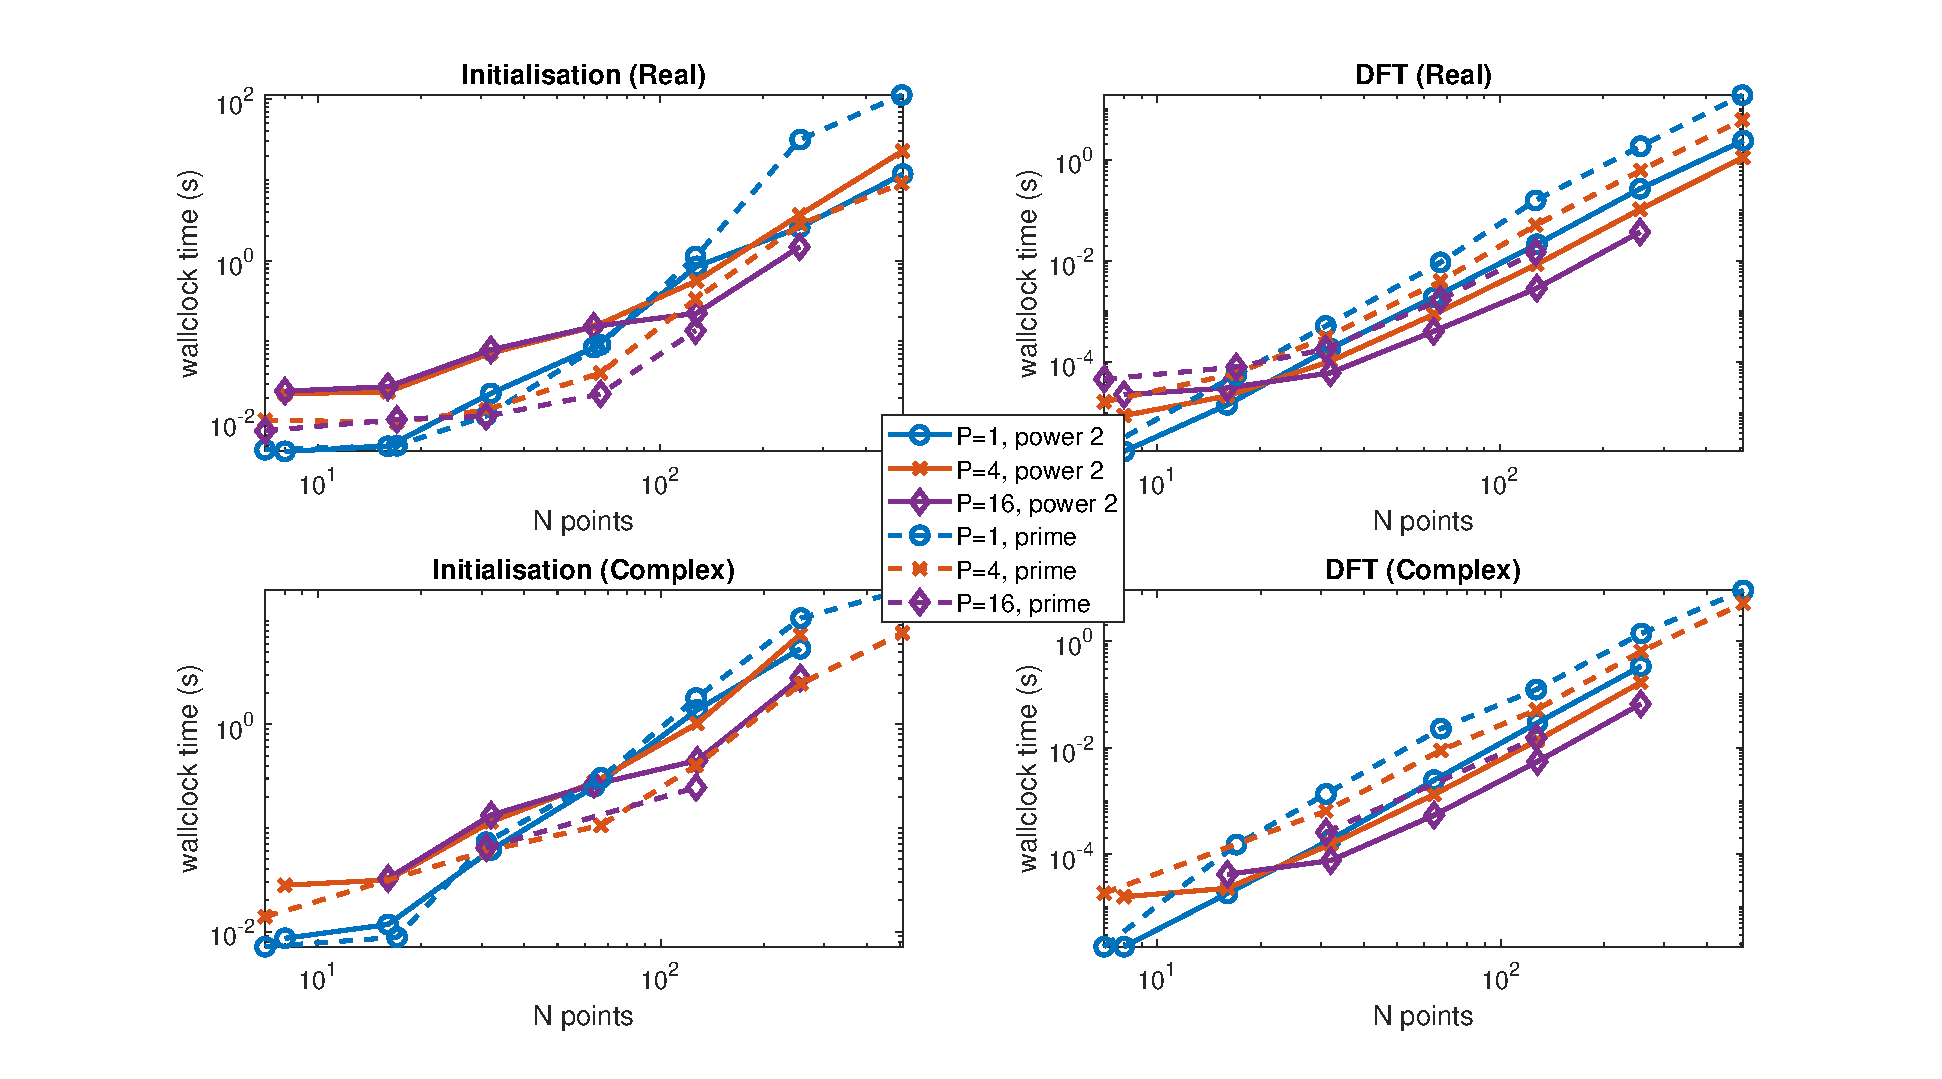
\includegraphics[width=\linewidth]{../results/fftw_3d_mpi.eps}
  \caption{Initialisation and DFT execution times of distributed FFTW library applied to 3D signal as a function of the
    number of points, $N,$ and varying the number of MPI processes, $P,$ with one thread per process.}
  \label{3DDistFFTW}
\end{figure}

\begin{figure}[htb]
    \centering
    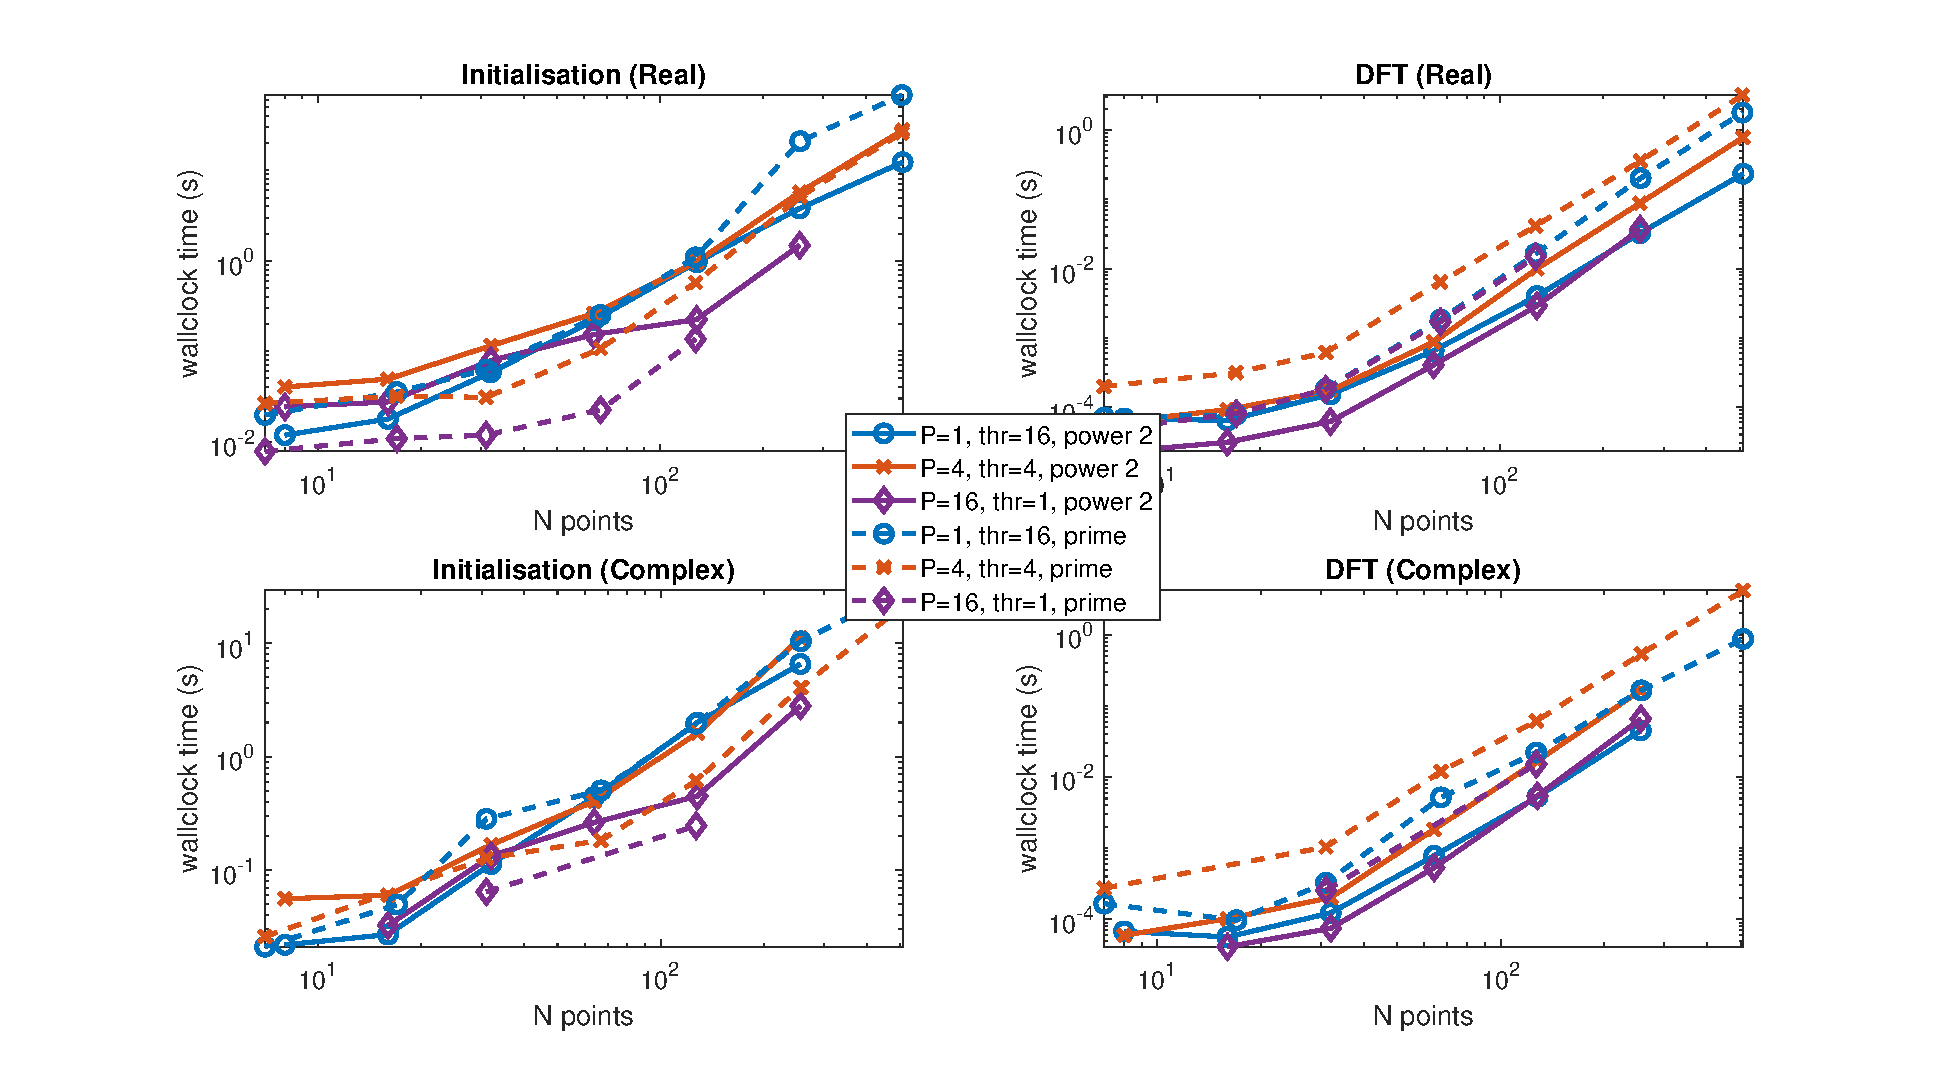
\includegraphics[width=\linewidth]{../results/fftw_3d_mpi_thr.eps}
  \caption{Initialisation and DFT execution times of distributed FFTW library applied to 3D signal as a function of the
    number of points, $N,$ and varying the number of MPI processes, $P,$ and threads, $thr,$ whilst maintaining $P\times thr=16.$}
  \label{3DDistFFTW16}
\end{figure}



\subsection{3D Distributed MKL Library}\label{Sec:3DDistMKL}

\begin{figure}[htb]
    \centering
    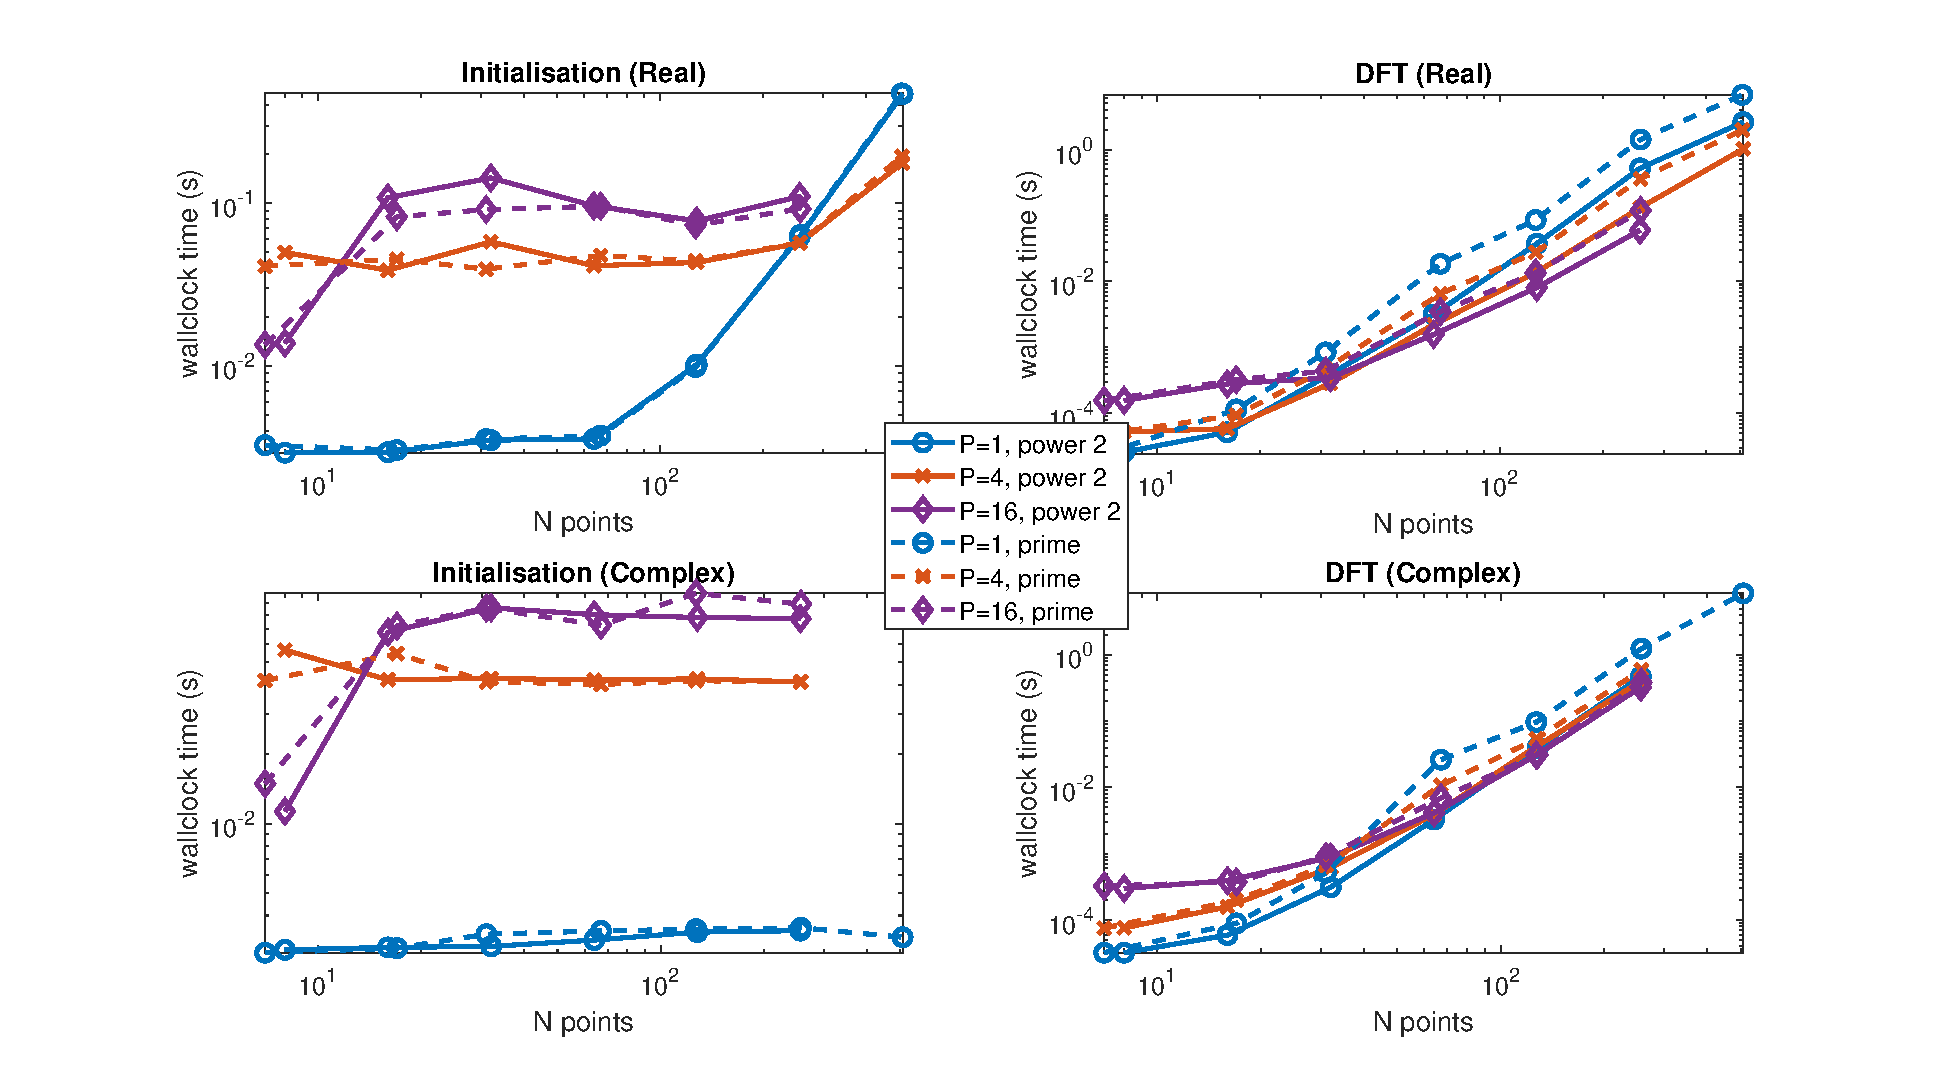
\includegraphics[width=\linewidth]{../results/mkl_3d_mpi.eps}
  \caption{Initialisation and DFT execution times of distributed MKL library applied to 3D signal as a function of the
    number of points, $N,$ and varying the number of MPI processes, $P,$ with one thread per process.}
  \label{3DDistMKL}
\end{figure}

\begin{figure}[htb]
    \centering
    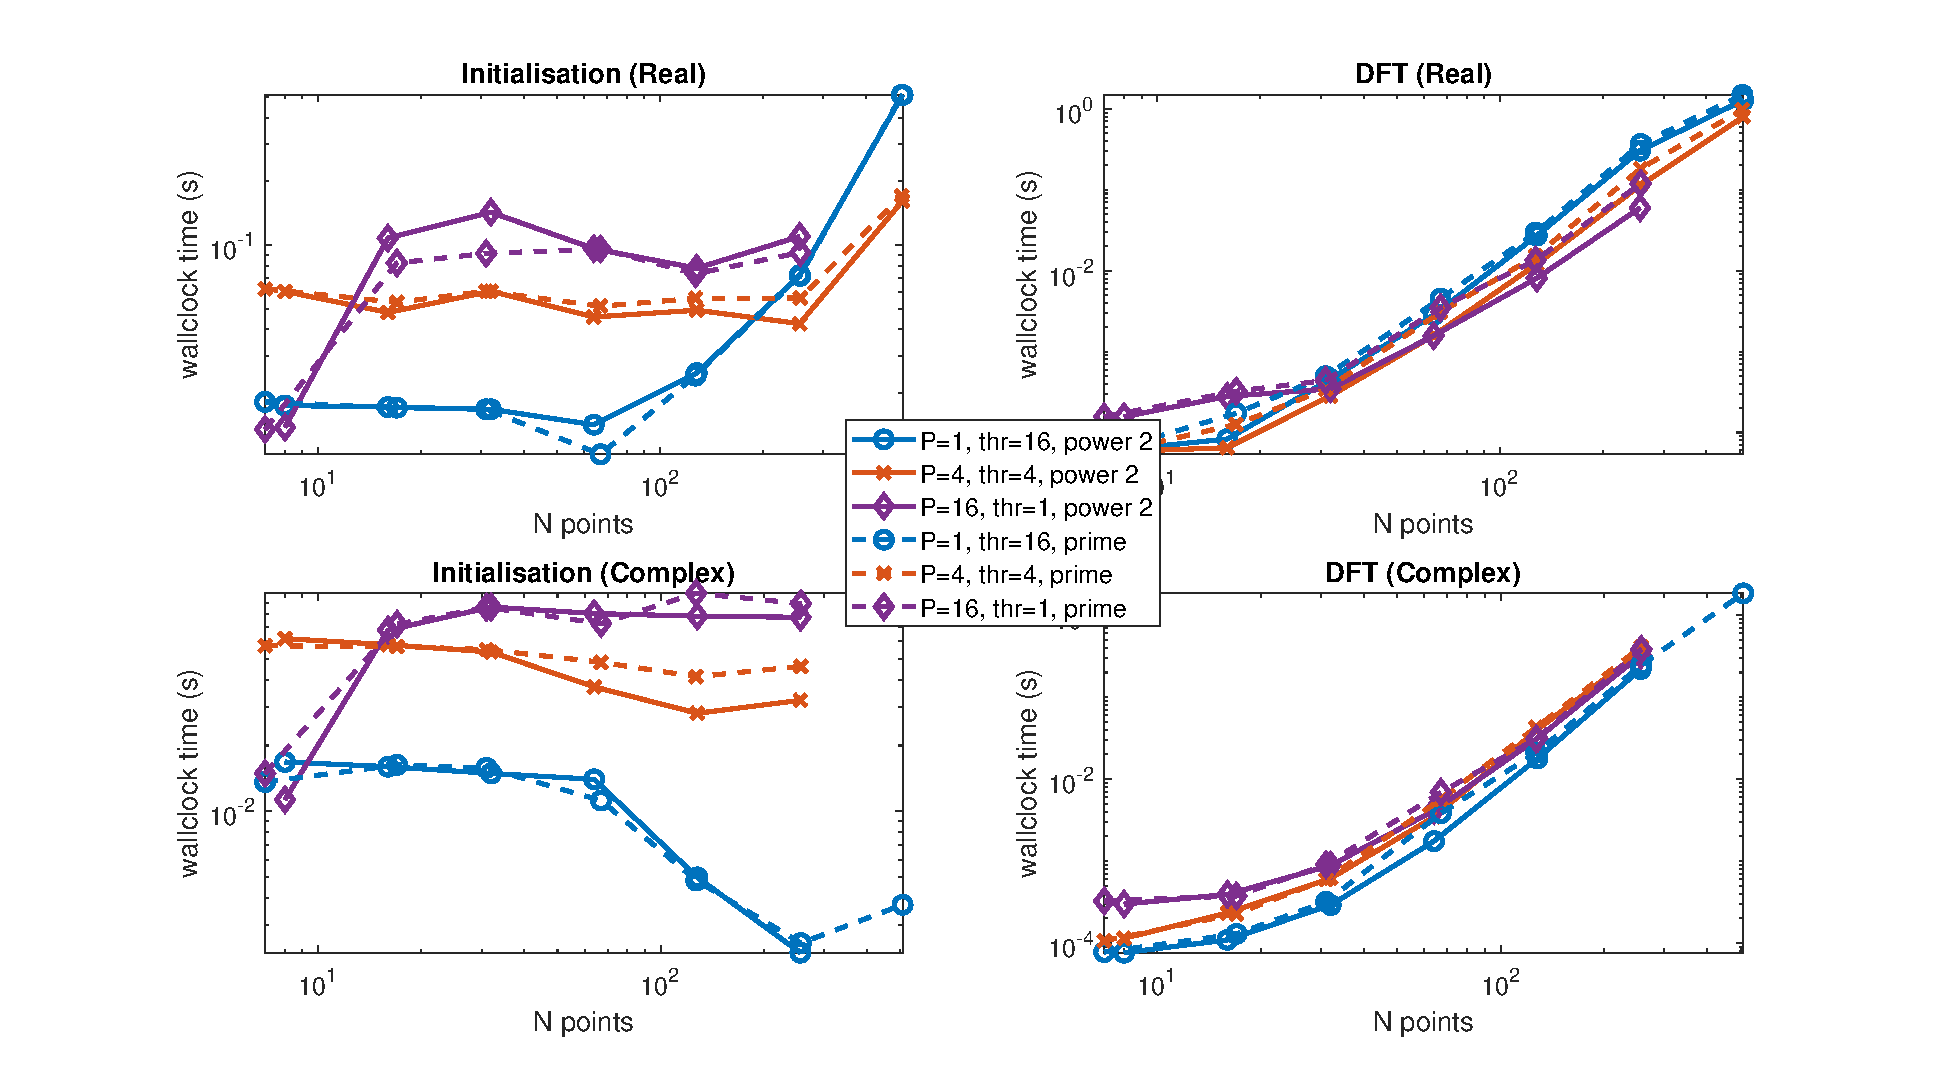
\includegraphics[width=\linewidth]{../results/mkl_3d_mpi_thr.eps}
  \caption{Initialisation and DFT execution times of distributed MKL library applied to 3D signal as a function of the
    number of points, $N,$ and varying the number of MPI processes, $P,$ and threads, $thr,$ whilst maintaining $P\times thr=16.$}
  \label{3DDistMKL16}
\end{figure}




\subsection{3D Distributed P3DFFT Library}\label{Sec:3DDistP3DFFT}

\begin{figure}[htb]
    \centering
    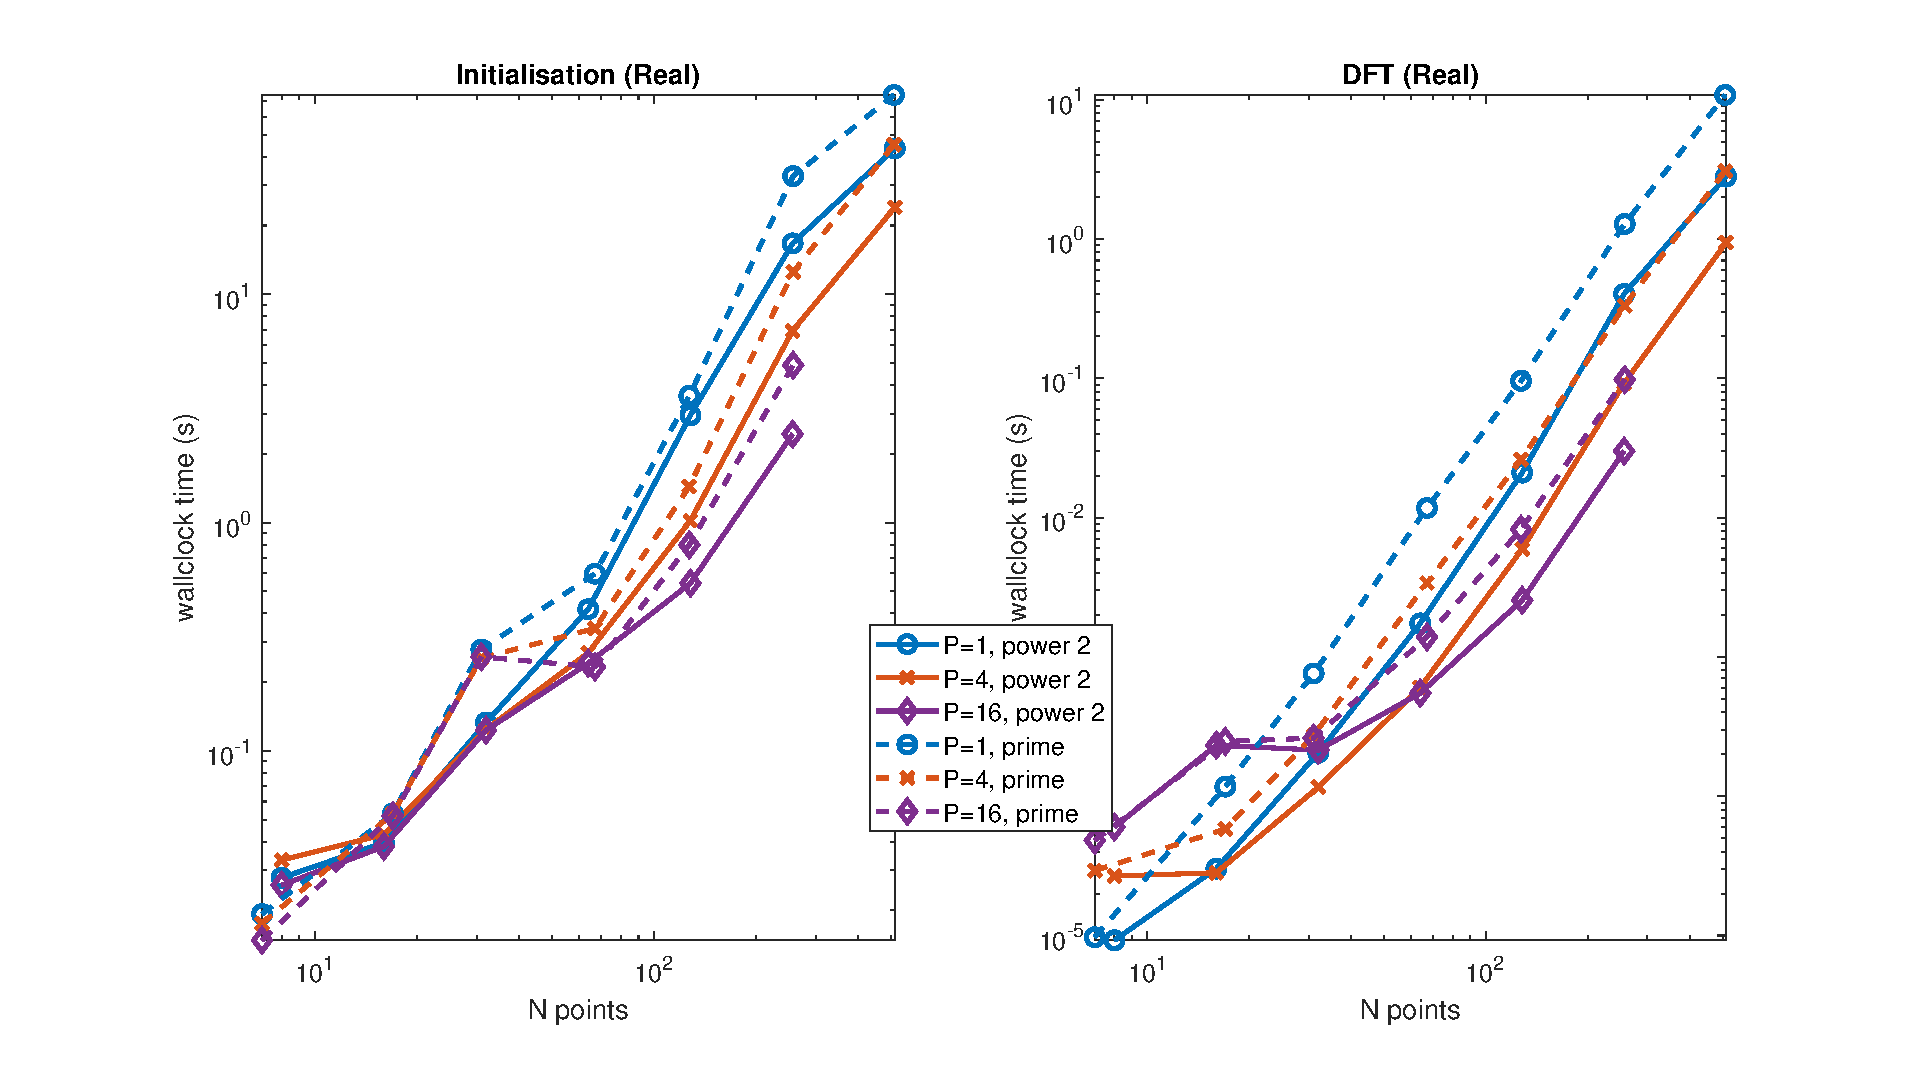
\includegraphics[width=\linewidth]{../results/p3dfft_3d_mpi.eps}
  \caption{Initialisation and DFT execution times of distributed P3DFFT library applied to 3D signal as a function of the
    number of points, $N,$ and varying the number of MPI processes, $P,$ with one thread per process.}
  \label{3DDistP3DFFT}
\end{figure}

\begin{figure}[htb]
    \centering
    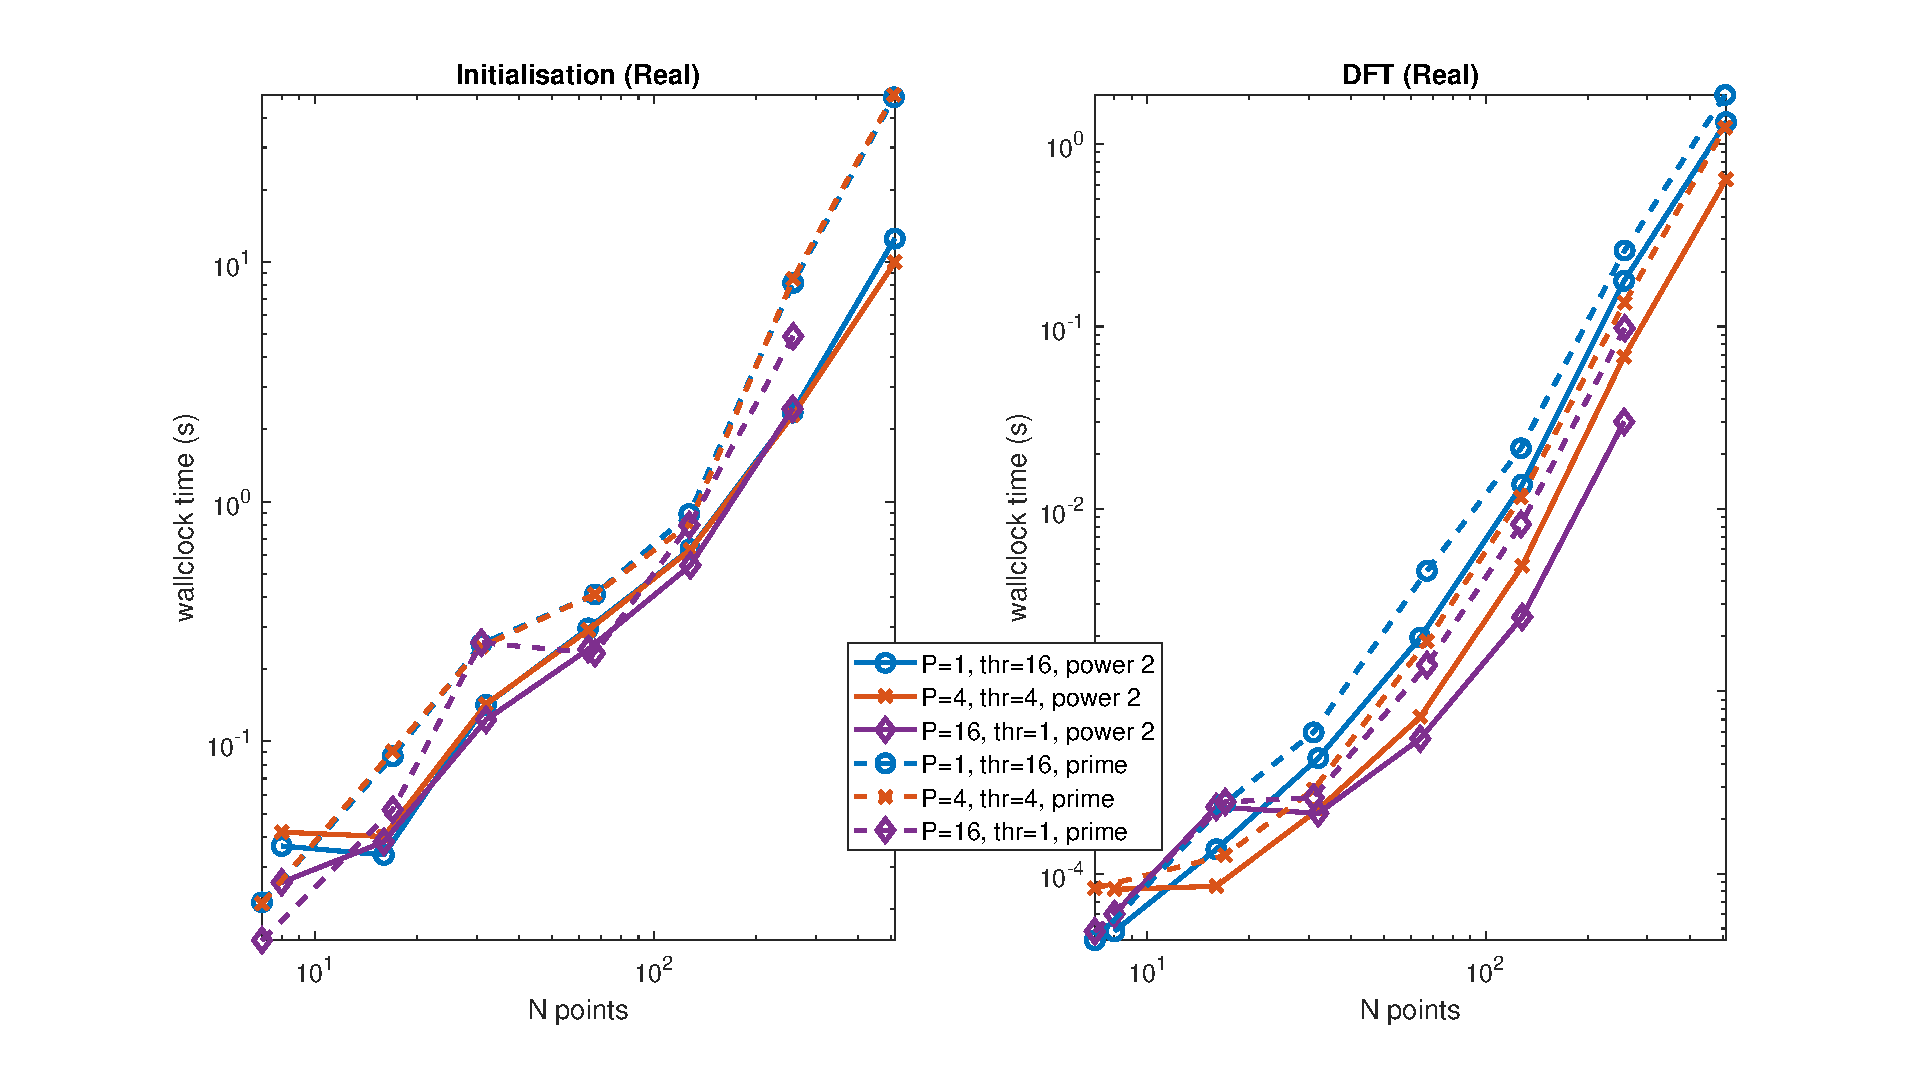
\includegraphics[width=\linewidth]{../results/p3dfft_3d_mpi_thr.eps}
  \caption{Initialisation and DFT execution times of distributed P3DFFT library applied to 3D signal as a function of the
    number of points, $N,$ and varying the number of MPI processes, $P,$ and threads, $thr,$ whilst maintaining $P\times thr=16.$}
  \label{3DDistP3DFFT16}
\end{figure}

\subsection{Comparison of distributed libraries for 3D benchmark}\label{Sec:3DDistComp}


\begin{figure}[htb]
    \centering
    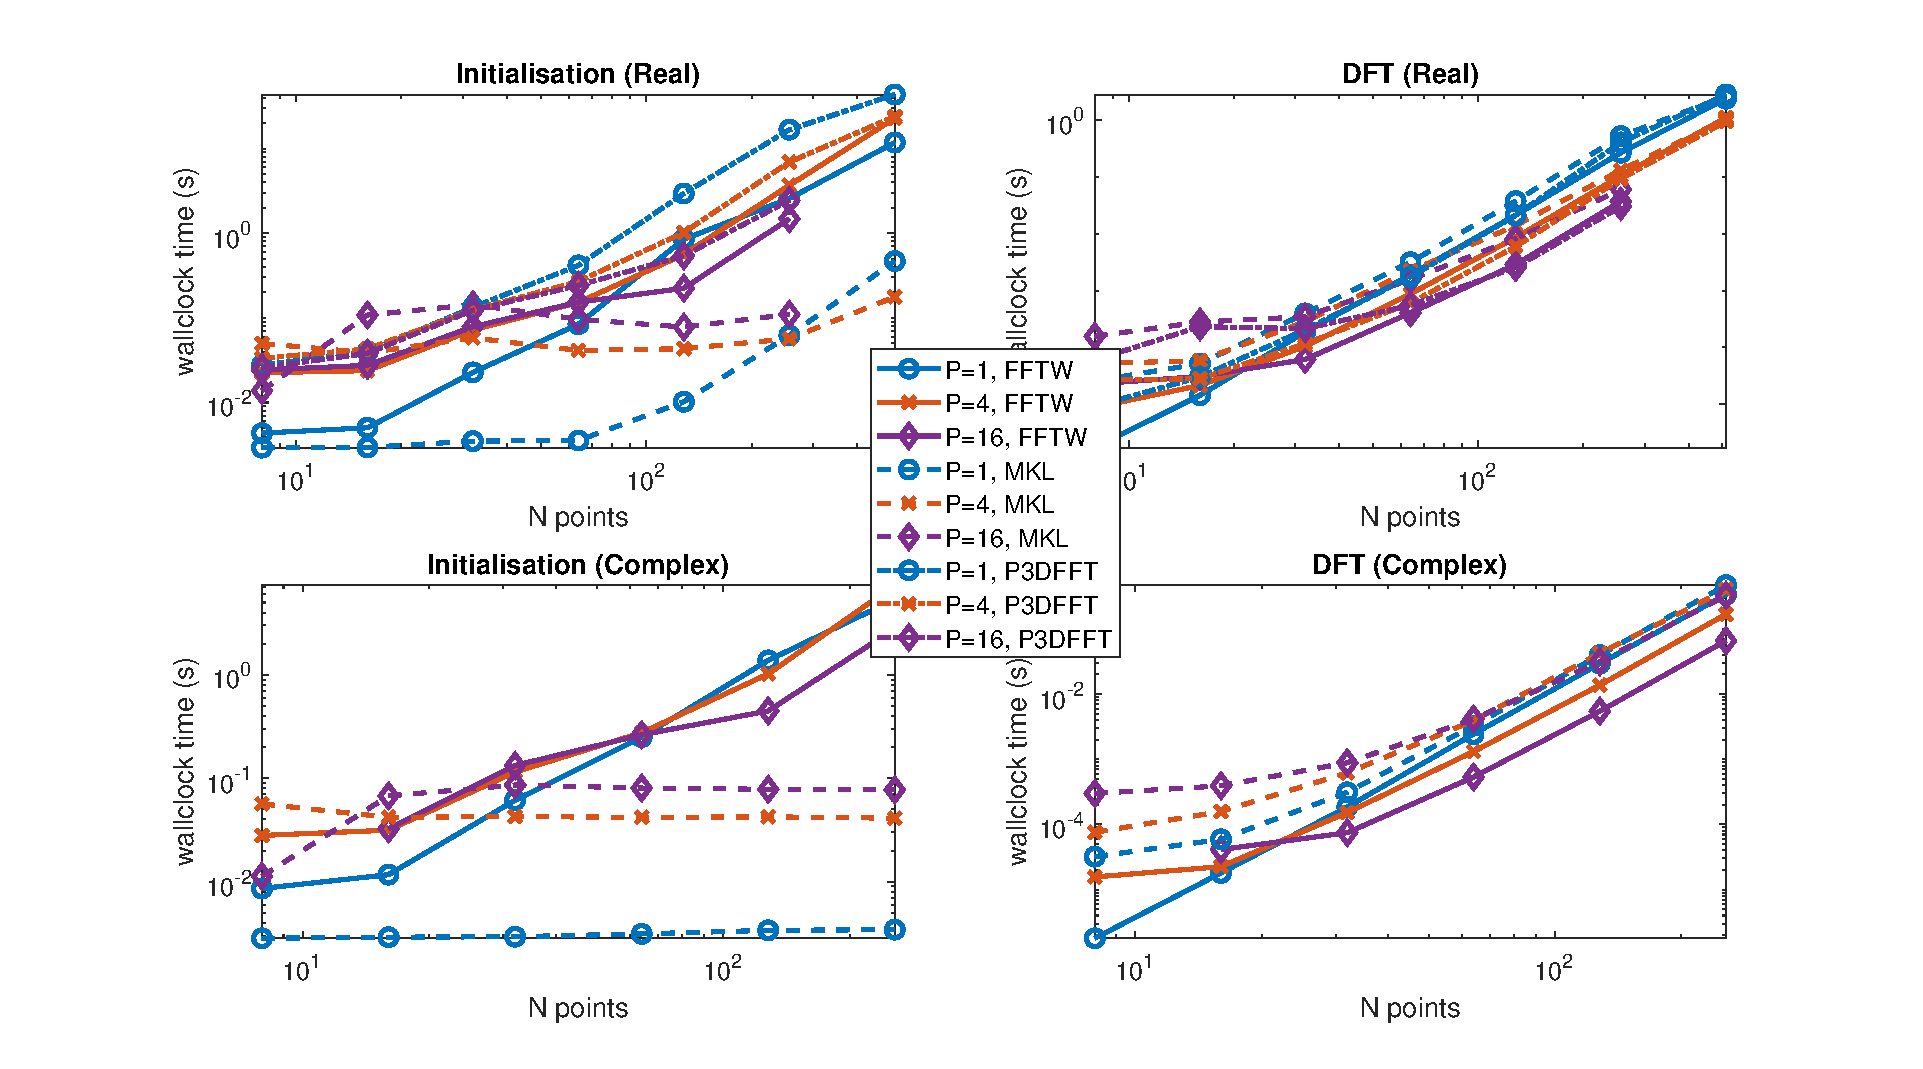
\includegraphics[width=\linewidth]{../results/fftw_mkl_p3dfft_2_3d_mpi.eps}
  \caption{Initialisation and DFT execution times of distributed FFTW, MKL and P3DFFT libraries applied to 3D signal as a function of the
    number of points, $N,$ and varying the number of MPI processes, $P,$ with one thread per process. $N$ is a power of 2.}
  \label{3DDistFFTWMKLP3DFFT2}
\end{figure}


\begin{figure}[htb]
    \centering
    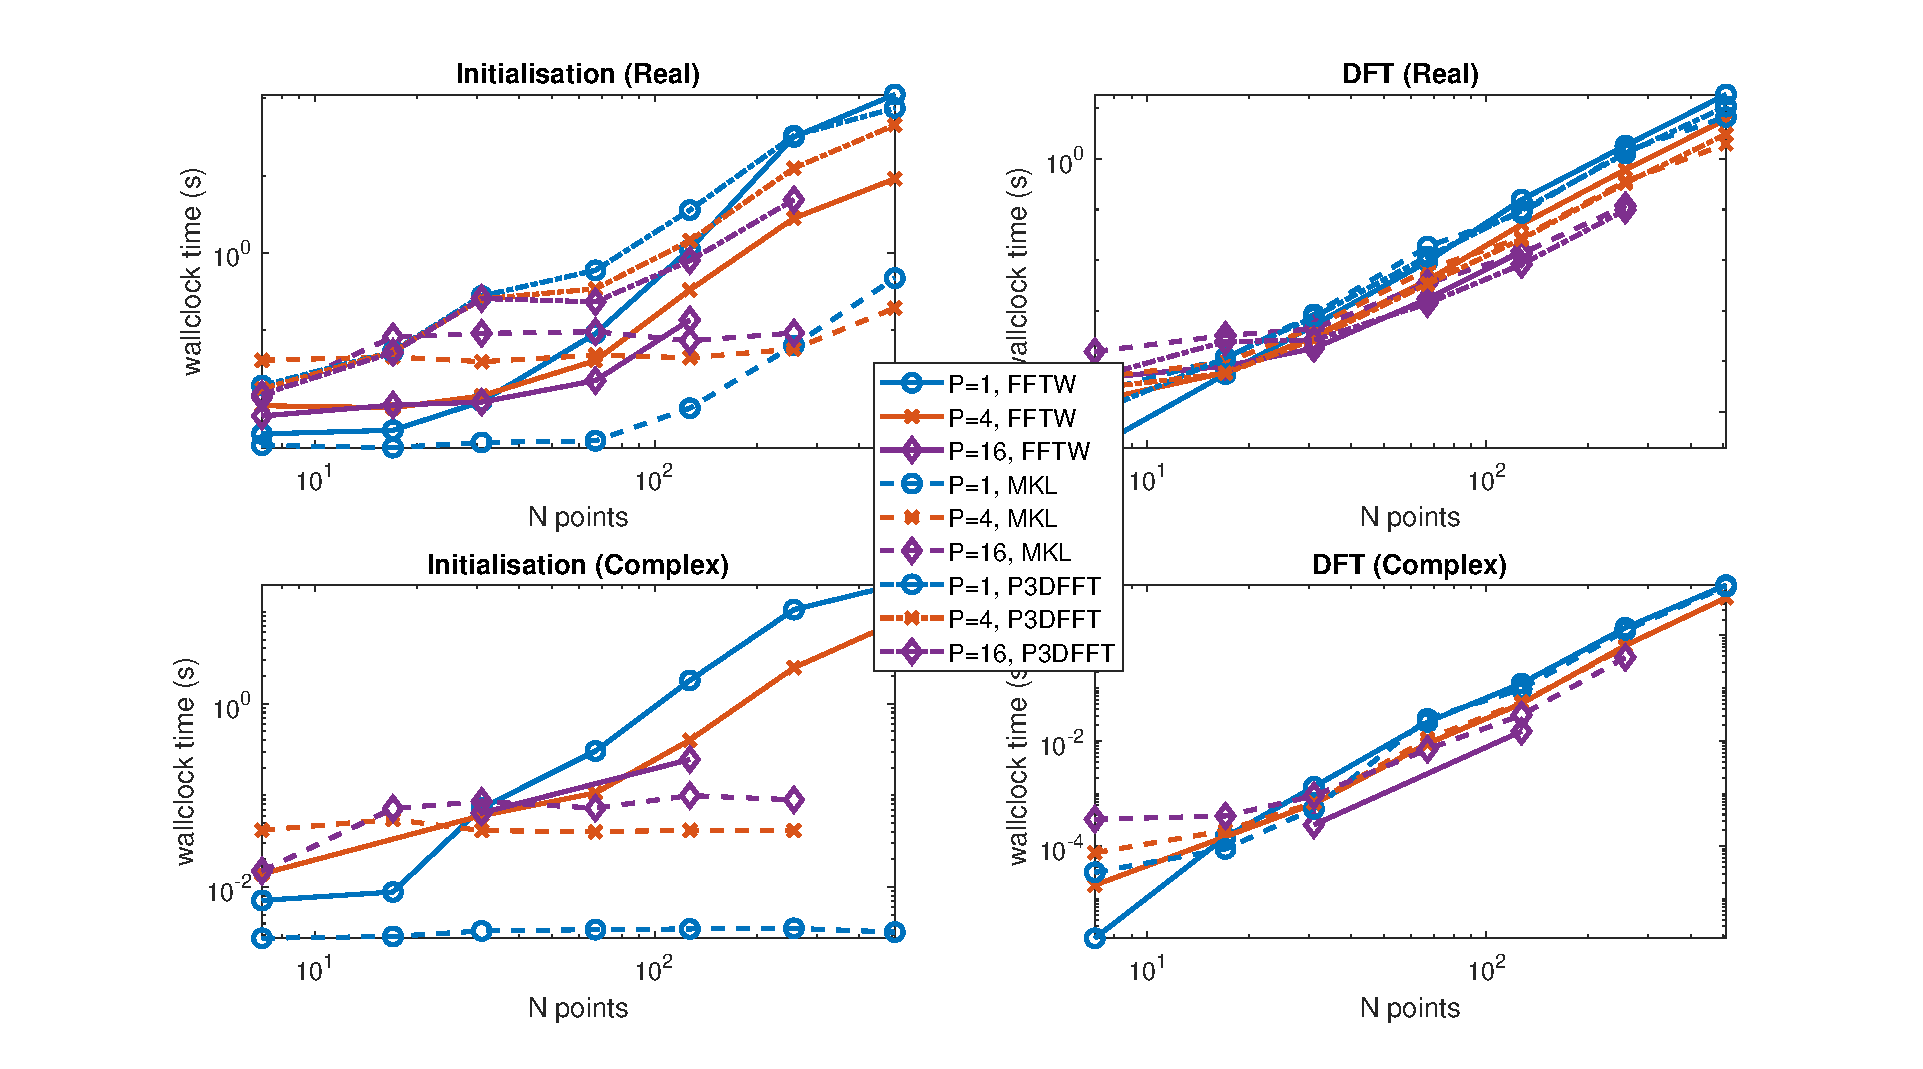
\includegraphics[width=\linewidth]{../results/fftw_mkl_p3dfft_prime_3d_mpi.eps}
  \caption{Initialisation and DFT execution times of distributed FFTW, MKL and P3DFFT libraries applied to 3D signal as a function of the
    number of points, $N,$ and varying the number of MPI processes, $P,$ with one thread per process. $N$ is a prime number.}
  \label{3DDistFFTWMKLP3DFFTprime}
\end{figure}



\section{Conclusions}\label{Sec:Conclusions}


\section*{Acknowledgements}
This work made use of computational support by CoSeC, the
Computational Science Centre for Research Communities, through its
Software Outlook activity.






\bibliographystyle{siam}
\bibliography{bib2017}






\end{document}
